\documentclass[a4paper,11pt,twoside]{book}
%\documentclass[11pt,twoside,letterpaper]{book}
\usepackage{a4wide}
\usepackage{multirow}
\usepackage{footnote}
\usepackage{amsbsy}
\usepackage{amsmath}
\usepackage{bm}
%\usepackage[dvips]{graphicx}
\usepackage{graphicx}
%\usepackage{fancyheadings}
\usepackage{fancyhdr}
%\setlength{\parindent}{0in}
%\setlength{\parskip}{0.05in}
\setlength{\parskip}{0.1in}

% Print only chapters in the Table Of Contents
\setcounter{tocdepth}{0} 

%\usepackage{a4wide}
\usepackage{color}
\def\red{\textcolor{red}}

%\parskip=2mm

% Ensure that blank pages don't have numbers or heading on them 
\makeatletter
\def\cleardoublepage{\clearpage\if@twoside \ifodd\c@page\else
 \hbox{}
 \vspace*{\fill}
 \thispagestyle{empty}
 \newpage\fi\fi}
\makeatother

% set fancy headings
\pagestyle{fancy}
\lhead[{\it \thepage}]{{\bf\it {\tt wannier90}: User Guide}}
\chead{}
\rhead[{\bf\it {\tt wannier90}: User Guide}]{{\it \thepage}}
\renewcommand{\headrulewidth}{0.2pt}
\lfoot{}
\cfoot{}
\rfoot{}
\renewcommand{\footrulewidth}{0pt}
\setlength{\footskip}{0.25in}
\setlength{\parindent}{0in}


%% This part slightly modifies the default definition of \chapter
%% (found in book.cls) to add a \hspace{2em} before numbered chapters.
\makeatletter
\def\@chapter[#1]#2{\ifnum \c@secnumdepth >\m@ne
                       \if@mainmatter
                         \refstepcounter{chapter}%
                         \typeout{\@chapapp\space\thechapter.}%
                         \addcontentsline{toc}{chapter}%
                                   {\hspace{2em}\protect\numberline{\thechapter}#1}%
                       \else
                         \addcontentsline{toc}{chapter}{#1}%
                       \fi
                    \else
                      \addcontentsline{toc}{chapter}{#1}%
                    \fi
                    \chaptermark{#1}%
                    \addtocontents{lof}{\protect\addvspace{10\p@}}%
                    \addtocontents{lot}{\protect\addvspace{10\p@}}%
                    \if@twocolumn
                      \@topnewpage[\@makechapterhead{#2}]%
                    \else
                      \@makechapterhead{#2}%
                      \@afterheading
                    \fi}
\makeatother

\title{{\tt wannier90}: User Guide}

\author{Version 1.2}

\date{15th January 2010}

% should be the last one to be loaded
\usepackage[plainpages=false,breaklinks=true,pdfborder=0 0 0,pdfdisplaydoctitle=true,bookmarksopen=true,bookmarksopenlevel=0,
            pdftitle={Wannier90 User Guide}]{hyperref}
\begin{document}
\newcommand{\wannier}{\texttt{wannier90}}
\newcommand{\postw}{\texttt{postw90}}
\newcommand{\bw}{\texttt{BoltzWann}}
\newcommand{\pwscf}{\textsc{pwscf}}
\newcommand{\QE}{\textsc{quantum-espresso}}
\newcommand{\Mkb}{\mathbf{M}^{(\mathbf{k},\mathbf{b})}}
\newcommand{\Ak}{\mathbf{A}^{(\mathbf{k})}}
\newcommand{\Uk}{\mathbf{U}^{(\mathbf{k})}}
\newcommand{\cond}{\item[$\star$]}
\newcommand{\omi}{\Omega_{\mathrm{I}}}
\newcommand{\omt}{\widetilde{\Omega}}
\newcommand{\bvec}[1]{\bm{\mathrm{#1}}}

\maketitle

\tableofcontents

%\listoftables

%\listoffigures

\part{Introduction}

\chapter{Introduction}

\section{Methodology}
Wannier90 computes Maximally Localised
Wannier Functions (MLWFs) following the method of Marzari and Vanderbilt (MV).\footnote{
{\it Maximally localized generalized Wannier functions for composite energy bands}
N. Marzari and D. Vanderbilt, Phys. Rev. B 56, 12847 (1997)}
For entangled energy bands  the method of
Souza, Marzari and Vanderbilt (SMV)\footnote{{\it Maximally localized
    Wannier functions for entangled energy bands} 
I. Souza, N. Marzari and D. Vanderbilt, Phys. Rev. B 65, 035109 (2002)}
is used.
We briefly introduce the methods and key definitions, but full details
can be found in the original papers. 

First principles codes typically solve the electronic structure of
periodic materials in terms of Bloch states, $\psi_{n{\bf k}}$. 
These extended states are characterised by a band index $n$ and crystal
momentum ${\bf k}$. An alternative representation can be given in terms
of spatially localised functions known as Wannier functions (WFs). The WF 
centred on a lattice site ${\bf R}$,  $w_{n{\bf R}}({\bf r})$, 
is written in terms of the set of Bloch states as
\begin{equation}
w_{n{\bf R}}({\bf r})=\frac{V}{(2\pi)^3}\int_{BZ} \left[\sum_{m} U^{({\bf
k})}_{mn} \psi_{m{\bf k}}({\bf r})\right]e^{-\mathrm{i}{\bf k}.{\bf R}} d{\bf k},
\end{equation}
where $\bf{U}^{({\bf k})}$ is a unitary matrix that mixes the Bloch
states at each 
${\bf k}$. $\bf{U}^{({\bf k})}$ is not uniquely defined and different choices
will lead to WFs with varying spatial localisations. We define the
spread $\Omega$
of the WFs as 
\begin{equation}
\Omega=\sum_n \left[\langle w_{n{\bf 0}}({\bf r})| r^2 | w_{n{\bf
      0}}({\bf r}) \rangle - | \langle w_{n{\bf 0}}({\bf r})| {\bf r} | w_{n{\bf
      0}}({\bf r}) \rangle |^2 \right].
\end{equation}
The total spread can be decomposed into a gauge invariant term
$\Omega_{\rm I}$ plus a term ${\tilde \Omega}$ that is dependant on the gauge
choice $\bf{U}^{({\bf k})}$. ${\tilde \Omega}$ can
be further divided into terms diagonal and off-diagonal in the WF basis,
$\Omega_{\rm D}$ and $\Omega_{\rm OD}$.
\begin{equation}
\Omega=\Omega_{\rm I}+{\tilde \Omega}=\Omega_{\rm I}+\Omega_{\rm D}+\Omega_{\rm OD}
\end{equation}
where
\begin{equation}
\Omega_{{\rm I}}=\sum_n \left[\langle w_{n{\bf 0}}({\bf r})| r^2 | w_{n{\bf
      0}}({\bf r}) \rangle - \sum_{{\bf R}m} \left| \langle w_{n{\bf R}}({\bf r})| {\bf r} | w_{n{\bf
      0}}({\bf r}) \rangle \right| ^2 \right]
\end{equation}
\begin{equation}
\Omega_{\rm D}=\sum_n \sum_{{\bf R}\neq{\bf 0}} |\langle w_{n{\bf R}}({\bf r})| {\bf r} |
w_{n{\bf 0}}({\bf r}) \rangle|^2 
\end{equation}
\begin{equation}
\Omega_{\rm OD}=\sum_{m\neq n} \sum_{{\bf R}} |\langle w_{m{\bf R}}({\bf
  r})| {\bf r} |
w_{n{\bf 0}}({\bf r}) \rangle |^2 
\end{equation}
The MV method minimises the gauge dependent spread $\tilde{\Omega}$ with respect the set
of $\bf{U}^{({\bf k})}$ to obtain MLWFs.

The Wannier90 code requires two ingredients from an initial electronic structure calculation.
\begin{enumerate}
\item The overlaps between the cell periodic part of the Bloch states $|u_{n{\bf k}}\rangle$ 
\begin{equation}
M_{mn}^{(\bf{k,b})}=\langle u_{m{\bf k}}|u_{n{\bf k}+{\bf b}}\rangle,
\end{equation}
where the vectors ${\bf b}$, which connect a given k-point with its neighbours, are determined
by the Wannier90 code according to the prescription outlined in MV.
\item As a starting guess the projection of the Bloch states
  $|\psi_{n\bf{k}}\rangle$ onto trial localised orbitals $|g_{n}\rangle$ 
\begin{equation}
A_{mn}^{(\bf{k})}=\langle \psi_{m{\bf k}}|g_{n}\rangle,
\end{equation}
\end{enumerate}
Note that $\bf{M}^{(\bf{k,b})}$, $\bf{A}^{(\bf{k})}$ and
$\bf{U}^{({\bf k})}$ are all 
small, $N_{{\rm wann}}\times N_{{\rm wann}}$ matrices, independent of
the basis set used to obtain the original Bloch states.  

To date the Wannier90 code has been
used in combination with electronic codes based on plane-waves and
pseudopotentials (norm-conserving and ``ultrasoft'') as well as mixed
basis set techniques such as FLAPW. 

\subsection{Entangled Energy Bands}
The above description is sufficient to obtain Wannier functions for an
isolated set of bands, such as the valence states in an insulator. In
order to obtain MLWFs for entangled energy bands we use the
``disentanglement'' procedure introduced in SMV.

We define an energy window (the ``outer window''). At a given
k-point $\bf{k}$, 
$N^{{\bf k}}_{{\rm win}}$ states lie within this energy window. We
obtain a set of 
$N_{{\rm wann}}$ Bloch states by performing a unitary
transformation amongst the Bloch states which fall within the energy window at each k-point:
 \begin{equation}
| u_{n{\bf k}}^{{\rm opt}}\rangle = \sum_{m\in N^{{\bf k}}_{{\rm win}}}
U^{{\rm dis}({\bf k})}_{mn} | u_{m{\bf k}}\rangle
\end{equation}
where $\bf{U}^{{\rm dis}({\bf k})}$ is a rectangular $N_{{\rm
 wann}}\times N^{{\bf k}}_{{\rm win}}$
 matrix\footnote{As
    $\bf{U}^{{\rm dis}({\bf k})}$ is a rectangular matrix this is a unitary
    operation in the sense that $(\bf{U}^{{\rm dis}({\bf k})})^{\dagger}\bf{U}^{{\rm dis}({\bf k})}=\bf{1}$.}. The set of $\bf{U}^{{\rm dis}({\bf k})}$ are obtained by minimising
 the gauge invariant spread $\Omega_{{\rm I}}$ within the outer energy
 window. The MV procedure can then be used to minimise $\tilde{\Omega}$
 and hence obtain MLWF for this optimal subspace.

It should be noted that the energy bands of this
optimal subspace may not correspond to any of the original energy
bands (due to mixing between states). In order to preserve exactly the
properties of a system in a given energy range (eg, around the Fermi
level) we introduce a second  energy window. States lying
within this inner, or ``frozen'', energy window are included unchanged
in the optimal subspace.

\subsection{Getting Help}
The latest version of the Wannier90 code and documentation can always be found at
{\tt 
\begin{quote}
http://www.wannier.org
\end{quote} }
There is a Wannier90 mailing list to
discuss issues in the development, the theory, and coding/algorithms
pertinent to maximally-localized Wannier functions.
You can register for this mailing list at
{\tt
\begin{quote}
http://www.democritos.it/mailman/listinfo/wannier
\end{quote} }

\subsection{Citation}
We ask that you acknowledge the use of Wannier90 in any publications
arising from the use of this code through the following reference
\begin{quote}
[ref] A. A. Mostofi, J. R. Yates,
N. Marzari, I. Souza and D. Vanderbilt,  

 http://www.wannier.org/                 
\end{quote}                                                              

It would also be appropriate to cite the original articles:\\\\
{\it Maximally localized generalized Wannier functions for composite energy bands}\\
N. Marzari and D. Vanderbilt, Phys. Rev. B 56, 12847 (1997)\\\\
{\it Maximally localized Wannier functions for entangled energy bands}\\
I. Souza, N. Marzari and D. Vanderbilt, Phys. Rev. B 65, 035109 (2002)


\subsection{Credits}
The present release of Wannier90 was written by Arash Mostofi (Marzari
group @ MIT) and Jonathan Yates (Souza Group @ UCB/LBNL). Wannier90 is
based on routines written in 1996-7 for occupied bands by Nicola Marzari
and David Vanderbilt and for entangled bands by Ivo Souza, Nicola Marzari,
and David Vanderbilt in 2000-1. 

Acknowledgements: Malgorzata Wierzbowska and Stefano de Gironcoli (pwscf interface);
Michel Posternak (LAPW interface and original plotting routines). 

Wannier90 \copyright 1997-2006 Jonathan Yates, Arash
Mostofi, Nicola Marzari, Ivo Souza, David Vanderbilt      

\subsection{Licence}
All the material in this distribution is free software; you can
redistribute it and/or 
modify it under the terms of the GNU General Public License
as published by the Free Software Foundation; either version 2
of the License, or (at your option) any later version.

This program is distributed in the hope that it will be useful,
but WITHOUT ANY WARRANTY; without even the implied warranty of
MERCHANTABILITY or FITNESS FOR A PARTICULAR PURPOSE.  See the
GNU General Public License for more details.

You should have received a copy of the GNU General Public License
along with this program; if not, write to the Free Software
Foundation, Inc., 51 Franklin Street, Fifth Floor, Boston, MA  02110-1301, USA.


 


\part{\texttt{wannier90.x}\label{part:w90}}

%!TEX root=./user_guide.tex
\chapter{Methodology}\label{sec:method}
\wannier\ computes maximally-localised Wannier functions (MLWF)
following the method of Marzari and Vanderbilt
(MV)~\cite{marzari-prb97}.  For entangled energy bands, the method of
Souza, Marzari and Vanderbilt (SMV)~\cite{souza-prb01} is used. We
introduce briefly the methods and key definitions here, but full
details can be found in the original papers and in
Ref.~\cite{mostofi-cpc08}.

First-principles codes typically solve the electronic structure of
periodic materials in terms of Bloch states, $\psi_{n{\bf k}}$. 
These extended states are characterised by a band index $n$ and crystal
momentum ${\bf k}$. An alternative representation can be given in terms
of spatially localised functions known as Wannier functions (WF). The WF 
centred on a lattice site ${\bf R}$, $w_{n{\bf R}}({\bf r})$, 
is written in terms of the set of Bloch states as
\begin{equation}
w_{n{\bf R}}({\bf r})=\frac{V}{(2\pi)^3}\int_{\mathrm{BZ}}
\left[\sum_{m} U^{({\bf k})}_{mn} \psi_{m{\bf k}}({\bf
    r})\right]e^{-\mathrm{i}{\bf k}.{\bf R}} \:\mathrm{d}{\bf k} \ , 
\end{equation}
where $V$ is the unit cell volume, the integral is over the Brillouin
zone (BZ), and $\Uk$ is a unitary matrix that mixes the Bloch 
states at each ${\bf k}$. $\Uk$ is not uniquely defined and different
choices will lead to WF with varying spatial localisations. We define
the spread $\Omega$ of the WF as 
\begin{equation}
\Omega=\sum_n \left[\langle w_{n{\bf 0}}({\bf r})| r^2 | w_{n{\bf
      0}}({\bf r}) \rangle - | \langle w_{n{\bf 0}}({\bf r})| {\bf r}
      | w_{n{\bf 0}}({\bf r}) \rangle |^2 \right].
\end{equation}
The total spread can be decomposed into a gauge invariant term
$\Omega_{\rm I}$ plus a term ${\tilde \Omega}$ that is dependant on the gauge
choice $\Uk$. ${\tilde \Omega}$ can
be further divided into terms diagonal and off-diagonal in the WF basis,
$\Omega_{\rm D}$ and $\Omega_{\rm OD}$,
\begin{equation}
\Omega=\Omega_{\rm I}+{\tilde \Omega}=\Omega_{\rm I}+\Omega_{\rm
  D}+\Omega_{\rm OD} 
\end{equation}
where
\begin{equation}
\Omega_{{\rm I}}=\sum_n \left[\langle w_{n{\bf 0}}({\bf r})| r^2 | w_{n{\bf
      0}}({\bf r}) \rangle - \sum_{{\bf R}m} \left| \langle w_{n{\bf
      R}}({\bf r})| {\bf r} | w_{n{\bf 0}}({\bf r}) \rangle \right| ^2
      \right] 
\end{equation}
\begin{equation}
\Omega_{\rm D}=\sum_n \sum_{{\bf R}\neq{\bf 0}} |\langle w_{n{\bf
    R}}({\bf r})| {\bf r} | w_{n{\bf 0}}({\bf r}) \rangle|^2 
\end{equation}
\begin{equation}
\Omega_{\rm OD}=\sum_{m\neq n} \sum_{{\bf R}} |\langle w_{m{\bf R}}({\bf
  r})| {\bf r} | w_{n{\bf 0}}({\bf r}) \rangle |^2 
\end{equation}
The MV method minimises the gauge dependent spread $\tilde{\Omega}$
with respect the set of $\Uk$ to obtain MLWF.

\wannier\ requires two ingredients from an initial electronic
structure calculation. 
\begin{enumerate}
\item The overlaps between the cell periodic part of the Bloch states
  $|u_{n{\bf k}}\rangle$  
\begin{equation}
M_{mn}^{(\bf{k,b})}=\langle u_{m{\bf k}}|u_{n{\bf k}+{\bf b}}\rangle,
\end{equation}
where the vectors ${\bf b}$, which connect a given k-point with its
neighbours, are determined by \wannier\ according to the prescription
outlined in Ref.~\cite{marzari-prb97}.
\item As a starting guess the projection of the Bloch states
  $|\psi_{n\bf{k}}\rangle$ onto trial localised orbitals $|g_{n}\rangle$ 
\begin{equation}
A_{mn}^{(\bf{k})}=\langle \psi_{m{\bf k}}|g_{n}\rangle,
\end{equation}
\end{enumerate}
Note that $\Mkb$, $\Ak$ and $\Uk$ are all small, $N \times N$
matrices\footnote{Technically, this is true for the case of an
  isolated group of $N$ bands from which we obtain $N$ MLWF. When
  using the disentanglement procedure of Ref.~\cite{souza-prb01},
  $\Ak$, for example, is a rectangular matrix. See
  Section~\ref{sec:disentangle}.}  that are independent of the basis
set used to obtain the original Bloch states.

To date, \wannier\ has been used in combination with electronic codes
based on plane-waves and pseudopotentials (norm-conserving and
ultrasoft~\cite{vanderbilt-prb90}) as well as mixed basis set techniques such as
FLAPW~\cite{posternak-prb02}.

\section{Entangled Energy Bands}\label{sec:disentangle}
The above description is sufficient to obtain MLWF for an isolated set
of bands, such as the valence states in an insulator. In order to
obtain MLWF for entangled energy bands we use the ``disentanglement''
procedure introduced in Ref.~\cite{souza-prb01}.

We define an energy window (the ``outer window''). At a given
k-point $\bf{k}$, $N^{({\bf k})}_{{\rm win}}$ states lie within this
energy window. We obtain a set of $N$ Bloch states by
performing a unitary transformation amongst the Bloch states which
fall within the energy window at each k-point: 
 \begin{equation}
| u_{n{\bf k}}^{{\rm opt}}\rangle = \sum_{m\in N^{({\bf k})}_{{\rm win}}}
U^{{\rm dis}({\bf k})}_{mn} | u_{m{\bf k}}\rangle
\end{equation}
where $\bf{U}^{{\rm dis}({\bf k})}$ is a rectangular $N^{({\bf k})}_{{\rm win}} \times N$
 matrix\footnote{As ${\bf U}^{{\rm dis}({\bf k})}$ is a rectangular
 matrix this is a unitary operation in the sense that $({\bf U}^{{\rm
 dis}({\bf k})})^{\dagger}{\bf U}^{{\rm dis}({\bf k})}={\bf 1}_N$.}. The
 set of $\bf{U}^{{\rm dis}({\bf k})}$ are obtained by minimising 
 the gauge invariant spread $\Omega_{{\rm I}}$ within the outer energy
 window. The MV procedure can then be used to minimise $\tilde{\Omega}$
 and hence obtain MLWF for this optimal subspace.

It should be noted that the energy bands of this optimal subspace may
not correspond to any of the original energy bands (due to mixing
between states). In order to preserve exactly the properties of a
system in a given energy range (e.g., around the Fermi level) we
introduce a second  energy window. States lying within this inner, or
``frozen'', energy window are included unchanged in the optimal
subspace.


\chapter{Parameters}

\section{Usage}
{\tt
\begin{quote}
wannier90.x [-pp] [seedname]
\end{quote} }
\begin{itemize}
\item{ {\tt seedname} If a seedname string is given the code will read its input
from a file {\tt seedname.win}. The default value is {\tt wannier}.}
\item { {\tt -pp} This optional flag tells the code to generate
a list of the required overlaps and then exit. 
This information is written to the file {\tt seedname.nnkp}.}
\end{itemize}

\section{win File}
The Wannier90 input file {\tt seedname.win} has a flexible free-form structure.

The ordering of the keywords is not significant. Case is ignored (so
\verb#num_bands# is the same as \verb#Num_Bands#). Characters after !, or \#
are treated as comments. Most keywords have a default value which is
used unless the keyword is 
given in the win file. Keywords can be set in any of the following ways
{\tt
\begin{quote}
num\_wann   4

num\_wann = 4

num\_wann : 4
\end{quote} }
A logical keyword can be set to {\tt .true.} using any of the following
strings: {\tt T}, {\tt true}, {\tt .true.}.

 For futher examples see Chapter \ref{chap:input} and the
 the Wannier90 Tutorial.


\section{Keyword List}
\label{parameter_data}

\begin{table}
\begin{center}
\begin{tabular}{|c|c|p{6cm}|}
\hline
Keyword & Type & Description \\
        &      &             \\
\hline\hline
\multicolumn{3}{|c|}{System Parameters} \\
\hline
{\sc num\_wann }   & I & Number of Wannier Functions \\
{\sc num\_bands }   & I & Number of bands passed to the code \\
{\sc unit\_cell\_cart }   & P & Unit cell vectors \\
{\sc atoms\_cart }*   & P & Positions of atoms in Cartesian coordinates \\
{\sc atoms\_frac }*   & R & Positions of atoms in lattice vectors \\
{\sc mp\_grid }   & I & Dimensions of the Monkhorst-Pack grid \\
%{\sc mp\_grid\_automatic }**   & L & Determine the kpoint automatically \\
{\sc kpoints }   & R & List of kpoints in the Monkhorst-Pack grid \\
{\sc num\_shells }   & I & Number of shells in finite difference formula \\
{\sc shell\_list }   & I & Which shells to use in finite difference formula \\
\hline
\end{tabular}
\caption[Parameter file keywords controlling system parameters.]
{win file keywords defining the system.  Argument types
are represented by, I for a integer, R for a real number, P for a
physical value, L for a logical value and S for a text string.\\
 {\footnotesize
* {\sc atoms\_cart } and  {\sc atoms\_frac } may not both be defined in
the same input file. }} 
\label{parameter_keywords1}
\end{center}
\end{table}


\begin{table}
\begin{center}
\begin{tabular}{|c|c|p{6cm}|}
\hline
Keyword & Type & Description \\
        &      &             \\
\hline\hline
\multicolumn{3}{|c|}{Job Control} \\
\hline
{\sc postproc\_setup }   & L & To output the nnkp file \\
{\sc cp\_pp }   & L & CP code post-processing \\
{\sc calc\_only\_a }   & L & Only recalculate the projections \\
{\sc exclude\_bands }   & I & List of bands to exclude from the calculation \\
{\sc restart }   & C & Restart from checkpoint file \\
{\sc iprint }   & I & Output verbosity level \\
{\sc length\_unit }   & S & System of units to output lengths \\
{\sc wvfn\_formated }   & L & Read the wavefunctions from a  (un)formatted file  \\
{\sc spin }   & S & Which spin channel to read \\
{\sc devel\_flag }   & S & Flag for development use \\
\hline
\end{tabular}
\caption[win file keywords.]
{win file keywords defining the system.  Argument types
are represented by, I for a integer, R for a real number, P for a
physical value, L for a logical value and S for a text string.\\
}
\label{parameter_keywords2}
\end{center}
\end{table}





\begin{table}
\begin{center}
\begin{tabular}{|c|c|p{6cm}|}
\hline
Keyword & Type & Description \\
        &      &             \\
\hline\hline
\multicolumn{3}{|c|}{Disentanglement Parameters} \\
\hline
{\sc dis\_win\_min }   & P & Bottom of the outer energy window \\
{\sc dis\_win\_max }   & P & Top of the outer energy window \\
{\sc dis\_froz\_min }   & P & Bottom of the inner (frozen) energy window \\
{\sc dis\_froz\_max }   & P & Top of the inner (frozen) energy window \\
{\sc dis\_num\_iter }   & I & Number of iterations for the minimisation
of $\Omega_{I}$ \\
{\sc dis\_mix\_ratio }   & R & Mixing ratio during the minimisation of $\Omega_{I}$\\
{\sc dis\_conv\_tol }   & R & The convergence tolerance for finding $\Omega_{I}$ \\
{\sc dis\_conv\_window }   & I & The number of iterations over which
convergence of $\Omega_{I}$ is assessed. \\ 
\hline
\end{tabular}
\caption[Parameter file keywords controlling disentanglement parameters.]
{win file keywords controlling the disentanglement.  Argument types
are represented by, I for a integer, R for a real number, P for a
physical value, L for a logical value and S for a text string.}
\label{parameter_keywords4}
\end{center}
\end{table}



\begin{table}
\begin{center}
\begin{tabular}{|c|c|p{6cm}|}
\hline
Keyword & Type & Description \\
        &      &             \\
\hline\hline
\multicolumn{3}{|c|}{Wannierise Parameters} \\
\hline
{\sc num\_iter }   & I & Number of iterations for the minimisation
of $\Omega$ \\
{\sc num\_cg\_steps }   & I & During the minimisation
of $\Omega$ the number of Conjugate Gradient steps before resetting to
Steepest Descents \\
{\sc conv\_tol }   & P &The convergence tolerance for finding $\Omega$  \\
{\sc conv\_window }   & I & The number of iterations over which
convergence of $\Omega$ is assessed \\
{\sc num\_dump\_cycles }   & I & Control frequency of check-pointing \\
{\sc num\_print\_cycles }   & I & Control frequency of printing \\
{\sc write\_r2mn }   & L & Write matrix elements of $r^2$ between
Wannier functions to file \\
{\sc guiding\_centres }   & L & Use guiding centres \\
{\sc num\_guide\_cycles }   & I & Frequency of guiding centres \\
{\sc num\_no\_guide\_iter }   & I & The number of iterations
after which guiding centres are used\\
\hline
\end{tabular}
\caption[Parameter file keywords controlling the Wannierise routine.]
{win file keywords controlling the wannierisation.  Argument types
are represented by, I for a integer, R for a real number, P for a
physical value, L for a logical value and S for a text string.}
\label{parameter_keywords5}
\end{center}
\end{table}



\begin{table}
\begin{center}
\begin{tabular}{|c|c|p{6cm}|}
\hline
Keyword & Type & Description \\
        &      &             \\
\hline\hline
\multicolumn{3}{|c|}{Plot Parameters} \\
\hline
{\sc wannier\_plot }   & L & Plot the Wannier Functions \\
{\sc wannier\_plot\_list } & I & List of Wannier Functions to plot \\
{\sc wannier\_plot\_supercell }   & I & Size of the supercell for
plotting the Wannier Functions \\
{\sc wannier\_plot\_format }   & S & File format in which to plot the
Wannier Functions \\
{\sc wannier\_plot\_mode }   & S & Mode in which to plot the
Wannier Functions, molecule or crystal \\ 
{\sc bands\_plot }   & L & Plot and interpolated band structure \\
{\sc kpoint\_path }   & P & K-point path for the interpolated band structure  \\
{\sc bands\_num\_points }   & I & Number of points along the first
section of the k-point path \\
{\sc bands\_plot\_format }   & S & File format in which to plot the
interpolated bands \\
{\sc fermi\_surface\_plot }   & L & Plot the Fermi surface \\
{\sc fermi\_surface\_num\_points }   & I & Number of points in the Fermi
surface plot\\
{\sc fermi\_energy }   & P & The Fermi energy \\
{\sc fermi\_surface\_plot\_format }   & S & File format for the Fermi
surface plot \\
%{\sc slice\_plot }   & L & Plot the Wannier Functions along a slice \\
%{\sc slice\_coord }   & P & Coordinates of the slice \\
%{\sc slice\_num\_points }   & I & Number of points in the slice plot \\
%{\sc slice\_plot\_format }   & S & File format of the slice plot \\
%{\sc dos\_plot }   & L & Plot the interpolated density of states \\
%{\sc dos\_num\_points }   & I & Number of points in the dos plot \\
%{\sc dos\_energy\_step }   & P & Size of the energy step in the dos plot \\
%{\sc dos\_gaussian\_width }   & P & Width of the convolving gaussian
%smearing for the dos plot \\
%{\sc dos\_plot\_format }   & S & Format of the dos plot \\
\hline
\end{tabular}
\caption[Parameter file keywords controlling plotting.]
{win file keywords controlling the  plotting.  Argument types
are represented by, I for a integer, R for a real number, P for a
physical value, L for a logical value and S for a text string.}
\label{parameter_keywords6}
\end{center}
\end{table}

\clearpage


\section{System}

\subsection[num\_wann]{\tt integer :: num\_wann}
Number of wannier functions to be found.

No default.

\subsection[num\_bands]{\tt integer :: num\_bands} 

Total number of bands passed to the code in the {\tt <seedname>.mmn} file.

Default \verb#num_bands#=\verb#num_wann#

\subsection[Cell Lattice Vectors]{Cell Lattice Vectors}

The cell lattice vectors should be specified in Cartesian coordinates.


\noindent \verb#begin unit_cell_cart# \\
\verb#[units]#
$$
\begin{array}{ccc}
R_{1x} & R_{1y} & R_{1z} \\
R_{2x} & R_{2y} & R_{2z} \\
R_{3x} & R_{3y} & R_{3z}
\end{array}
$$
\verb#end unit_cell_cart#

Here $R_{1x}$ is the x-component of the first lattice vector,
$R_{2y}$ is the y-component of the second lattice vector etc.

\verb#[units]# specifies the units in which the lattice vectors are
defined either \verb#bohr# or \verb#ang#. If not present, the default is \AA.


There is no default.



\subsection[Ionic Positions]{Ionic Positions}

The ionic positions may be specified in fractional coordinates relative
to the lattice vectors of the unit cell, or in absolute cartesian coordinates.
Only one of \verb#atoms_cart# and \verb#atoms_frac# may be given in the input
file.


\subsubsection{atoms\_cart}

\noindent \verb#begin atoms_cart# \\
\verb#[units]#
$$
\begin{array}{cccc}
X  & R_{1i} & R_{1j} & R_{1k} \\
Y  & R_{2i} & R_{2j} & R_{2k} \\
\vdots
\end{array}
$$
\verb#end atoms_cart#


The first entry on a line is the atomic symbol. The next three entries
are the atom's position in Cartesian coordinates in units specified by
\verb#length_unit#.

\verb#[units]# specifies the units in which the lattice vectors are
defined either \verb#bohr# or \verb#ang#. If not present, the default is \AA.

\subsubsection{atoms\_frac}

\noindent \verb#begin atoms_frac#
$$
\begin{array}{cccc}
X  & R_{1i} & R_{1j} & R_{1k} \\
Y  & R_{2i} & R_{2j} & R_{2k} \\
\vdots
\end{array}
$$
\verb#end atoms_frac#

The first entry on a line is the Atomic symbol. The next three entries
are the atom's position in fractional coordinates.


\subsection[mp\_grid]{\tt integer, dimension :: mp\_grid(3)}
Dimensions of the regular (Monkhorst-Pack) kpoint mesh.

No default.


%
%\subsection[mp\_grid\_automatic]{\tt logical :: mp\_grid\_automatic}
%\red{Not yet implemented}
%
%If
%$\verb#mp_grid_automatic#=\verb#TRUE#$
%then a "standard" Monkhorst-Pack grid over the interval (0,1] with dimensions \verb#mp_grid#
%will be used. The kpoints will be assumed to be numbered such that the
%loop over the x is fastest eg
%
%$$
%\begin{array}{cccc}
%Kpoint 1 &  0.0 & 0.0& 0.0 \\
%Kpoint 2 & 0.25 &0.0 & 0.0 \\
%Kpoint 3 & 0.50 &0.0 & 0.0 \\
%Kpoint 4 & 0.75 &0.0 & 0.0 \\
%Kpoint 5 & 0.0  &0.25& 0.0 \\
%\vdots
%\end{array}
%$$
%
%If $\verb#mp_grid_automatic#=\verb#TRUE#$ then a \verb#kpoint# block must not be present.
%

%{\it This keyword is helpful if one is using a dense MP mesh (eg
%  12x12x12) as it saves typing in a very long list of kpoints}
%
%The default for this keyword is \verb#FALSE#.

\subsection[Kpoints]{Kpoints}
Each line gives the coordinate of a k-point
in relative units, i.e. in units of the reciprocal lattice
vectors.
The position  of each k-point in this
list assigns its numbering; the first k-point is k-point 1, the second
is k-point 2, and so on.


\noindent \verb#begin kpoints# \\
$$
\begin{array}{ccc}
 R_{1i} & R_{1j} & R_{1k} \\
 R_{2i} & R_{2j} & R_{2k} \\
\vdots
\end{array}
$$
\verb#end kpoints#

%If a kpoint list is specified then \verb#mp_grid_automatic# must be
%\verb#FALSE#.

There is no default.

\subsection{Shells}

The Marzari-Vanderbilt scheme requires a finite difference expression
for $\nabla_k$ 
defined on a uniform Monkhorst-Pack mesh of kpoints. One choice (the
`B1' condition of MV) 
is to choose shells of kpoint neighbours to satisfy the equation
\begin{equation}\nonumber
\sum_s w_s \sum_i b_{i\alpha}^s b_{i\beta}^s = \delta_{\alpha\beta}
\end{equation}
`s' is sum over shells, `i' is a sum over kpoints in that shell, $w_s$ is a weight factor for the shell s, ${\bf b}_{i}^s$
is a vector connecting a kpoint to one of it nearest neighbours, $\alpha$ and $\beta$ are Cartesian coordinates.

\subsection[num\_shells]{\tt integer :: num\_shells}

If \verb#num_shells#$>0$ the number of shells to include in the finite difference expression.
If \verb#num_shells#$=0$ the code will choose the shells automatically. 

The default value is 0.

\subsection[shell\_list]{\tt integer :: shell\_list(num\_shells)}

If \verb#num_shells#$>0$ \verb#shell_list# is vector listing the shells
to include in the finite difference expression.

\section{Projection}

 The projections block defines a set of localised functions used to
 generate an initial guess for the unitary transformations. 
This data will be written in the {\tt <seedname>.nnkp} file.

\noindent \verb#begin projections# \\\\
\verb#end projections#

For details see section \ref{sec:proj}.

\section{Job Control}

\subsection[postproc\_setup]{\tt logical :: postproc\_setup}
If \verb#postproc_setup#=\verb#TRUE# then the wannier code will write 
 {\tt <seedname>.nnkp} file and exit.
If Wannier90 is called with the option {\tt -pp}; 
 \verb#postproc_setup# is set to 
\verb#TRUE#, over-riding its
value in the {\tt <seedname>.win} file.

The default value is \verb#FALSE#.


\subsection[cp\_pp]{\tt logical :: cp\_pp}
If \verb#cp_pp#=\verb#TRUE# we are using input files from the CP code.

The default value is \verb#FALSE#.


\subsection[iprint]{\tt integer :: iprint}

This indicates the level of verbosity of the output from 0,
the bare minimum to 3, which corresponds to full debugging output.

The default value is 1.

\subsection[length\_unit]{\tt character(len=20) :: length\_unit}
The length unit to be used for output.

The valid options for this parameter are:
\begin{itemize}
\item[{\bf --}]  Ang (default)
\item[{\bf --}]  Bohr
\end{itemize}

\subsection[devel\_flag]{\tt character(len=50) :: devel\_flag}

Not a regular keyword. Its purpose is to allow a developer to pass a
string into the code to be used inside a new routine as it is developed.

No default.

\subsection[calc\_only\_A]{\tt logical :: calc\_only\_A}
\red{Not yet implemented}

If $\verb#calc_only_A#=\verb#.true.#$, then the \textit{ab initio}
code, eg \textsc{pwscf},
calculates only $A_{mn}^{(\mathbf{k})}$. Otherwise, both
$M_{mn}^{(\mathbf{k,b})}$ and $A_{mn}^{(\mathbf{k})}$ are
calculated.

The default value of this parameter is \verb#FALSE#.


\subsection[exclude\_bands]{\tt integer :: exclude\_bands(:)}

A kpoint independent list of states to excluded from the calculation of the overlap matrices;
 for example to select only valence states, or ignore semi-core states.
 This keyword is passed to the first-principles code via the
 {\tt <seedname>.nnkp} file. 

\subsection[restart]{\tt character(len=20) :: restart}

If \verb#restart# is present the code will attempt to restart the calculation
from the {\tt <seedname>.chk } file. The value of the parameter
determines the position of the restart

The valid options for this parameter are:
\begin{itemize}
\item[{\bf --}]  \verb#default#. Restart from the point at which the
  check file was written  
\item[{\bf --}]  \verb#wannierise#. Restart from the beginning of the
  wannierise routine 
\item[{\bf --}]  \verb#plot#. Go directly to the plotting phase 


\end{itemize}



\subsection[wvfn\_formated]{\tt character(len=20) :: wvfn\_formatted}

If \verb#wvfn_formatted#=\verb#TRUE# the wavefunctions will be read from disk
as formatted (ie ASCII) files. Otherwise they will be read as unformatted
files. Unformatted in generally preferable as the files will take less disk
space  I/O is significantly faster. However such files
will not be transferable between all machine architectures and formatted
files should be used if transferability is required (ie for test cases).

The default value of this parameter is $\verb#FALSE#$.


\subsection[spin]{\tt character(len=20) :: spin}
For bands from a spin polarised calculation determines which set
of bands to read in, either `up' or `down'.

The default value of this parameter is `up'.


\section{Disentanglement}
These keywords control the disentanglement routine of SMV. This routine
will be activated if \verb#num_wann#$<$\verb#num_bands#.


\subsection[dis\_win\_min]{\tt real(kind=dp) :: dis\_win\_min}
The lower bound of the outer energy window for the disentanglement
procedure.

The default is the lowest eigenvalue in the system.

\subsection[dis\_win\_max]{\tt real(kind=dp) :: dis\_win\_max}
The upper bound of the outer energy window for the disentanglement
procedure.

The default is the highest eigenvalue in the given states (ie all states
are included in the disentanglement procedure).

\subsection[dis\_froz\_min]{\tt real(kind=dp) :: dis\_froz\_min}
The lower bound of the inner energy window for the disentanglement
procedure. 

If \verb#dis_froz_max# is given the default for 
\verb#dis_froz_min# is \verb#dis_win_min#.


\subsection[dis\_froz\_max]{\tt real(kind=dp) :: dis\_froz\_max}
The upper bound of the inner energy window for the disentanglement
procedure. If \verb#dis_froz_max# is  not specified then 
there are no frozen states.

No default.

\subsection[dis\_num\_iter]{\tt integer :: dis\_num\_iter}
In the disentanglement procedure, the
number of iterations used to extract the most connected subspace.

The default value is 100.

\subsection[dis\_mix\_ratio]{\tt real(kind=dp) :: dis\_mix\_ratio}
In the disentanglement procedure the mixing parameter to use for
convergence.

The default value is 1.0

\subsection[dis\_conv\_tol]{\tt real(kind=dp) :: dis\_conv\_tol}

In the disentanglement procedure the minimisation is said to to converged
if the fractional change in the spread between successive
iterations is less than
\verb#dis_conv_tol# for \verb#dis_conv_window# iterations.

The default value is 1.0E-10


\subsection[dis\_conv\_window]{\tt integer :: dis\_conv\_window}

In the disentanglement procedure the minimisation is said to to converged
if the fractional change in the spread between successive
iterations is less than
\verb#dis_conv_tol# for \verb#dis_conv_window# iterations.

The default value of this parameter is 3.



\section{Wannierise}
Minimise the non-invariant part of the spread functional.

\subsection[num\_iter]{\tt integer :: num\_iter}

Total number of iterations in the minimisation procedure.

The default value is 100.

\subsection[num\_cg\_steps]{\tt integer :: num\_cg\_steps}

Number of conjugate gradient steps to take before resetting to steepest descents.

The default value is 5.

%\subsection[conv\_tol]{\tt real(kind=dp) :: conv\_tol}
%\red{Not yet implemented}


%\subsection[conv\_window]{\tt integer :: conv\_window}
%\red{Not yet implemented}

%\verb#conv_tol# for \verb#conv_window# iterations.

%The default value of this parameter is 5.


\subsection[num\_dump\_cycles]{\tt integer :: num\_dump\_cycles}
Write sufficient information to do a restart every
\verb#num_dump_cycles# iterations.

The default is 0 (ie don't write out any restart information).

\subsection[num\_print\_cycles]{\tt integer :: num\_print\_cycles}
Write data to the {\tt <seedname>.wout} file every
\verb#num_print_cycles# iterations.

The default is 1.

\subsection[write\_r2mn]{\tt logical :: write\_r2mn}

If $\verb#write_r2mn#=\verb#true#$, then the matrix elements
$<m|r^2|n>$ (where $m$ and $n$ refer to Wannier functions) are written
to file \verb#seedname.r2mn# at the end of the wannierisation procedure.

The default value of this parameter is \verb#FALSE#.


\subsection[guiding\_centres]{\tt logical :: guiding\_centres}
Use guiding centres during the minimisation, in order to avoid
local minima.

The default value is \verb#FALSE#.

\subsection[num\_guide\_cycles]{\tt integer :: num\_guide\_cycles}
If \verb#guiding_centres# is set to true the
guiding centres are used only every \verb#num_guide_cycles#.

The default value is 1.

\subsection[num\_no\_guide\_iter]{\tt integer :: num\_no\_guide\_iter}
If \verb#guiding_centres# is set to true the
guiding centres are used only after \verb#num_no_guide_iter#
minimisation iterations have been completed.

The default value is 0.


\section{Post-Processing}

 Capabilities:

\begin{itemize}
\item[{\bf --}]  Plot the Wannier functions
\item[{\bf --}]  Plot the interpolated band structure 		     
\item[{\bf --}]  Plot the Fermi surface 			     
%\item[{\bf --}]  Plot the density of states.
\end{itemize}


\subsection[wannier\_plot]{\tt logical :: wannier\_plot}

If $\verb#wannier_plot#=\verb#TRUE#$ the code will write out the
wannier functions in a super-cell \verb#wannier_plot_supercell# times
the original unit cell in a format specified by \verb#wannier_plot_format#

The default value of this parameter is \verb#FALSE#.

\subsection[wannier\_plot\_supercell]{\tt integer :: wannier\_plot\_supercell}

Dimension of the ``super-unit-cell'' in which the Wannier Functions are plotted.
The super-unit-cell is \verb#wannier_plot_supercell# times the unit cell along all three
linear dimensions (the 'home' unit cell is kept approximately
in the middle)

The default value is 2.

\subsection[wannier\_plot\_format]{\tt character(len=20) :: wannier\_plot\_format}

The valid options for this parameter are:
\begin{itemize}
\item[{\bf --}] xcrysden (default)
%\item[{\bf --}] gopenmol
%\item[{\bf --}] dan
\end{itemize}

\subsection[wannier\_plot\_list]{\tt integer :: wannier\_plot\_list(:)}

 A list of Wannier Functions to plot. The Wannier Functions numbered as per the
 {\tt <seedname>.wout} file after the minimisation of the spread.

 The default behaviour is to plot all Wannier Functions.

\subsection[wannier\_plot\_mode]{\tt character(len=20) :: wannier\_plot\_mode}

Choose the mode in which to plot the Wannier functions, either as a molecule
or as a crystal.

The valid options for this parameter are:
\begin{itemize}
\item[{\bf --}] crystal (default)
\item[{\bf --}] molecule 
\end{itemize}

\subsection[bands\_plot]{\tt logical :: bands\_plot}

If $\verb#bands_plot#=\verb#TRUE#$ the code will calculate the band
structure, through Wannier interpolation,
 along
the path in k-space defined by \verb#bands_kpath# using \verb#bands_num_points# along the first
section of the path and write out an output file in a format specified
by \verb#bands_plot_format#. 

The default value is \verb#FALSE#.


\subsection[kpoint\_path]{kpoint\_path}
Defines the path in kspace along which to calculate the
bandstructure. Each lines gives the start and end points (with labels)
for a section of the path.

\noindent  \verb#begin kpoint_path#
$$
\begin{array}{cccccccc}
G & 0.0 & 0.0 & 0.0 & L & 0.0 & 0.0 & 1.0 \\
L & 0.0 & 0.0 & 1.0 & N & 0.0 & 1.0 & 1.0 \\
\vdots
\end{array}
$$
\verb#end kpoint_path#


There is no default

\subsection[bands\_num\_points]{\tt integer :: bands\_num\_points}

If $\verb#bands_plot#=\verb#TRUE#$ the number of points along the first
section of the bandstructure plot given by \verb#kpoint_path#. Other
sections will have the same density of kpoints.

The default value for \verb#bands_num_points# is 100.


\subsection[bands\_plot\_format]{\tt character(len=20) :: bands\_plot\_format}

Format in which to plot the interpolated band structure
The valid options for this parameter are:
\begin{itemize}
\item[{\bf --}] gnuplot (default)
%\item[{\bf --}] xmgrace (possibly)
\end{itemize}

\subsection[fermi\_surface\_plot]{\tt logical :: fermi\_surface\_plot}

If $\verb#fermi_surface_plot#=\verb#TRUE#$ the code will calculate,
through Wannier interpolation, the
eigenvalues on a regular grid with \verb#fermi_surface_num_points# in
each direction. The code will write a file in bxsf format which can be
read with Xcrysden and used to plot the Fermi surface.

The default value is \verb#FALSE#.


\subsection[fermi\_surface\_num\_points]{\tt integer :: fermi\_surface\_num\_points}

If $\verb#fermi_surface_plot#=\verb#TRUE#$ the number of divisions in
the regular kpoint grid used to calculate the Fermi surface.

The default value for \verb#fermi_surface_num_points# is 50.


\subsection[fermi\_energy]{\tt real(kind=dp) :: fermi\_energy}
The Fermi energy eV. Whilst this is not directly used by the Wannier 
code is a useful parameter to set for Fermi surface plots as
it will be written into the bxsf file.

The default value is 0.0eV.


\subsection[fermi\_surface\_plot\_format]{\tt character(len=20) :: fermi\_surface\_plot\_format}

Format in which to plot the Fermi surface. 
The valid options for this parameter are:
\begin{itemize}
\item[{\bf --}] xcrysden  (default)
\end{itemize}


%\subsection[slice\_plot]{\tt logical :: slice\_plot}
%\red{Not yet implemented}
%
%If $\verb#slice_plot#=\verb#TRUE#$ plot the wannier orbitals along
% slices in the super-unit-cell defined by \verb#slice_coord#.




%The default value of this parameter is FALSE
%
%\subsection[slice\_coord]{slice\_coord}
%\red{Not yet implemented}
%
%\noindent \verb#begin slice_coord#
%$$
%\begin{array}{ccccccccc}
%O_x & O_y & O_x & X_x & X_y & X_z & Y_x & Y_y & Y_z \\
%\vdots
%\end{array}
%$$
%\verb#end slice_coord#
%
%Define the direction of the plotting slices. O is the origin. The slice
%is defined by the lines OX and OY.
%
%There is no default
%
%\subsection[slice\_num\_points]{\tt integer :: slice\_num\_points}
%\red{Not yet implemented}
%
%If $\verb#slice_plot#=\verb#TRUE#$ the number of points in the first
%direction of the slice. The number of points in the second direction
%will be chosen to give the same density of points.
%
%The default value for \verb#slice_num_points# is 50
%
%
%\subsection[slice\_plot\_format]{\tt character(len=20) :: slice\_plot\_format}
%\red{Not yet implemented}
%
%Format in which to plot the interpolated bandstructure
%
%The valid options for this parameter are:
%\begin{itemize}
%\item[{\bf --}] gnuplot
%\item[{\bf --}] plotmtv
%\end{itemize}
%
%The default value for \verb#slice_plot_format# is gnuplot.




%\subsection[dos\_plot]{\tt logical :: dos\_plot}
%\red{Not yet implemented}
%
%If $\verb#dos_plot#=\verb#TRUE#$ the code will calculate,
%through Wannier interpolation, the
%eigenvalues on a regular grid with dimension \verb#dos_num_points#. The
%density of states will be calculated by applying a Gaussian smearing of
%width \verb#dos_gaussian_width#.
%
%The default value of this parameter is FALSE
%
%
%\subsection[dos\_num\_points]{\tt integer :: dos\_num\_points}
%\red{Not yet implemented}
%
%If $\verb#dos_plot#=\verb#TRUE#$ the dimension of the kpoint mesh
%to sample in calculating the density of states.
%
%The default value for \verb#dos_num_points# is 50
%
%\subsection[dos\_energy\_step]{\tt real(kind=dp) :: dos\_energy\_step}
%\red{Not yet implemented}
%
%The density of states will be calculated from the
%lowest to highest eigenenergies in the system. \verb#dos_energy_step# determines
%the size of the steps on the energy axis.
%
%The default value for \verb#dos_energy_step# is 0.02eV
%
%\subsection[dos\_gaussian\_width]{\tt real(kind=dp) :: dos\_gaussian\_width}
%\red{Not yet implemented}
%
%The width of the gaussian smearing to apply to each eigenenergy when
%calculating the dos.


%The default value for \verb#dos_gaussian_width# is 0.2eV
%
%\subsection[dos\_plot\_format]{\tt character(len=20) :: dos\_plot\_format}
%\red{Not yet implemented}
%
%Format in which to plot the density of states
%
%The valid options for this parameter are:
%\begin{itemize}
%\item[{\bf --}] gnuplot
%\item[{\bf --}] xmgrace
%\end{itemize}

%The default value for \verb#dos_plot_format# is gnuplot.



%!TEX root=./user_guide.tex
\chapter{Projections}\label{ch:proj}

\section{Specification of projections in {\tt seedname.win}}
\label{sec:proj}
Here we describe the projection functions used to construct the
initial guess $A_{mn}^{(\mathbf{k})}$ for the unitary transformations.

Each projection is associated with a site and an angular momentum
state defining the projection function. Optionally, one may define,
for each projection, the spatial orientation, the radial part, the
diffusivity, and the volume over which real-space overlaps $A_{mn}$
are calculated.

The code is able to
\begin{enumerate}
\item project onto s,p,d and f
 angular momentum states, plus the hybrids sp, sp$^2$, sp$^3$, sp$^3$d,
 sp$^3$d$^2$.
\item control the radial part of the projection functions
  to allow higher angular momentum states, e.g., both 3s and 4s in
  silicon.
\end{enumerate}

The atomic orbitals of the hydrogen atom provide a good
basis to use for constructing the projection functions: analytical
mathematical forms exist in terms of the good quantum numbers $n$, $l$
and $m$; hybrid orbitals (sp, sp$^{2}$, sp$^{3}$, sp$^{3}$d etc.) 
can be constructed by simple linear combination $|\phi\rangle =
\sum_{nlm} C_{nlm}|nlm\rangle$ for some coefficients
$C_{nlm}$. 

The angular functions that use as a basis for the
projections are not the canonical spherical harmonics $Y_{lm}$ of the
hydrogenic Schr\"{o}dinger equation but rather the
\textit{real} (in the sense of non-imaginary) states
$\Theta_{lm_{\mathrm{r}}}$, obtained by a unitary
transformation. For example, the canonical
eigenstates associated with $l=1$, $m=\{-1,0,1\}$ are not 
the real p$_{x}$, p$_{y}$ and p$_{z}$
that we want. See Section~\ref{sec:orbital-defs} for our mathematical
conventions regarding projection orbitals for different $n$, $l$ and
$m_{\mathrm{r}}$.
 
We use the following format to specify projections in
\verb#<seedname>.win#:

\noindent
\verb#Begin Projections#\\
\verb#[units]#\\ 
%%\verb#site:ang_mtm:zaxis:xaxis:radial:zona:box-size#\\
\verb#site:ang_mtm:zaxis:xaxis:radial:zona#\\
\verb#    #\vdots\\
\verb#End Projections#

\noindent
Notes:

\noindent
\verb#units#:\\
Optional. Either \verb#Ang# or \verb#Bohr# to specify whether the
projection centres 
specified in this block (if given in Cartesian co-ordinates) are in
units of Angstrom or Bohr, respectively. The default value is \verb#Ang#.

\noindent
\verb#site#:\\
\verb#C#, \verb#Al#, etc. applies to all atoms of that type\\
\verb#f=0,0.50,0# -- centre on (0.0,0.5,0.0) in \textbf{f}ractional coordinates
(crystallographic units) relative to the direct lattice vectors \\
\verb#c=0.0,0.805,0.0# -- centre on (0.0,0.805,0.0) in \textbf{C}artesian
coordinates in units specified by the optional string \verb#units# in
the first line of the projections block (see above).

\noindent
\verb#ang_mtm#:\\
 Angular momentum states may be specified by \verb#l# and \verb#mr#,
 or by the appropriate character string. See Tables~\ref{tab:angular}
 and \ref{tab:hybrids}. Examples:\\
 \verb#l=2,mr=1 # or \verb# dz2# -- a single projection with $l=2$,
 $m_{\textrm{r}}=1$ (i.e., d$_{z^{2}}$)\\
 \verb#l=2,mr=1,4 # or \verb# dz2,dx2-y2# -- two functions: d$_{z^{2}}$ and d$_{xz}$\\
 \verb#l=-3 # or \verb# sp3# -- four sp$^{3}$ hybrids\\
 Specific hybrid orbitals may be specified as follows:\\
 \verb#l=-3,mr=1,3 # or \verb# sp3-1,sp3-3# -- two specific sp$^{3}$ hybrids\\
 Multiple states may be specified by separating with 
 `\verb#;#', e.g.,\\
 \verb#sp3;l=0 # or \verb# l=-3;l=0# -- four sp$^{3}$ hybrids and one s orbital

\noindent
\verb#zaxis# (optional):\\
\verb#z=1,1,1#  --  set the $z$-axis to be in the (1,1,1) direction. Default
is \verb#z=0,0,1# 

\noindent
\verb#xaxis# (optional):\\
\verb#x=1,1,1#  --  set the $x$-axis to be in the (1,1,1) direction. Default is
\verb#x=1,0,0#

\noindent
\verb#radial# (optional):\\
\verb#r=2#      --  use a radial function with one node (ie second highest
pseudostate with that angular momentum). Default is
\verb#r=1#. Radial functions associated with different values of
\verb#r# should be orthogonal to each other. 

\noindent
\verb#zona# (optional):\\
\verb#zona=2.0# -- the value of $\frac{Z}{a}$ for the radial part of the
atomic orbital (controls the diffusivity of the radial
function). Units always in reciprocal Angstrom. Default is \verb#zona=1.0#.

%%\noindent
%%\verb#box-size# (optional):\\
%%\verb#b=2.0# -- the linear dimension of the real-space
%%box (or sphere) for calculating the overlap
%%$\langle\psi_{m\mathbf{k}}|\phi_{n}\rangle$ of a wavefunction with the 
%%localised projection function. Units are always in Angstrom. Default
%%is \verb#b=1.0#. This feature is not currently used.


\noindent
\textbf{Examples}

1. CuO, s,p and d on all Cu; sp$^3$ hybrids on O:

\verb#Cu:l=0;l=1;l=2 #

\verb#O:l=-3 #  or  \verb# O:sp3#

2. A single projection onto a p$_z$ orbital orientated in the (1,1,1)
 direction:

\verb#c=0,0,0:l=1,mr=1:z=1,1,1 # or \verb# c=0,0,0:pz:z=1,1,1#

3. Project onto s, p and d (with no radial nodes), and s and p (with one
   radial node) in silicon:

\verb#Si:l=0;l=1;l=2#

\verb#Si:l=0;l=1:r=2#

\section{Spinor Projections}
When \verb#spinors=.true.# it is possible to select a set of localised
functions to project onto `up' states and a set to project onto `down'
states where, for complete flexibility, it is also possible to set the
local spin quantisation axis.

Note, however, that this feature requires a recent version of the 
interface between the ab-initio code and Wannier90 (i.e., written after
the release of the 2.0 version, in October 2013) supporting 
spinor projections. 

\noindent
\verb#Begin Projections#\\
\verb#[units]#\\ 
\verb#site:ang_mtm:zaxis:xaxis:radial:zona(spin)[quant_dir]#\\
\verb#    #\vdots\\
\verb#End Projections#

\noindent

\noindent
\verb#spin# (optional):\\
Choose projection onto `up' or `down' states\\
\verb#u#  --  project onto `up' states.\\
\verb#d#  --  project onto `down' states.\\
 Default is \verb#u,d# 


\noindent
\verb#quant_dir# (optional):\\
\verb#1,0,0#  --  set the spin quantisation axis to be in the (1,0,0) direction. Default
is \verb#0,0,1# 


\noindent
\textbf{Examples}
\begin{itemize}
\item 18 projections on an iron site

\verb#Fe:sp3d2;dxy;dxx;dyz#              

\item same as above

\verb#Fe:sp3d2;dxy;dxx;dyz(u,d)#
        
\item same as above

\verb#Fe:sp3d2;dxy;dxz;dyz(u,d)[0,0,1]#
  
\item same as above but quantisation axis is now x

\verb#Fe:sp3d2;dxy;dxz;dyz(u,d)[1,0,0]#

\item  now only 9 projections onto up states

\verb#Fe:sp3d2;dxy;dxz;dyz(u)#
           
\item 9 projections onto up-states and 3 on down

\verb#Fe:sp3d2;dxy;dxz;dyz(u) #\\
\verb#Fe:dxy;dxz;dyz(d)#                 

\item projections onto alternate spin states for two lattice sites (Cr1, Cr2)

\verb#Cr1:d(u)#\\
\verb#Cr2:d(d)#

\end{itemize}

\section{Short-Cuts}

\subsection{Random projections}

It is possible to specify the projections, for example, as follows:

\noindent
\verb#Begin Projections#\\
\verb#random#\\
\verb#C:sp3#\\
\verb#End Projections#

in which case \wannier\ uses four sp$^3$ orbitals centred on each C
atom and then chooses the appropriate number of randomly-centred
s-type Gaussian functions for the remaining projection functions. If
the block only consists of the string {\tt random} and no specific
projection centres are given, then all of the projection centres are
chosen randomly.


\subsection{Bloch phases}

Setting \verb#use_bloch_phases = true# in the input file absolves the
user of the need to specify explicit projections. In this case, the
Bloch wave-functions are used as the projection orbitals, namely
$A_{mn}^{(\mathbf{k})} =
\langle\psi_{m\mathbf{k}}|\psi_{n\mathbf{k}}\rangle = \delta_{mn}$.


\section{Orbital Definitions} \label{sec:orbital-defs}

The angular functions $\Theta_{lm_{\mathrm{r}}}(\theta,\varphi)$
associated with particular values of $l$ and $m_{\mathrm{r}}$ are given
in Tables~\ref{tab:angular} and \ref{tab:hybrids}. 

The radial functions $R_{\mathrm{r}}(r)$ associated with different values of
$r$ should be orthogonal. One choice would be to take the set of
solutions to the radial part of the hydrogenic Schr\"{o}dinger
equation for $l=0$, i.e., the radial parts of the 1s,
2s, 3s\ldots\ orbitals, which are given in Table~\ref{tab:radial}. 


\begin{table}
\begin{center}
\begin{tabular}{|cccc|}
\hline\hline
&&&\\
$l$ & $m_{\mathrm{r}}$ & Name & $\Theta_{lm_{\mathrm{r}}}(\theta,\varphi)$ \\ 
&&&\\\hline&&&\\
 0  &  1  &  \verb#s#   & $\frac{1}{\sqrt{4\pi}}$ \\ 
&&&\\\hline&&&\\
 1  &  1  &  \verb#pz#  & $\sqrt{\frac{3}{4\pi}}\cos\theta$ \\
&&&\\
 1  &  2  &  \verb#px#  & $\sqrt{\frac{3}{4\pi}}\sin\theta\cos\varphi$ \\
&&&\\
 1  &  3  &  \verb#py#  & $\sqrt{\frac{3}{4\pi}}\sin\theta\sin\varphi$ \\ 
&&&\\\hline&&&\\
 2  &  1  &  \verb#dz2# &
$\sqrt{\frac{5}{16\pi}}(3\cos^{2}\theta -1)$ \\
&&&\\
 2  &  2  &  \verb#dxz# &
$\sqrt{\frac{15}{4\pi}}\sin\theta\cos\theta\cos\varphi$ \\
&&&\\
 2  &  3  &  \verb#dyz# &
$\sqrt{\frac{15}{4\pi}}\sin\theta\cos\theta\sin\varphi$ \\
&&&\\
 2  &  4  &  \verb#dx2-y2# &
$\sqrt{\frac{15}{16\pi}}\sin^{2}\theta\cos2\varphi$ \\
&&&\\
 2  &  5  &  \verb#dxy# &
$\sqrt{\frac{15}{16\pi}}\sin^{2}\theta\sin2\varphi$ \\
&&&\\\hline&&&\\
 3  &  1  &  \verb#fz3# & 
$\frac{\sqrt{7}}{4\sqrt{\pi}}(5\cos^{3}\theta-3\cos\theta)$ \\
&&&\\
 3  &  2  &  \verb#fxz2# & 
$\frac{\sqrt{21}}{4\sqrt{2\pi}}(5\cos^{2}\theta-1)\sin\theta\cos\varphi$\\
&&&\\
 3  &  3  &  \verb#fyz2# & 
$\frac{\sqrt{21}}{4\sqrt{2\pi}}(5\cos^{2}\theta-1)\sin\theta\sin\varphi$\\
&&&\\
 3  &  4  &  \verb#fz(x2-y2)# & 
$\frac{\sqrt{105}}{4\sqrt{\pi}}\sin^{2}\theta\cos\theta\cos2\varphi$\\
&&&\\
 3  &  5  &  \verb#fxyz# & 
$\frac{\sqrt{105}}{4\sqrt{\pi}}\sin^{2}\theta\cos\theta\sin2\varphi$\\
&&&\\
 3  &  6  &  \verb#fx(x2-3y2)# & 
$\frac{\sqrt{35}}{4\sqrt{2\pi}}\sin^{3}\theta(\cos^{2}\varphi-3\sin^{2}\varphi)\cos\varphi$\\
&&&\\
 3  &  7  &  \verb#fy(3x2-y2)# & 
$\frac{\sqrt{35}}{4\sqrt{2\pi}}\sin^{3}\theta(3\cos^{2}\varphi-\sin^{2}\varphi)\sin\varphi$\\
&&&\\\hline\hline
\end{tabular}
\caption{Angular functions
$\Theta_{lm_{\mathrm{r}}}(\theta,\varphi)$
associated with particular values of $l$ and $m_{\mathrm{r}}$ for
$l\ge0$.
\label{tab:angular}}
\end{center}
\end{table}


\begin{table}
\begin{center}
\begin{tabular}{|cccc|}
\hline\hline
&&&\\
$l$ & $m_{\mathrm{r}}$ & Name & $\Theta_{lm_{\mathrm{r}}}(\theta,\varphi)$ \\ 
&&&\\\hline&&&\\
 $-$1  &  1  &  \verb#sp-1#   &  
$\frac{1}{\sqrt{2}}$\verb#s# $+\frac{1}{\sqrt{2}}$\verb#px# \\
&&&\\
 $-$1  &  2  &  \verb#sp-2#   &  
$\frac{1}{\sqrt{2}}$\verb#s# $-\frac{1}{\sqrt{2}}$\verb#px# \\
&&&\\\hline&&&\\
 $-$2  &  1  &  \verb#sp2-1#   &  
$\frac{1}{\sqrt{3}}$\verb#s# $-\frac{1}{\sqrt{6}}$\verb#px#
$+\frac{1}{\sqrt{2}}$\verb#py# \\  
&&&\\
 $-$2  &  2  &  \verb#sp2-2#   &  
$\frac{1}{\sqrt{3}}$\verb#s# $-\frac{1}{\sqrt{6}}$\verb#px#
$-\frac{1}{\sqrt{2}}$\verb#py# \\  
&&&\\
 $-$2  &  3  &  \verb#sp2-3#   &  
$\frac{1}{\sqrt{3}}$\verb#s# $+\frac{2}{\sqrt{6}}$\verb#px# \\
&&&\\\hline&&&\\
 $-$3  &  1  &  \verb#sp3-1#   &  
$\frac{1}{2}$(\verb#s# $+$ \verb#px# $+$ \verb#py# $+$ \verb#pz#) \\ 
&&&\\
 $-$3  &  2  &  \verb#sp3-2#   &  
$\frac{1}{2}$(\verb#s# $+$ \verb#px# $-$ \verb#py# $-$ \verb#pz#) \\ 
&&&\\
 $-$3  &  3  &  \verb#sp3-3#   &  
$\frac{1}{2}$(\verb#s# $-$ \verb#px# $+$ \verb#py# $-$ \verb#pz#) \\ 
&&&\\
 $-$3  &  4  &  \verb#sp3-4#   &  
$\frac{1}{2}$(\verb#s# $-$ \verb#px# $-$ \verb#py# $+$ \verb#pz#) \\ 
&&&\\\hline&&&\\
 $-$4  &  1  &  \verb#sp3d-1#  & 
$\frac{1}{\sqrt{3}}$\verb#s# $-\frac{1}{\sqrt{6}}$\verb#px#
$+\frac{1}{\sqrt{2}}$\verb#py#\\
&&&\\
 $-$4  &  2  &  \verb#sp3d-2#  &
$\frac{1}{\sqrt{3}}$\verb#s# $-\frac{1}{\sqrt{6}}$\verb#px#
$-\frac{1}{\sqrt{2}}$\verb#py#\\
&&&\\
 $-$4  &  3  &  \verb#sp3d-3#  &
$\frac{1}{\sqrt{3}}$\verb#s# $+\frac{2}{\sqrt{6}}$\verb#px#\\
&&&\\
 $-$4  &  4  &  \verb#sp3d-4#  & 
$\frac{1}{\sqrt{2}}$\verb#pz# $+\frac{1}{\sqrt{2}}$\verb#dz2#\\
&&&\\
 $-$4  &  5  &  \verb#sp3d-5#  & 
$-\frac{1}{\sqrt{2}}$\verb#pz# $+\frac{1}{\sqrt{2}}$\verb#dz2#\\
&&&\\\hline&&&\\
 $-$5  &  1  &  \verb#sp3d2-1# &   
$\frac{1}{\sqrt{6}}\verb#s#-\frac{1}{\sqrt{2}}\verb#px#
-\frac{1}{\sqrt{12}}\verb#dz2#+\frac{1}{2}\verb#dx2-y2#$ \\
&&&\\
 $-$5  &  2  &  \verb#sp3d2-2# &   
$\frac{1}{\sqrt{6}}\verb#s#+\frac{1}{\sqrt{2}}\verb#px#
-\frac{1}{\sqrt{12}}\verb#dz2#+\frac{1}{2}\verb#dx2-y2#$ \\
&&&\\
 $-$5  &  3  &  \verb#sp3d2-3# &   
$\frac{1}{\sqrt{6}}\verb#s#-\frac{1}{\sqrt{2}}\verb#py#
-\frac{1}{\sqrt{12}}\verb#dz2#-\frac{1}{2}\verb#dx2-y2#$ \\
&&&\\
 $-$5  &  4  &  \verb#sp3d2-4# &   
$\frac{1}{\sqrt{6}}\verb#s#+\frac{1}{\sqrt{2}}\verb#py#
-\frac{1}{\sqrt{12}}\verb#dz2#-\frac{1}{2}\verb#dx2-y2#$ \\
&&&\\
 $-$5  &  5  &  \verb#sp3d2-5# &   
$\frac{1}{\sqrt{6}}\verb#s#-\frac{1}{\sqrt{2}}\verb#pz#
+\frac{1}{\sqrt{3}}\verb#dz2#$ \\
&&&\\
 $-$5  &  6  &  \verb#sp3d2-6# &  
$\frac{1}{\sqrt{6}}\verb#s#+\frac{1}{\sqrt{2}}\verb#pz#
+\frac{1}{\sqrt{3}}\verb#dz2#$ \\
&&&\\\hline\hline
\end{tabular}
\caption{Angular functions
$\Theta_{lm_{\mathrm{r}}}(\theta,\varphi)$
associated with particular values of $l$ and $m_{\mathrm{r}}$ for
$l<0$, in terms of the orbitals defined in Table~\ref{tab:angular}.
\label{tab:hybrids}}
\end{center}
\end{table}


\begin{table}
\begin{center}
\begin{tabular}{|cc|}
\hline\hline
&\\
\ \ $r$ \ \ & $R_{\mathrm{r}}(r)$ \\
&\\\hline&\\
1        &  $2 \alpha^{3/2}\exp(-\alpha r)$ \\
&\\\hline&\\
2        &  $\frac{1}{2\sqrt{2}}\alpha^{3/2}(2-\alpha
r)\exp(-\alpha r/2)$ \\
&\\\hline&\\
3        &  $\sqrt{\frac{4}{27}}\alpha^{3/2}(1-2\alpha
r/3+2\alpha^{2}r^{2}/27)\exp(-\alpha r/3)$ \\
&\\\hline\hline
\end{tabular}
\caption{ One possible choice for the radial functions
  $R_{\mathrm{r}}(r)$ associated with different values of 
$r$: the set of
solutions to the radial part of the hydrogenic Schr\"{o}dinger
equation for $l=0$, i.e., the radial parts of the 1s,
2s, 3s\ldots\ orbitals, where $\alpha=Z/a={\tt zona}$. \label{tab:radial}}
\end{center}
\end{table}

\newpage

\section{Projections via the SCDM-\textbf{k} method in pw2wannier90}
For many systems, such as aperiodic systems, crystals with defects, or novel materials with complex band structure,  it may be extremely hard to identify \emph{a-priori} a good initial guess for the projection functions used to generate the $A_{mn}^{(\mathbf{k})}$ matrices. In these cases, one can use a different approach, known as the SCDM-\textbf{k} method\cite{LinLin-ArXiv2017}, based on a QR factorization with column pivoting (QRCP) of the density matrix from the self-consistent field calculation, which allows one to avoid the tedious step of specifying a projection block altogether, hence to avoid . This method is robust in generating well localised function with the correct spatial orientations and in general in finding the global minimum of the spread functional $\Omega$. Any electronic-structure code should in principle be able to implement the SCDM-\textbf{k} method within their interface with Wannier90, however at the moment (develop branch on the GitHub repository July 2019) only the Quantum ESPRESSO package has this capability implemented in the \texttt{pw2wannier90} interface program.
Moreover, the \texttt{pw2wannier90} interface program supports also the SCDM-\textbf{k} method for spin-noncollinear systems.
 The SCDM-\textbf{k} can operate in two modes: 
\begin{enumerate}
\item In isolation, i.e., without performing a subsequent Wannier90 optimisation (not recommended). This can be achieved by setting {\tt num\_iter=0} and {\tt dis\_num\_iter=0} in the \verb#<seedname>.win# input file. The rationale behind this is that in general the projection functions obtained with the SCDM-\textbf{k} are already well localised with the correct spatial orientations. However, the spreads of the resulting functions are usually larger than the MLWFs ones.  
\item In combination with the Marzari-Vanderbilt (recommended option). In this case, the SCDM-\textbf{k} is only used to generate the initial $A_{mn}^{(\mathbf{k})}$ matrices as a replacement scheme for the projection block.
\end{enumerate}

The following keywords need to be specified in the {\tt pw2wannier90.x} input file \verb#<seedname>.pw2wan#:
\noindent
\verb#scdm_proj#
\verb#scdm_entanglement#
\verb#scdm_mu#
\verb#scdm_sigma#
\noindent


\chapter{Overview}
The wannier90 code can operate in two modes

(1) Read in the overlaps and projections from file as computed 
inside an ab-initio code. We expect this to be the most common route to using the Wannier code.


(2) As a set of library routines to be called from within an ab-initio code. 
The ab-initio code passes the overlaps and projections to the wannier library routines
and in return gets the unitary transformation corresponding to maximally localised wannier functions.
This route should be used if the Wannier functions are needed within the ab-initio code, for example
in post-LDA methods such as LDA+U or SIC. (this mode is under development)



\begin{figure}
\begin{center}
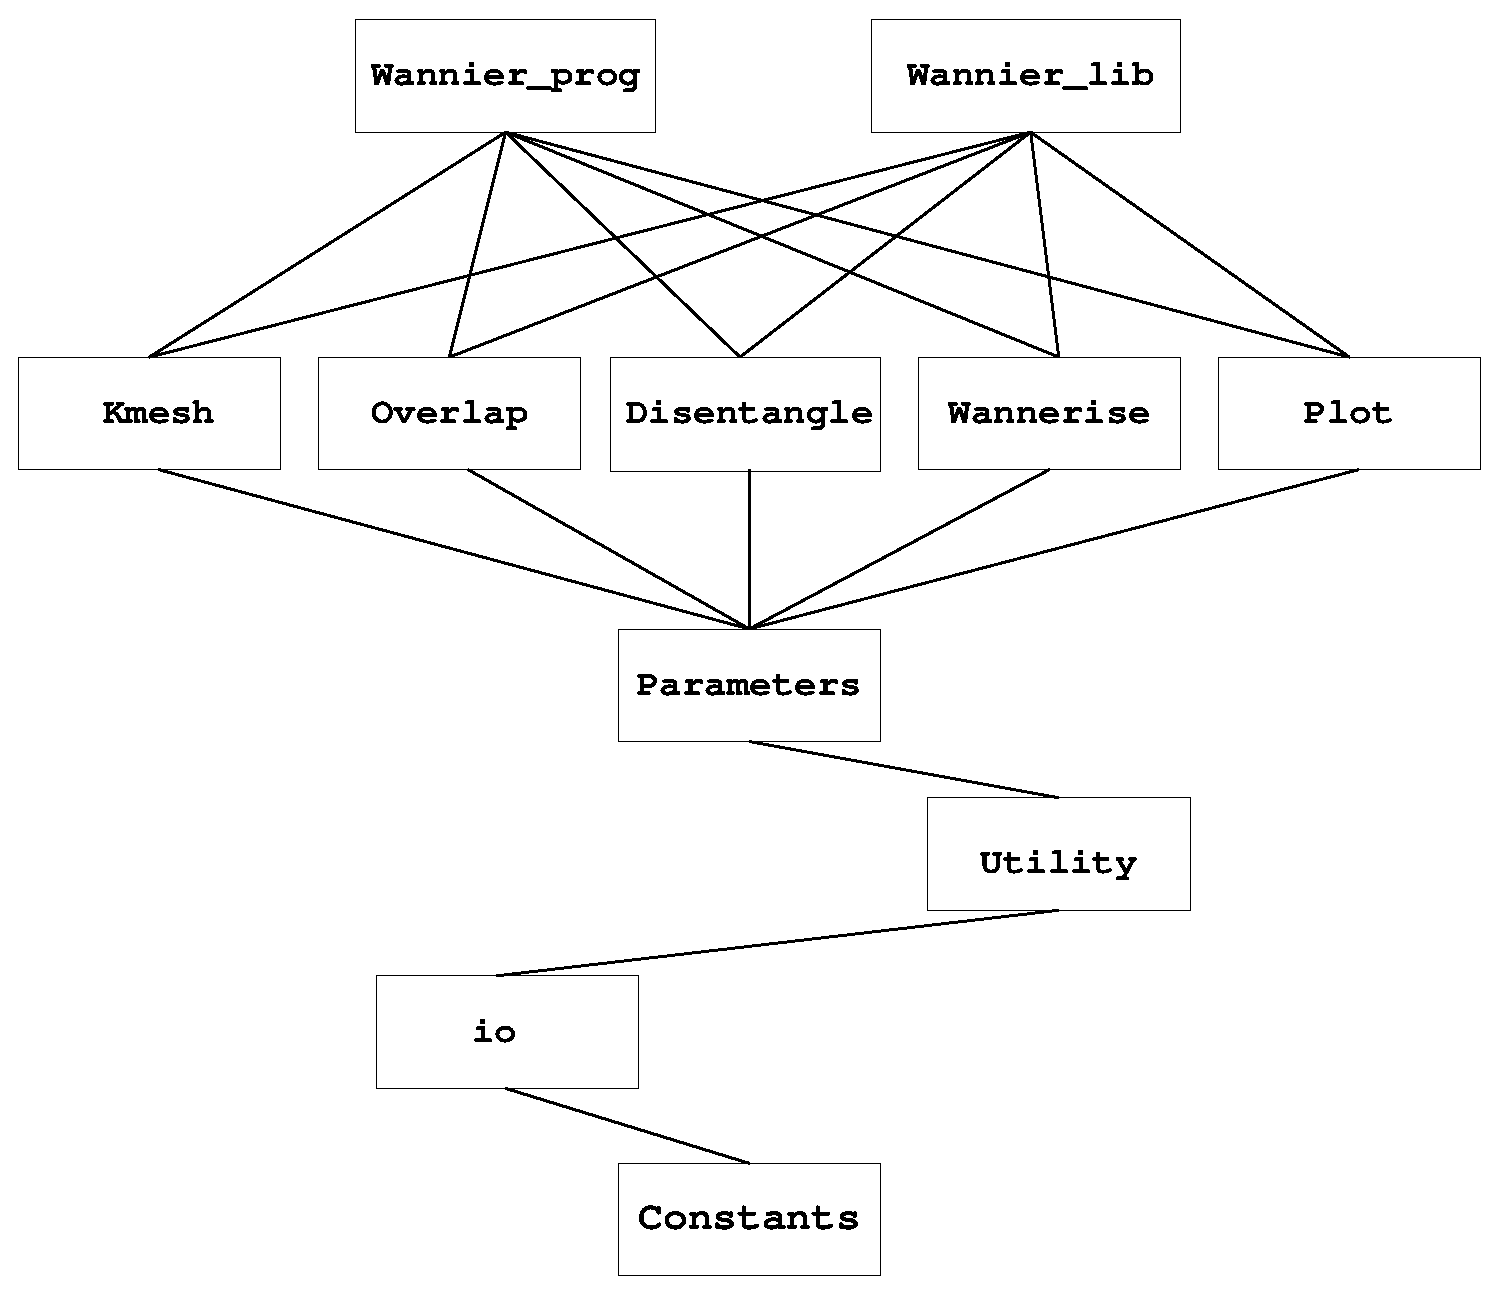
\includegraphics[width=5in]{overview.eps}
\caption{Schematic overview of the module structure of the wannier90 code. Modules may only use data
and subroutines from lower modules.}
\label{structure}
\end{center}
\end{figure}


\chapter{\wannier\ as a post-processing tool} \label{ch:wann-pp}

This is a description of how to use \wannier\ as a
post-processing tool. 

The code must be run twice. On the first pass either the logical
keyword \verb#postproc_setup# must be set to \verb#.true.# in the
input file \verb#seedname.win# or the code must be run with the
command line option \verb#-pp#.  Running the code then generates the
file \verb#seedname.nnkp# which provides the information required to
construct the $M_{mn}^{(\mathbf{k,b})}$ overlaps
(Ref.~\cite{marzari-prb97}, Eq.~(25)) and $A_{mn}^{(\mathbf{k})}$
(Ref.~\cite{marzari-prb97}, Eq.~(62); Ref.~\cite{souza-prb01},
Eq.~(22)).

Once the overlaps and projection have been computed and written to
files \verb#seedname.mmn# and \verb#seedname.amn#, respectively,
set \verb#postproc_setup# to \verb#.false.# and run the code. Output is
written to the file \verb#seedname.wout#.


\section{{\tt seedname.nnkp} file}

OUTPUT, if $\verb#postproc_setup#=\verb#.true.#$

The file \verb#seedname.nnkp# provides the information needed to
determine the required overlap elements $M_{mn}^{(\mathbf{k,b})}$ and
projections $A_{mn}^{(\mathbf{k})}$. It is written automatically when
the code is invoked with the \verb#-pp# command-line option (or when
\verb#postproc_setup=.true.# in \verb#seedname.win#. There should be
no need for the user to edit this file.

Much of the information in \verb#seedname.nnkp# is arranged in blocks
delimited by the strings \verb#begin block_name# \ldots
\verb#end block_name#, as described below. 


\subsection{Keywords}
The first line of the file is a user comment, e.g., the date and time:

\verb#File written on 12Feb2006 at 15:13:12#

\noindent 
The only logical keyword is \verb#calc_only_A#, eg,

\verb#calc_only_A  :  F#

\subsection{{\tt Real\_lattice} block}
\begin{verbatim}
begin real_lattice
 2.250000   0.000000   0.000000
 0.000000   2.250000   0.000000
 0.000000   0.000000   2.250000
end real_lattice
\end{verbatim}

The real lattice vectors in units of Angstrom.


\subsection{{\tt Recip\_lattice} block}
\begin{verbatim}
begin recip_lattice
 2.792527   0.000000   0.000000
 0.000000   2.792527   0.000000
 0.000000   0.000000   2.792527
end recip_lattice
\end{verbatim}

The reciprocal lattice vectors in units of inverse Angstrom.


\subsection{{\tt Kpoints} block}
\begin{verbatim}
begin kpoints
  8
  0.00000   0.00000   0.00000
  0.00000   0.50000   0.00000
  .
  .
  .
  0.50000   0.50000   0.50000
end kpoints
\end{verbatim}

The first line in the block is the total number of k-points
\verb#num_kpts#. The subsequent \verb#num_kpts# lines specify the
k-points in crystallographic co-ordinates relative to the reciprocal
lattice vectors.


\subsection{{\tt Projections} block}
\begin{verbatim}
begin projections
   n_proj
   centre   l  mr  r   
     z-axis   x-axis   zona
   centre   l  mr  r   
     z-axis   x-axis   zona
   .
   .
end projections
\end{verbatim}

\noindent
Notes:

\verb#n_proj#: integer; the number of projection centres, equal to the
number of MLWF \verb#num_wann#.

\verb#centre#: three real numbers; projection function centre
in crystallographic co-ordinates relative to the direct lattice
vectors.

\verb#l  mr  r#: three integers; $l$ and $m_\mathrm{r}$ specify the
angular part $\Theta_{lm_{\mathrm{r}}}(\theta,\varphi)$, and
$\mathrm{r}$ specifies the radial part $R_{\mathrm{r}}(r)$ of the
projection function (see Tables~\ref{tab:angular}, \ref{tab:hybrids}
and \ref{tab:radial}). 

\verb#z-axis#: three real numbers; default is
\verb#0.0 0.0 1.0#; defines the axis from which the polar angle
$\theta$ in spherical polar coordinates is measured.

\verb#x-axis#: three real numbers; must be orthogonal to
\verb#z-axis#; default is \verb#1.0 0.0 0.0# or a vector
perpendicular to \verb#z-axis# if \verb#z-axis# is given; defines the
axis from with the azimuthal angle $\varphi$ in spherical polar
coordinates is measured.

\verb#zona#: real number; the value of $\frac{Z}{a}$ associated
with the radial part of the atomic orbital. Units are in reciprocal
Angstrom.

%%\verb#box-size#: real number; the linear dimension of the real-space
%%box (or sphere) for calculating the overlap
%%$\langle\psi_{m\mathbf{k}}|\phi_{n}\rangle$ of a wavefunction with the
%%localised projection function. Units are in Angstrom. This feature is not
%%currently used.


\subsection{{\tt spinor\_projections} block}
\begin{verbatim}
begin spinor_projections
   n_proj
   centre   l  mr  r   
    z-axis   x-axis   zona
     spin spn_quant
   centre   l  mr  r   
    z-axis   x-axis   zona
     spin spn_quant
   .
   .
end spinor_projections
\end{verbatim}

\noindent
Notes: Only one of projections and spinor\_projections should be
defined. Variables are the same as the projections block with the
addition of \verb#spin# and \verb#spn_quant#.

\verb#spin#: integer. `1' or `-1' to denote projection onto up or
down states.

\verb#spn_quant#: three real numbers. Defines the spin quantisation
axis in Cartesian coordinates.



\subsection{{\tt nnkpts} block}
\begin{verbatim}
begin nnkpts
  10
  1   2   0  0  0
  .
  .
end nnkpts
\end{verbatim}

First line: \verb#nntot#, the number of nearest neighbours belonging
to each k-point of the Monkhorst-Pack mesh

Subsequent lines: \verb#nntot#$\times$\verb#num_kpts#
lines, ie, \verb#nntot# lines of data for each k-point of the mesh. 

Each line of consists of 5 integers. The first is the
k-point number \verb#nkp#. The second to the fifth specify it's nearest
neighbours $\mathbf{k+b}$: the second integer points to the k-point
that is the periodic image of the $\mathbf{k+b}$ that we want; the
last three integers give the G-vector, in reciprocal lattice units,
that brings the k-point specified by the second integer (which is in
the first BZ) to the actual $\mathbf{k+b}$ that we need.


\subsection{{\tt exclude\_bands} block}
\begin{verbatim}
begin exclude_bands 
  8 
  1 
  2 
  .
  .
end exclude_bands
\end{verbatim}
To exclude bands (independent of k-point) from the calculation of the 
overlap and projection matrices, for example to ignore shallow-core states.
The first line is the number of states to exclude, the following lines give
the states for be excluded.


\subsection{An example of projections}\label{sec:proj_example}

As a concrete example: one wishes to have a set of four sp$^3$ projection
orbitals on, say, a carbon atom at (0.5,0.5,0.5) in fractional
co-ordinates relative to the direct lattice vectors. In this case
\verb#seedname.win# will contain the following lines:

\begin{verbatim}
begin projections
 C:l=-1
end projections
\end{verbatim}

and \verb#seedname.nnkp#, generated on the first pass of
\wannier\ (with \verb#postproc_setup=T#), will contain: 

\begin{verbatim}
begin projections
   4
   0.50000    0.50000    0.50000    -1  1  1
     0.000  0.000  1.000   1.000  0.000  0.000   2.00 
   0.50000    0.50000    0.50000    -1  2  1
     0.000  0.000  1.000   1.000  0.000  0.000   2.00 
   0.50000    0.50000    0.50000    -1  3  1
     0.000  0.000  1.000   1.000  0.000  0.000   2.00 
   0.50000    0.50000    0.50000    -1  4  1
     0.000  0.000  1.000   1.000  0.000  0.000   2.00 
end projections
\end{verbatim}

where the first line tells us that in total four projections are
specified, and the subsquent lines provide the projection centre, the
angular and radial parts of the orbital (see
Section~\ref{sec:orbital-defs} for definitions), the $z$ and $x$ axes,
and the diffusivity and cut-off radius for the projection orbital.

\textsc{pwscf}, or any other \textit{ab initio} electronic structure
code, then reads \verb#seedname.nnkp# file, calculates the projections
and writes them to \verb#seedname.amn#. 


\section{{\tt seedname.mmn} file} 

INPUT. 

The file \verb#seedname.mmn# contains the overlaps
$M_{mn}^{(\mathbf{k,b})}$.

First line: a user comment, e.g., the date and time

Second line: 3 integers: \verb#num_bands#, \verb#num_kpts#,
\verb#nntot#

Then: $\verb#num_kpts#\times\verb#nntot#$ blocks of data:
 
First line of each block: 5 integers. The first specifies the
$\mathbf{k}$ (i.e., gives the ordinal corresponding to its position in
the list  of k-points in \verb#seedname.win#). The 2nd to 5th integers
specify $\mathbf{k+b}$. The  2nd integer, in particular, points to the
k-point on the list that is a  periodic image of $\mathbf{k+b}$, and
in particular is the image that is actually mentioned in the list. The 
last three integers specify the $\mathbf{G}$ vector, in  reciprocal
lattice units, that brings the k-point specified by the second
integer, and that thus lives inside the first BZ zone, to the actual
$\mathbf{k+b}$ that we need.

Subsequent $\verb#num_bands#\times\verb#num_bands#$ lines of each
block: two real numbers per line. These are the real and imaginary
parts, respectively, of the actual scalar product
$M_{mn}^{(\mathbf{k,b})}$ for $m,n \in [1,\verb#num_bands#]$. The
order of these elements is such that the first index $m$ is fastest.


\section{{\tt seedname.amn} file}

INPUT.

The file \verb#seedname.amn# contains the projection
$A_{mn}^{(\mathbf{k})}$.

First line: a user comment, e.g., the date and time

%Second line: a single integer, either 0 or 1. See below for explanation.

Second line: 3 integers: \verb#num_bands#, \verb#num_kpts#, \verb#num_wann#

                                     
Subsequently
$\verb#num_bands#\times\verb#num_wann#\times\verb#num_kpts#$ 
lines: 3 integers and 2 real numbers on each line. The first 
two integers are the band indices $m$ and $n$. The third integer specifies
the $\mathbf{k}$ by giving the ordinal corresponding to its position
in the list of $k$-points in \verb#seedname.win#. The real numbers
are the real and imaginary parts, respectively, of the actual
$A_{mn}^{(\mathbf{k})}$.

%The flag in the second line of \verb#seedname.amn# is present in order
%to give the \textit{ab initio} code some freedom to choose the shape
%of the projections itself. There are two possibilities:
%\begin{itemize}
%\item If it is 0, then
%\verb#wannier90# assumes that the projections in \verb#seedname.amn#
%have been calculated as specified in \verb#seedname.nnkp# and proceeds
%(if hybrid orbitals are required) to mix them in the correct manner to
%obtain projections onto the desired orbitals specified in
%\verb#seedname.win#
%\item If it is 1, then \verb#wannier90# ignores the specification of
%  the projection orbital shapes in \verb#seedname.win# and takes the
%  \verb#seedname.amn# file `as is', i.e., does no mixing.
%\end{itemize}

%In terms of the example of Section~\ref{sec:proj_example}, let us
%suppose that this flag is set to 0. Then 
%\verb#seedname.amn# contains the overlaps of a wavefunction
%$\psi_{m\mathbf{k}}$ with an atomic s and three p-orbitals
%$\{\verb#s#,\verb#px#,\verb#py#,\verb#pz#\}$.
%\verb#wannier90# will read 
%\verb#seedname.amn# and calculate the projection
%$A_{mn}^{(\mathbf{k})}$ of a $\psi_{m\mathbf{k}}$ onto
%four sp$^3$ orbitals  $\{\phi_{n}\}$ (specified in \verb#seedname.win# by
%\verb#l=-1#, or the string \verb#sp3#)
%by linear mixing as follows:  

%\begin{eqnarray}
%A_{mn}^{(\mathbf{k})} & = & \langle\psi_{m\mathbf{k}}|\phi_{n}\rangle
%                      \nonumber \\
%                      & = &
%                      \langle\psi_{m\mathbf{k}}|\verb#sp3-n#\rangle
%                      \nonumber \\ 
%                      & = &
% \frac{1}{2}\left[\langle\psi_{m\mathbf{k}}|\verb#s#\rangle \pm
% \langle\psi_{m\mathbf{k}}|\verb#px#\rangle \pm
% \langle\psi_{m\mathbf{k}}|\verb#py#\rangle \pm
% \langle\psi_{m\mathbf{k}}|\verb#pz#\rangle\right], \label{eq:Amn}
%\end{eqnarray} 
%
%where the matrix elements on the right-hand side are taken from
%\verb#seedname.amn#. Projections corresponding to four sp$^{3}$
%orbitals \verb#sp3-1#, \verb#sp3-2#, \verb#sp3-3#, and \verb#sp3-4# --
%see Section~\ref{sec:orbital-defs} -- are
%obtained with appropriate choice of the signs in Eq.~(\ref{eq:Amn}): 
%($+$,$+$,$+$), ($+$,$-$,$-$), ($-$,$+$,$-$) and
%($-$,$-$,$+$).


\section{{\tt seedname.eig} file}

INPUT. 

Required if any of \verb#disentanglement#, \verb#plot_bands#,
   \verb#plot_fermi_surface# or \verb#hr_plot# are \verb#.true.#

The file \verb#seedname.eig# contains the Kohn-Sham eigenvalues
     $\varepsilon_{n\mathbf{k}}$ (in eV) at each point in the
     Monkhorst-Pack mesh.

Each line consist of two integers and a real number. The first integer
is the band index, the second integer gives the ordinal corresponding
to the $k$-point in the list of $k$-points in \verb#seedname.win#,
and the real number is the eigenvalue. 

E.g.,

\begin{verbatim}
           1           1  -6.43858831271328
           2           1   19.3977795287297
           3           1   19.3977795287297
           4           1   19.3977795287298
\end{verbatim}


\section{Interface with {\sc pwscf}}

Interfaces between \wannier\ and many ab-initio codes as \pwscf, 
{\sc abinit} (\url{http://www.abinit.org}),
{\sc siesta} (\url{http://www.icmab.es/siesta/}), 
{\sc fleur}, {\sc VASP} and {\sc Wien2k} (\url{http://www.wien2k.at}) are
available.  Here we describe the
seamless interface between \wannier\ and \pwscf, a
plane-wave DFT code that comes as part of the {\sc Quantum ESPRESSO}
package (see \url{http://www.quantum-espresso.org}).
You will need
to download and compile \pwscf\ (i.e., the {\tt pw.x} code) and the
post-processing interface {\tt pw2wannier90.x}. Please refer to the
documentation that comes with the {\sc Quantum ESPRESSO} distribution
for instructions. 

\begin{enumerate}
\item Run `scf'/`nscf' calculation(s) with \verb#pw#
\item Run \wannier\ with \verb#postproc_setup#~=~\verb#.true.# to
  generate \verb#seedname.nnkp#
\item Run {\tt pw2wannier90}. First it reads an input file, e.g.,
  \verb#seedname.pw2wan#, which defines \verb#prefix# and
  \verb#outdir# for the underlying `scf' calculation, as well as the
  name of the file \verb#seedname.nnkp#, and does a consistency check
  between the direct and reciprocal lattice vectors read from
  \verb#seedname.nnkp# and those defined in the files specified by
  \verb#prefix#. \verb#pw2wannier90# generates \verb#seedname.mmn#,
  \verb#seedname.amn# and \verb#seedname.eig# 
\item Run \verb#wannier90# with \verb#postproc_setup#~=~\verb#.false.# to
  disentangle bands (if required), localise MLWF, and use MLWF for
  plotting, bandstructures, Fermi surfaces etc.
\end{enumerate}

Examples of how the interface with \pwscf\ works are given in the
\wannier\ Tutorial. 

\subsection{{\tt seedname.pw2wan}}

A number of keywords may be specified in the {\tt pw2wannier90} input file:


\begin{itemize}

\item   \verb#outdir# -- Location to write output files. Default is \verb#`./'#

\item   \verb#prefix# -- Prefix for the \pwscf\ calculation. Default is \verb#` '#

\item   \verb#seedname# -- Seedname for the \wannier\ calculation. Default
   is \verb#`wannier'#

\item   \verb#spin_component# -- Spin component. Takes values \verb#`up'#,
   \verb#`down'# or \verb#`none'# (default).

\item   \verb#wan_mode# -- Either \verb#`standalone'# (default) or \verb#`library'#

\item   \verb#write_unk# -- Set to \verb#.true.# to write the periodic part
   of the Bloch functions for plotting in \wannier. Default is
   \verb#.false.#

\item   \verb#reduce_unk# -- Set to \verb#.true.# to reduce file-size (and
   resolution) of Bloch functions by a factor of 8. Default is
   \verb#.false.# (only relevant if
   \verb#write_unk=.true.#)\footnote{Note that there is a small bug
   with this feature in v3.2 (and subsequent patches) of {\tt
   quantum-espresso}. Please use a later version (if available) or the
   CVS version of {\tt pw2wannier90.f90}, which has been fixed.}

\item   \verb#wvfn_formatted# -- Set to \verb#.true.# to write formatted
   wavefunctions. Default is \verb#.false.# (only relevant if
   \verb#write_unk=.true.#)

\item   \verb#write_amn# -- Set to \verb#.false.# if
   $A_{mn}^{(\mathbf{k})}$ not required. Default is \verb#.true.#

\item   \verb#write_mmn# -- Set to \verb#.false.# if
   $M_{mn}^{(\mathbf{k,b})}$ not required. Default is \verb#.true.#

\item   \verb#write_spn# -- Set to \verb#.true.# to write out the matrix
   elements of $S$ between Bloch states (non-collinear spin calculation
   only). Default is \verb#.false.#

\item   \verb#spn_formatted# -- Set to \verb#.true.# to write spn data as a formatted file. Default is \verb#.false.# (only relevant if
   \verb#write_spn=.true.#)


\item   \verb#write_uHu# -- Set to \verb#.true.# to write out the matrix
   elements $$\langle u_{n{\bf k}+{\bf b}_1}\vert
H_{\bf k}\vert u_{m{\bf k}+{\bf b}_2}\rangle.
$$
Default is \verb#.false.#

\item   \verb#uHu_formatted# -- Set to \verb#.true.# to write uHu data as a formatted file. Default is \verb#.false.# (only relevant if
   \verb#write_uHu=.true.#)


\item   \verb#write_uIu# -- Set to \verb#.true.# to write out the matrix
   elements of $$\langle  u_{n{\bf k}+{\bf b}_1}\vert
u_{m{\bf k}+{\bf b}_2}\rangle.
$$ Default is \verb#.false.# 

\item   \verb#uIu_formatted# -- Set to \verb#.true.# to write uIu data as a formatted file. Default is \verb#.false.# (only relevant if
   \verb#write_uIu=.true.#)



\item   \verb#write_unkg# -- Set to \verb#.true.# to write the first few
   Fourier components of the periodic parts of the Bloch functions.



\end{itemize}

For examples of use, refer to the \wannier\ Tutorial.


%!TEX root=./user_guide.tex
\chapter{\wannier\ as a library}\label{ch:wann-lib}

This is a description of the interface between any external program
and the wannier code. There are two subroutines: \verb#wannier_setup#
and \verb#wannier_run#. Calling \verb#wannier_setup# will return
information required to construct the $M_{mn}^{(\mathbf{k,b})}$
overlaps (Ref.~\cite{marzari-prb97}, Eq.~(25)) and
$A_{mn}^{(\mathbf{k})}=\left\langle
  \psi_{m\mathbf{k}}|g_{n}\right\rangle$ projections
(Ref.~\cite{marzari-prb97}, Eq.~(62); Ref.~\cite{souza-prb01},
Eq.~(22)). Once the overlaps and projection have been computed,
calling \verb#wannier_run# activates the minimisation and plotting
routines in \wannier.

\textbf{IMPORTANT NOTE:} the library mode ONLY works in serial. Please
call it from a serial code, or if compiled in parallel, make sure to run
it from a single MPI process.

You can find a minimal example of how the library mode can be used
among the tests, in the file 
\verb|test-suite/library-mode-test/test_library.F90| 
in the Wannier90 git repository.

%\section{Dependencies}
%\begin{itemize}
%\item Parameters
%\item IO
%\item Kmesh
%\item Overlap
%\item Wannierise
%\end{itemize}

\section{Subroutines}

\subsection{{\tt wannier\_setup}}

{\noindent \bf \verb#wannier_setup(seed_name,mp_grid,num_kpts,real_lattice,recip_lattice,#\\
\verb#              kpt_latt,num_bands_tot,num_atoms,atom_symbols,atoms_cart,#\\
\verb#              gamma_only,spinors,nntot,nnlist,nncell,num_bands,num_wann,proj_site,#\\
\verb#              proj_l,proj_m,proj_radial,proj_z,proj_x,proj_zona,#\\
\verb#              exclude_bands,proj_s,proj_s_qaxis)#}

\begin{itemize}
\item \verb#character(len=*), intent(in) :: seed_name#\\ The seedname
  of the current calculation.
\item \verb#integer, dimension(3), intent(in) :: mp_grid#\\ The
  dimensions of the {Monkhorst-Pack} k-point grid.
\item \verb#integer, intent(in) :: num_kpts#\\ The number of k-points on
  the {Monkhorst-Pack} grid.
\item \verb#real(kind=dp), dimension(3,3), intent(in) :: real_lattice#\\
  The lattice vectors in Cartesian co-ordinates in units of Angstrom.
\item \verb#real(kind=dp), dimension(3,3), intent(in) :: recip_lattice#\\
  The reciprocal lattice vectors in Cartesian co-ordinates in units of reciprocal Angstrom.
\item
  \verb#real(kind=dp), dimension(3,num_kpts), intent(in) :: kpt_latt#\\
  The positions of the k-points in fractional co-ordinates
  relative to the reciprocal lattice vectors.
\item \verb#integer, intent(in) :: num_bands_tot#\\ The total number of bands in the
first-principles calculation (note: including semi-core states).
\item \verb#integer, intent(in) :: num_atoms#\\ The total number of atoms
  in the system.
\item \verb#character(len=20), dimension(num_atoms),#
      \verb# intent(in) :: atom_symbols#\\ The elemental symbols of
      the atoms.
\item \verb#real(kind=dp), dimension(3,num_atoms),#
      \verb#intent(in) :: atoms_cart#\\ The positions of the atoms in
      Cartesian co-ordinates in Angstrom.
\item \verb#logical, intent(in) :: gamma_only#\\ Set to \texttt{.true.} if the
  underlying electronic structure calculation has been performed with
  only $\Gamma$-point sampling and, hence, if the Bloch eigenstates
  that are used to construct $A_{mn}^{(\mathbf{k})}$ and
  $M_{mn}^{\mathbf{(k,b)}}$ are real.
\item \verb#logical, intent(in) :: spinors#\\ Set to \texttt{.true.} if
  underlying electronic structure calculation has been performed with
  spinor wavefunctions. 
\item \verb#integer, intent(out) :: nntot#\\ The
  total number of nearest neighbours for each k-point. 
\item \verb#integer, dimension(num_kpts,num_nnmax),#
      \verb# intent(out) :: nnlist#\\
      The list of nearest neighbours for each k-point.
\item \verb#integer,dimension(3,num_kpts,num_nnmax),#
      \verb# intent(out) :: nncell#\\ 
      The vector, in fractional reciprocal lattice co-ordinates, that
      brings the \verb#nn#$^{\mathrm{th}}$ nearest neighbour of
      k-point \verb#nkp# to its periodic image that
      is needed for computing the overlap 
      $M_{mn}^{(\mathbf{k,b})}$.
\item \verb#integer, intent(out) :: num_bands#\\ The number of bands in the
first-principles calculation used to form the overlap matricies (note: excluding eg. semi-core states).
\item \verb#integer, intent(out) :: num_wann#\\ The number of MLWF
  to be extracted.
\item  \verb#real(kind=dp), dimension(3,num_bands_tot), intent(out) :: proj_site# \\
Projection function centre
in crystallographic co-ordinates relative to the direct lattice
vectors.
\item \verb#integer, dimension(num_bands_tot), intent(out) :: proj_l#\\
 $l$  specifies the angular part $\Theta_{lm_{\mathrm{r}}}(\theta,\varphi)$ of the
projection function  (see Tables~\ref{tab:angular}, \ref{tab:hybrids}
and \ref{tab:radial}). 
\item \verb#integer, dimension(num_bands_tot), intent(out) :: proj_m#\\
 $m_\mathrm{r}$ specifies the angular part $\Theta_{lm_{\mathrm{r}}}(\theta,\varphi)$, of the
projection function
 (see Tables~\ref{tab:angular}, \ref{tab:hybrids}
and \ref{tab:radial}). 
\item \verb#integer, dimension(num_bands_tot), intent(out) :: proj_radial#\\
$\mathrm{r}$ specifies the radial part $R_{\mathrm{r}}(r)$ of the
projection function 
(see Tables~\ref{tab:angular}, \ref{tab:hybrids}
and \ref{tab:radial}). 
\item  \verb#real(kind=dp), dimension(3,num_bands_tot), intent(out) :: proj_z#\\
Defines the axis from which the polar angle
$\theta$ in spherical polar coordinates is measured. Default is
\verb#0.0 0.0 1.0#.
\item  \verb#real(kind=dp), dimension(3,num_bands_tot), intent(out) :: proj_x#\\
Must be orthogonal to
\verb#z-axis#; default is \verb#1.0 0.0 0.0# or a vector
perpendicular to \verb#proj_z# if \verb#proj_z# is given; defines the
axis from with the azimuthal angle $\varphi$ in spherical polar
coordinates is measured.
\item \verb#real(kind=dp), dimension(num_bands_tot), intent(out) :: proj_zona#\\
The value of $\frac{Z}{a}$ associated
with the radial part of the atomic orbital. Units are in reciprocal
Angstrom.
\item \verb#integer, dimension(num_bands_tot), intent(out) :: exclude_bands#\\ 
      Kpoints independant list of bands to exclude from the
      calculation of the MLWF (e.g., semi-core states). 
\item \verb#integer, dimension(num_bands_tot), optional,intent(out) :: proj_s#\\
'1' or '-1' to denote projection onto up or down spin states
\item  \verb#real(kind=dp), dimension(3,num_bands_tot), intent(out) :: proj_s_qaxisx#\\
Defines the spin quantisation axis in Cartesian coordinates.

\end{itemize}

Conditions:
\begin{itemize}
\cond $\verb#num_kpts# = \verb#mp_grid(1)# \times \verb#mp_grid(2)#
\times \verb#mp_grid(3)#$.
\cond $\verb#num_nnmax# = 12$
\end{itemize}

This subroutine returns the information required to determine the
required overlap elements $M_{mn}^{(\mathbf{k,b})}$ and
projections $A_{mn}^{(\mathbf{k})}$,
i.e., \verb#M_matrix# and \verb#A_matrix#, described in
Section~\ref{wannier_run}. 

For the avoidance of doubt, \verb#real_lattice(1,2)# is the
$y-$component of the first lattice vector $\mathbf{A}_{1}$, etc.

The list of nearest neighbours of a particular k-point \verb#nkp# is
given by \verb#nnlist(nkp,1:nntot)#.

Additionally, the parameter \verb#shell_list#
may be specified in the \wannier\ input file.

\subsection{{\tt wannier\_run}} \label{wannier_run}

{\noindent \bf \verb#wannier_run(seed_name,mp_grid,num_kpts,real_lattice,recip_lattice,#\\
\verb#            kpt_latt,num_bands,num_wann,nntot,num_atoms,atom_symbols,#\\
\verb#            atoms_cart,gamma_only,M_matrix_orig,A_matrix,eigenvalues,#\\
\verb#            U_matrix,U_matrix_opt,lwindow,wann_centres,wann_spreads,#\\
\verb#            spread#)}

\begin{itemize}
\item \verb#character(len=*), intent(in) :: seed_name#\\ The seedname
  of the current calculation.
\item \verb#integer, dimension(3), intent(in) :: mp_grid#\\ The
  dimensions of the {Monkhorst-Pack} k-point grid.
\item \verb#integer, intent(in) :: num_kpts#\\ The number of k-points on
  the {Monkhorst-Pack} grid.
\item \verb#real(kind=dp), dimension(3,3),#
      \verb# intent(in) :: real_lattice#\\ The lattice vectors in
      Cartesian co-ordinates in units of Angstrom. 
\item \verb#real(kind=dp), dimension(3,3), intent(in) :: recip_lattice#\\
  The reciprical lattice vectors in Cartesian co-ordinates in units of inverse Angstrom.
\item \verb#real(kind=dp), dimension(3,num_kpts),#
      \verb# intent(in) :: kpt_latt#\\ The positions of the k-points in
      fractional co-ordinates relative to the reciprocal lattice
      vectors.
\item \verb#integer, intent(in) :: num_bands#\\ The total number of
      bands to be processed.
\item \verb#integer, intent(in) :: num_wann#\\ The number of MLWF to
  be extracted. 
\item \verb#integer, intent(in) :: nntot#\\ The number of
  nearest neighbours for each k-point.
\item \verb#integer, intent(in) :: num_atoms#\\ The total number of atoms
  in the system.
\item \verb#character(len=20), dimension(num_atoms),#
      \verb# intent(in) :: atom_symbols#\\ The elemental symbols of
      the atoms.
\item \verb#real(kind=dp), dimension(3,num_atoms),#
      \verb#intent(in) :: atoms_cart#\\ The positions of the atoms in
      Cartesian co-ordinates in Angstrom.
\item \verb#logical, intent(in) :: gamma_only#\\ Set to \texttt{.true.} if the
  underlying electronic structure calculation has been performed with
  only $\Gamma$-point sampling and, hence, if the Bloch eigenstates
  that are used to construct $A_{mn}^{(\mathbf{k})}$ and
  $M_{mn}^{\mathbf{(k,b)}}$ are real.
\item \verb#complex(kind=dp),#
      \verb# dimension(num_bands,num_bands,nntot,num_kpts),#\\
      \verb#                  intent(in) :: M_matrix#\\ 
      The matrices of overlaps between neighbouring periodic parts of
      the Bloch eigenstates at each k-point, $M_{mn}^{(\mathbf{(k,b)})}$
      (Ref.~\cite{marzari-prb97}, Eq.~(25)).
\item \verb#complex(kind=dp), dimension(num_bands,num_wann,num_kpts),#\\
      \verb#                  intent(in) :: A_matrix# \\The matrices
      describing the projection of \verb#num_wann# trial orbitals on
      \verb#num_bands# Bloch states at each k-point,
      $A_{mn}^{(\mathbf{k})}$ (Ref.~\cite{marzari-prb97}, Eq.~(62);
      Ref.~\cite{souza-prb01}, Eq.~(22)).
\item \verb#real(kind=dp), dimension(num_bands,num_kpts),#
      \verb#intent(in) :: eigenvalues#\\ The
      eigenvalues $\varepsilon_{n\mathbf{k}}$ corresponding to the
      eigenstates, in eV.
\item \verb#complex(kind=dp), dimension(num_wann,num_wann,num_kpts),#\\
      \verb#                  intent(out) :: U_matrix#\\ The unitary
      matrices at each k-point (Ref.~\cite{marzari-prb97}, Eq.~(59))
\item \verb#complex(kind=dp), dimension(num_bands,num_wann,num_kpts),#\\
      \verb#               optional, intent(out) :: U_matrix_opt#\\ The
      unitary matrices that describe the optimal sub-space at each
      k-point (see Ref.~\cite{souza-prb01}, Section~{\sc IIIa}). The array is
      packed (see below) 
\item \verb#logical, dimension(num_bands,num_kpts), optional, intent(out) :: lwindow#\\ 
       The element \verb#lwindow(nband,nkpt)# is {\tt .true.} if the band
{\tt nband} lies within the outer energy window at kpoint {\tt nkpt}.
\item \verb#real(kind=dp), dimension(3,num_wann), optional, intent(out) :: wann_centres#\\   
      The centres of the MLWF in Cartesian co-ordinates in Angstrom. 
\item \verb#real(kind=dp), dimension(num_wann), optional, intent(out) :: wann_spreads#\\ 
      The spread of each MLWF in \AA$^{2}$.
\item \verb#real(kind=dp), dimension(3), optional, intent(out) ::#
      \verb#spread#\\ 
      The values of $\Omega$, $\Omega_{\mathrm{I}}$ and
      $\tilde{\Omega}$ (Ref.~\cite{marzari-prb97}, Eq.~(13)). 
\end{itemize}

Conditions:
\begin{itemize}
\cond $\verb#num_wann# \le \verb#num_bands#$
\cond $\verb#num_kpts# = \verb#mp_grid(1)# \times \verb#mp_grid(2)#
\times \verb#mp_grid(3)#$.
\end{itemize}

If $\verb#num_bands# = \verb#num_wann#$ then \verb#U_matrix_opt# is the identity matrix and
\verb#lwindow=.true.#

For the avoidance of doubt, \verb#real_lattice(1,2)# is the
$y-$component of the first lattice 
vector $\mathbf{A}_{1}$, etc.

\begin{eqnarray*}
\verb#M_matrix(m,n,nn,nkp)# & = & \left\langle u_{m\mathbf{k}} |
u_{n\mathbf{k+b}}\right\rangle\\
\verb#A_matrix(m,n,nkp)# & = &
\left\langle \psi_{m\mathbf{k}}|g_{n}\right\rangle\\
\verb#eigenvalues(n,nkp)# &=& \varepsilon_{n\mathbf{k}}
\end{eqnarray*}
where
\begin{eqnarray*}
\mathbf{k} &=&\verb#kpt_latt(1:3,nkp)#\\
\mathbf{k+b}&=& \verb#kpt_latt(1:3,nnlist(nkp,nn))# +
\verb#nncell(1:3,nkp,nn)# 
\end{eqnarray*}
and
$\left\{|g_{n}\rangle\right\}$ are a set of initial trial
orbitals. These are
typically atom or bond-centred Gaussians that are modulated by
appropriate spherical harmonics. 

Additional parameters should be specified in the \wannier\ input
file.



\chapter{Transport Calculations with \wannier\ }\label{ch:transport}

By setting $\verb#transport#=\verb#TRUE#$, \wannier\ will calculate
the quantum conductance and density of states of a one-dimensional
system. The results will be written to files \verb#seedname_qc.dat#
and \verb#seedname_dos.dat#, respectively.

The system for which transport properties are calculated is determined
by the keyword \verb#transport_mode#.

\section{\tt transport\_mode = bulk}

Quantum conductance and density of states are calculated for a perfectly
periodic one-dimensional conductor. If $\verb#tran_read_ht#=\verb#FALSE#$
the transport properties are calculated using the Hamiltonian in the Wannier 
function basis of the system found by \wannier. Setting 
$\verb#tran_read_ht#=\verb#TRUE#$ allows the user to provide an 
external Hamiltonian matrix file {\tt seedname\_htB.dat}, from which
the properties are found. See Section~\ref{sec:post-p} for more details of 
the keywords required for such calculations.

\section{\tt transport\_mode = lcr}

Quantum conductance and density of states are calculated 
for a system where semi-infinite, left and right leads
are connected through a central conductor region. This is known 
as the \emph{lcr} system.
Details of the method is described in Ref. \cite{Nardelli}.

In \wannier\ two options exist for performing such calculations: 
\begin{itemize}
\item If $\verb#tran_read_ht#=\verb#TRUE#$ the external Hamiltonian 
files {\tt seedname\_htL.dat, seedname\_htLC.dat, seedname\_htC.dat, 
seedname\_htCR.dat, seedname\_htR.dat} are read and used to compute 
the transport properties. 
\item If $\verb#tran_read_ht#=\verb#FALSE#$, then the transport
calculation is performed automatically using the Wannier functions as a
basis and the 2c2 geometry described in Section~\ref{sec:2c2}.
\end{itemize}

\section{Automated lcr Transport Calculations: The 2c2 Geometry}
\label{sec:2c2}

Calculations using the 2c2 geometry provide a method to calculate the
transport properties of an lcr system from a single \wannier\ calculation.
The Hamiltonian matrices which the five external files provide in the 
$\verb#tran_read_ht#=\verb#TRUE#$ case are instead built from the 
Wannier function basis directly. As such, strict rules apply to the system geometry, 
which is shown in Figure~\ref{fig:2c2}. These rules are as follows:
\begin{itemize}
\item Left and right leads must be identical and periodic.
\item Supercell must contain two principal layers (PLs) of lead on the left,
a central conductor region and two principal layers of lead on the right.
\item The conductor region must contain enough lead such that the
disorder does not affect the principal layers of lead either side.
\item A single k-point (Gamma) must be used.
\end{itemize}

\begin{figure}[h]
\centering
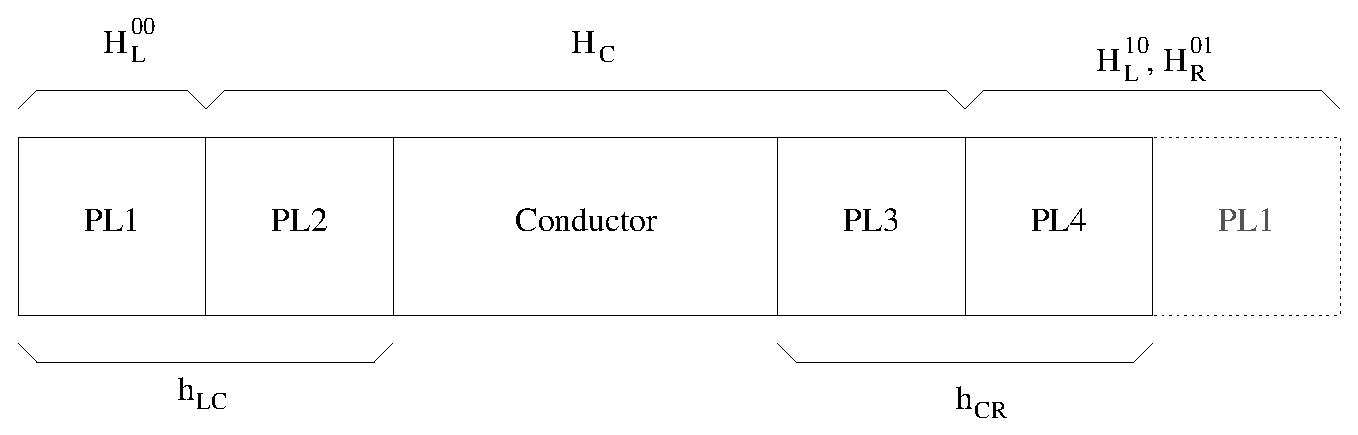
\includegraphics[height=4cm]{lcr_2c2}
\caption{Schematic illustration of the supercell required for 2c2
lcr calculations, showing where each of the Hamiltonian matrices
are derived from. Four principal layers (PLs) are required plus the
conductor region.}
\label{fig:2c2}
\end{figure}

In order to build the Hamiltonians, Wannier  functions are first 
sorted according to position and then consistent parities are enforced.
Therefore the following are also required:
\begin{itemize}
\item The number of Wannier functions in a principal layer, 
\verb#tran_num_ll#.
\item The number of unit cells in one PL of lead
\verb#tran_num_cell_ll#.
\item The \verb#UNKp.s# file.
\end{itemize}

Further parameters related to these calculations are 
\verb#tran_group_threshold# and \verb#tran_wf_threshold#.

Examples of how 2c2 calculations are performed can be found 
in the \wannier\ Tutorial.


\chapter{Files}


\section{{\tt seedname.win}}
INPUT. The master input file; contains the specification of the system
and any parameters for the run. For a description of input parameters,
see Chapter~\ref{chap:parameters}; for examples, see
Section~\ref{winfile} and the \wannier\
Tutorial.

\subsection{Units}

The following are the dimensional quantities that are
specified in the master input file:

\begin{itemize}
\item Direct lattice vectors
\item Positions (of atomic or projection) centres in real space
\item Energy windows
\item Positions of k-points in reciprocal space
\item Convergence thresholds for the minimisation of $\Omega$
%%\item \verb#zona# and \verb#box-size# (see Section~\ref{sec:proj})
\item \verb#zona# (see Section~\ref{sec:proj})
\item \verb#wannier_plot_cube#: cut-off radius for plotting WF in
  Gaussian cube format
\end{itemize}

Notes:

\begin{itemize}
\item The units (either \verb#ang#
  (default) or \verb#bohr#) in which the lattice vectors, atomic
  positions or projection centres are given can be set in the first
  line of the blocks 
  \verb#unit_cell_cart#, \verb#atoms_cart# and \verb#projections#,
  respectively, in \verb#seedname.win#.
\item Energy is always in eV.
\item Convergence thresholds are always in \AA$^{2}$
\item Positions of k-points are always in crystallographic
  coordinates relative to the reciprocal lattice vectors.
%%\item \verb#box-size# and \verb#zona# always in Angstrom and
%%  reciprocal Angstrom, respectively
\item \verb#zona# is always in reciprocal Angstrom (\AA$^{-1}$)
\item The keyword \verb#length_unit# may be set to \verb#ang#
  (default) or \verb#bohr#, in order to set the units in which the
  quantities in the output file {\tt seedname.wout} are written.
\item \verb#wannier_plot_radius# is in Angstrom
\end{itemize}

The reciprocal lattice vectors
$\{\mathbf{B}_{1},\mathbf{B}_{2},\mathbf{B}_{3}\}$ are defined in
terms
of the direct lattice vectors
$\{\mathbf{A}_{1},\mathbf{A}_{2},\mathbf{A}_{3}\}$ by the equation

\begin{equation}
\mathbf{B}_{1} = \frac{2\pi}{\Omega}\mathbf{A}_{2}\times\mathbf{A}_{3}
\ \ \ \mathrm{etc.},
\end{equation}

where the cell volume is
$V=\mathbf{A}_{1}\cdot(\mathbf{A}_{2}\times\mathbf{A}_{3})$.

\section{{\tt seedname.mmn}}
INPUT. Written by the underlying electronic structure code. See
Chapter~\ref{ch:wann-pp} for details.

\section{{\tt seedname.amn}}
INPUT. Written by the underlying electronic structure code. See
Chapter~\ref{ch:wann-pp} for details. 

\section{{\tt seedname.eig}}
INPUT. Written by the underlying electronic structure code. See
Chapter~\ref{ch:wann-pp} for details.

\section{{\tt seedname.nnkp}} \label{sec:old-nnkp}
OUTPUT. Written by \wannier\ when {\tt postproc\_setup=.TRUE.} (or,
alternatively, when \wannier\ is run with the {\tt -pp} command-line
option). See Chapter~\ref{ch:wann-pp} for details.

\section{{\tt seedname.wout}}
OUTPUT. The master output file. Here we give a description of the main
features of the output. The verbosity of the output is controlled by
the input parameter {\tt iprint}. The higher the value, the more
detail is given in the output file. The default value is 1, which prints
minimal information.

\subsection{Header}

The header provides some basic information about \wannier, the
authors, and the execution time of the current run.

\begin{verbatim}

             +---------------------------------------------------+
             |                                                   |
             |                     WANNIER90                     |
             |                                                   |
             +---------------------------------------------------+
             |                                                   |
             |        Welcome to the Maximally-Localized         |
             |        Generalized Wannier Functions code         |
             |            http://www.wannier.org                 |
             |                                                   |
             |  Authors:                                         |
             |    Arash A. Mostofi   (Imperial College London)   |
             |    Jonathan R. Yates  (University of Cambridge)   |
             |    Young-Su Lee       (KIST, S. Korea)            |
             |                                                   |
                                       .
                                       .
             |                                                   |
             |   Copyright (c) 1997-2007 J. Yates, A. Mostofi,   |
             |   Y.-S. Lee, N. Marzari, I. Souza, D. Vanderbilt  |
             |                                                   |
             |          Release: 1.1       1st Sep 2007          |
             |                                                   |
                                       .
                                       .
             |                                                   |
             +---------------------------------------------------+
             |    Execution started on 10Sep2007 at 12:46:57     |
             +---------------------------------------------------+

\end{verbatim}

\subsection{System information}

This part of the output file presents information that \wannier\ has
read or inferred from the master input file {\tt seedname.win}. This
includes real and reciprocal lattice vectors, atomic positions,
k-points, parameters for job control, disentanglement, localisation
and plotting. 

\begin{verbatim}
                                    ------
                                    SYSTEM
                                    ------
 
                              Lattice Vectors (Ang)
                    a_1     3.938486   0.000000   0.000000
                    a_2     0.000000   3.938486   0.000000
                    a_3     0.000000   0.000000   3.938486
 
                   Unit Cell Volume:      61.09251  (Ang^3)
 
                        Reciprocal-Space Vectors (Ang^-1)
                    b_1     1.595330   0.000000   0.000000
                    b_2     0.000000   1.595330   0.000000
                    b_3     0.000000   0.000000   1.595330
  
 *----------------------------------------------------------------------------*
 |   Site       Fractional Coordinate          Cartesian Coordinate (Ang)     |
 +----------------------------------------------------------------------------+
 | Ba   1   0.00000   0.00000   0.00000   |    0.00000   0.00000   0.00000    |
 | Ti   1   0.50000   0.50000   0.50000   |    1.96924   1.96924   1.96924    |
                                          .
                                          . 
 *----------------------------------------------------------------------------*
  
                                ------------
                                K-POINT GRID
                                ------------
  
             Grid size =  4 x  4 x  4      Total points =   64
  
 *---------------------------------- MAIN ------------------------------------*
 |  Number of Wannier Functions               :                 9             |
 |  Number of input Bloch states              :                 9             |
 |  Output verbosity (1=low, 5=high)          :                 1             |
 |  Length Unit                               :               Ang             |
 |  Post-processing setup (write *.nnkp)      :                 F             |
                                              .
                                              .
 *----------------------------------------------------------------------------*
\end{verbatim}

\subsection{Nearest-neighbour k-points}

This part of the output files provides information on the
$\mathrm{b}$-vectors and weights chosen to satisfy the condition of
Eq.~\ref{eq:B1}. 

\begin{verbatim}
 *---------------------------------- K-MESH ----------------------------------*
 +----------------------------------------------------------------------------+
 |                    Distance to Nearest-Neighbour Shells                    |
 |                    ------------------------------------                    |
 |          Shell             Distance (Ang^-1)          Multiplicity         |
 |          -----             -----------------          ------------         |
 |             1                   0.398833                      6            |
 |             2                   0.564034                     12            |
                                       .
                                       .
 +----------------------------------------------------------------------------+
 | The b-vectors are chosen automatically                                     |
 | The following shells are used:   1                                         |
 +----------------------------------------------------------------------------+
 |                        Shell   # Nearest-Neighbours                        |
 |                        -----   --------------------                        |
 |                          1               6                                 |
 +----------------------------------------------------------------------------+
 | Completeness relation is fully satisfied [Eq. (B1), PRB 56, 12847 (1997)]  |
 +----------------------------------------------------------------------------+
\end{verbatim}

\subsection{Disentanglement}

Then (if required) comes the part where $\omi$ is minimised to
disentangle the optimally-connected subspace of states for the
localisation procedure in the next step.

First, a summary of the energy windows that are being used is given:
\begin{verbatim}
 *------------------------------- DISENTANGLE --------------------------------*
 +----------------------------------------------------------------------------+
 |                              Energy  Windows                               |
 |                              ---------------                               |
 |                   Outer:    2.81739  to   38.00000  (eV)                   |
 |                   Inner:    2.81739  to   13.00000  (eV)                   |
 +----------------------------------------------------------------------------+
\end{verbatim}

Then, each step of the iterative minimisation of $\omi$ is reported. 
\begin{verbatim}                                   
                   Extraction of optimally-connected subspace                  
                   ------------------------------------------                  
 +---------------------------------------------------------------------+<-- DIS
 |  Iter     Omega_I(i-1)      Omega_I(i)      Delta (frac.)    Time   |<-- DIS
 +---------------------------------------------------------------------+<-- DIS
       1       3.82493590       3.66268867       4.430E-02      0.36    <-- DIS
       2       3.66268867       3.66268867       6.911E-15      0.37    <-- DIS
                                       .
                                       .
                                   
             <<<      Delta < 1.000E-10  over  3 iterations     >>>
             <<< Disentanglement convergence criteria satisfied >>>

        Final Omega_I     3.66268867 (Ang^2)

 +----------------------------------------------------------------------------+
\end{verbatim}
The first column gives the iteration number. For a description of the
minimisation procedure and expressions for $\omi^{(i)}$, see the
original paper~\cite{SMV}. The procedure is considered to be converged
when the fractional difference between $\omi^{(i)}$ and $\omi^{(i-1)}$ is
less than {\tt dis\_conv\_tol} over {\tt dis\_conv\_window}
iterations. The final column gives a running account of the wall time
(in seconds) so far. Note that at the end of each line of output,
there are the characters ``{\tt <-- DIS}''. This enables fast
searching of the output using, for example, the Unix command {\tt
  grep}:

{\tt my\_shell> grep DIS wannier.wout | less}

\subsection{Wannierisation}

The next part of the input file provides information on the
minimisation of $\omt$. At each iteration, the centre and spread of
each WF is reported.

\begin{verbatim}
*------------------------------- WANNIERISE ---------------------------------*
 +--------------------------------------------------------------------+<-- CONV
 | Iter  Delta Spread     RMS Gradient      Spread (Ang^2)      Time  |<-- CONV
 +--------------------------------------------------------------------+<-- CONV
 
 ------------------------------------------------------------------------------
 Initial State
  WF centre and spread    1  (  0.000000,  1.969243,  1.969243 )     1.52435832
  WF centre and spread    2  (  0.000000,  1.969243,  1.969243 )     1.16120620
                                      .
                                      .
      0     0.126E+02     0.0000000000       12.6297685260       0.29  <-- CONV
        O_D=      0.0000000 O_OD=      0.1491718 O_TOT=     12.6297685 <-- SPRD
 ------------------------------------------------------------------------------
 Cycle:      1
  WF centre and spread    1  (  0.000000,  1.969243,  1.969243 )     1.52414024
  WF centre and spread    2  (  0.000000,  1.969243,  1.969243 )     1.16059775
                                      .
                                      .
  Sum of centres and spreads ( 11.815458, 11.815458, 11.815458 )    12.62663472
 
      1    -0.313E-02     0.0697660962       12.6266347170       0.34  <-- CONV
        O_D=      0.0000000 O_OD=      0.1460380 O_TOT=     12.6266347 <-- SPRD
 Delta: O_D= -0.4530841E-18 O_OD= -0.3133809E-02 O_TOT= -0.3133809E-02 <-- DLTA
 ------------------------------------------------------------------------------
 Cycle:      2
  WF centre and spread    1  (  0.000000,  1.969243,  1.969243 )     1.52414866
  WF centre and spread    2  (  0.000000,  1.969243,  1.969243 )     1.16052405
                                      .
                                      .
   Sum of centres and spreads ( 11.815458, 11.815458, 11.815458 )    12.62646411
 
      2    -0.171E-03     0.0188848262       12.6264641055       0.38  <-- CONV
        O_D=      0.0000000 O_OD=      0.1458674 O_TOT=     12.6264641 <-- SPRD
 Delta: O_D= -0.2847260E-18 O_OD= -0.1706115E-03 O_TOT= -0.1706115E-03 <-- DLTA
 ------------------------------------------------------------------------------
                                      .
                                      .
 ------------------------------------------------------------------------------
 Final State
  WF centre and spread    1  (  0.000000,  1.969243,  1.969243 )     1.52416618
  WF centre and spread    2  (  0.000000,  1.969243,  1.969243 )     1.16048545
                                      .
                                      .
  Sum of centres and spreads ( 11.815458, 11.815458, 11.815458 )    12.62645344
 
         Spreads (Ang^2)       Omega I      =    12.480596753
        ================       Omega D      =     0.000000000
                               Omega OD     =     0.145856689
    Final Spread (Ang^2)       Omega Total  =    12.626453441
 ------------------------------------------------------------------------------
\end{verbatim}

It looks quite complicated, but things look more simple if one uses
{\tt grep}:

{\tt my\_shell> grep CONV wannier.wout}

gives

\begin{verbatim}
 +--------------------------------------------------------------------+<-- CONV
 | Iter  Delta Spread     RMS Gradient      Spread (Ang^2)      Time  |<-- CONV
 +--------------------------------------------------------------------+<-- CONV
      0     0.126E+02     0.0000000000       12.6297685260       0.29  <-- CONV
      1    -0.313E-02     0.0697660962       12.6266347170       0.34  <-- CONV
                                                   .
                                                   .
     50     0.000E+00     0.0000000694       12.6264534413       2.14  <-- CONV
\end{verbatim}

The first column is the iteration number, the second is the change in
$\Omega$ from the previous iteration, the third is the root-mean-squared
gradient of $\Omega$ with respect to variations in the unitary
matrices $\mathbf{U}^{(\mathbf{k})}$, and the last is the time taken (in
seconds). Depending on the input parameters used, the procedure either
runs for {\tt num\_iter} iterations, or a convergence criterion is
applied on $\Omega$. See Section~\ref{sec:wann_params} for details.

Similarly, the command

{\tt my\_shell> grep SPRD wannier.wout}

gives

\begin{verbatim}
        O_D=      0.0000000 O_OD=      0.1491718 O_TOT=     12.6297685 <-- SPRD
        O_D=      0.0000000 O_OD=      0.1460380 O_TOT=     12.6266347 <-- SPRD
                                            .
                                            .
        O_D=      0.0000000 O_OD=      0.1458567 O_TOT=     12.6264534 <-- SPRD         
\end{verbatim}

which, for each iteration, reports the value of the diagonal and
off-diagonal parts of the non-gauge-invariant spread, as well as the
total spread, respectively. Recall from Section~\ref{sec:method} that
$\Omega = \omi + \Omega_{\mathrm{D}} + \Omega_{\mathrm{OD}}$. 

\subsection{Plotting}

After WF have been localised, \wannier\ enters its plotting routines
(if required). For example, if you have specified an interpolated
bandstucture: 

\begin{verbatim}
 *---------------------------------------------------------------------------*
 |                               PLOTTING                                    |
 *---------------------------------------------------------------------------*
  
 Calculating interpolated band-structure
\end{verbatim}

\subsection{Summary timings}

At the very end of the run, a summary of the time taken for various
parts of the calculation is given. The level of detail is controlled
by the {\tt timing\_level} input parameter (set to 1 by default).

\begin{verbatim}
 *===========================================================================*
 |                             TIMING INFORMATION                            |
 *===========================================================================*
 |    Tag                                                Ncalls      Time (s)|
 |---------------------------------------------------------------------------|
 |kmesh: get                                        :         1         0.212|
 |overlap: read                                     :         1         0.060|
 |wann: main                                        :         1         1.860|
 |plot: main                                        :         1         0.168|
 *---------------------------------------------------------------------------*
 
 All done: wannier90 exiting
\end{verbatim}



\section{{\tt seedname.chk}}
INPUT/OUTPUT. Information required to restart the calculation or enter the
plotting phase. If we have used disentanglement this file also contains the
rectangular matrices $\bf{U}^{{\rm dis}({\bf k})}$.

%\section{{\tt seedname\_um.dat}}
%INPUT/OUTPUT. Contains $\bf{U}^{({\bf k})}$ and $\bf{M}^{(\bf{k,b})}$ (in the
%basis of the rotated Bloch states). Required to restart the calculation or enter the
%plotting phase.

\section{{\tt seedname.r2mn}}
OUTPUT.
Written if $\verb#write_r2mn#=\verb#true#$. The matrix elements
$\langle m|r^2|n\rangle$ (where $m$ and $n$ refer to MLWF)

\section{{\tt seedname\_band.dat}}
OUTPUT. Written if {\tt bands\_plot=.TRUE.}; The raw data for the
interpolated band structure.

\section{{\tt seedname\_band.gnu}}
OUTPUT. Written if {\tt bands\_plot=.TRUE.} and {\tt
  bands\_plot\_format=gnuplot}; A {\tt gnuplot} script to plot the
  interpolated band structure.

\section{{\tt seedname\_band.agr}}
OUTPUT. Written if {\tt bands\_plot=.TRUE.} and {\tt
  bands\_plot\_format=xmgrace}; A {\tt grace} file to plot the
  interpolated band structure.


\section{{\tt seedname\_band.kpt}}
OUTPUT. Written if {\tt bands\_plot=.TRUE.}; The k-points used for the
interpolated band structure, in units of the reciprocal lattice
vectors. This file can be used to generate a comparison band structure
from a first-principles code.

\section{{\tt seedname.bxsf}}
OUTPUT. Written if {\tt fermi\_surface\_plot=.TRUE.}; A Fermi surface plot file
suitable for plotting with XCrySDen.

\section{{\tt seedname\_w.xsf}}
OUTPUT. Written if {\tt wannier\_plot=.TRUE.} and {\tt
  wannier\_plot\_format=xcrysden}. Contains the {\tt
  w}$^{\mathrm{th}}$ WF in real space in a format suitable for
  plotting with XCrySDen or VMD, for example.

\section{{\tt seedname\_w.cube}}
OUTPUT. Written if {\tt wannier\_plot=.TRUE.} and {\tt
  wannier\_plot\_format=cube}. Contains the {\tt
  w}$^{\mathrm{th}}$ WF in real space in Gaussian cube format,
  suitable for plotting in XCrySDen, VMD, gopenmol etc.

\section{{\tt UNKp.s}}
INPUT. Read if \verb#wannier_plot#=\verb#.TRUE.# and used to plot the
MLWF.

The periodic part of the Bloch states represented on a regular real
 space grid, indexed by k-point \verb#p# (from 1 to \verb#num_kpts#)
 and spin \verb#s# (`1' for `up', `2' for `down').

The name of the wavefunction file is assumed to have the form:

\begin{verbatim}
    write(wfnname,200) p,spin
200 format ('UNK',i5.5,'.',i1)
\end{verbatim}

The first line of each file should contain 5 integers: the number of
 grid points in each direction (\verb#ngx#, \verb#ngy# and
 \verb#ngz#), the k-point number \verb#ik# and the total number of
 bands \verb#num_band# in the file. The full file will be read by \wannier\ as:

\begin{verbatim}
read(file_unit) ngx,ngy,ngz,ik,nbnd
do loop_b=1,num_bands
  read(file_unit) (r_wvfn(nx,loop_b),nx=1,ngx*ngy*ngz)
end do
\end{verbatim}

The file can be in formatted or unformatted style, this is controlled
by the logical keyword \verb#wvfn_formatted#. 


\section{{\tt seedname\_centres.xyz}}

OUTPUT. Written if {\tt translate\_home\_cell=.TRUE.}; xyz format
atomic structure file suitable for viewing with your favourite
visualiser ({\tt jmol}, {\tt gopenmol}, {\tt vmd}, etc.). 

\section{{\tt seedname\_hr.dat}}

OUTPUT. Written if {\tt hr\_plot=.TRUE.}. The first line gives the date and
time at which the file was created. The subsequent lines
each contain, respectively, the components of the vector $\mathbf{R}$
in terms of the lattice vectors $\{\mathbf{A}_{i}\}$, the indices $m$
and $n$, and the real and imaginary parts of the Hamiltonian matrix element
$H_{mn}^{(\mathbf{R})}$ in the WF basis, e.g.,

\begin{verbatim}
 Created on 24May2007 at 23:32:09                            
    0   0  -2    1    1   -0.001013    0.000000
    0   0  -2    2    1    0.000270    0.000000
    0   0  -2    3    1   -0.000055    0.000000
    0   0  -2    4    1    0.000093    0.000000
    0   0  -2    5    1   -0.000055    0.000000
    .
    .
    .
\end{verbatim}



%!TEX root=./user_guide.tex
\chapter{Sample Input Files}\label{chap:files}

\section{Master input file: {\tt seedname.win}}\label{winfile}

\begin{verbatim}
num_wann          : 4 
mp_grid           : 4 4 4 
num_iter          : 100
postproc_setup    : true

begin unit_cell_cart
ang
-1.61 0.00 1.61
 0.00 1.61 1.61
-1.61 1.61 0.00
end unit_cell_cart

begin atoms_frac
C   -0.125  -0.125  -0.125
C    0.125   0.125   0.125
end atoms_frac

bands_plot        : true
bands_num_points  : 100
bands_plot_format : gnuplot

begin kpoint_path
L 0.50000 0.50000 0.50000 G 0.00000 0.00000 0.00000
G 0.00000 0.00000 0.00000 X 0.50000 0.00000 0.50000
X 0.50000 0.00000 0.50000 K 0.62500 0.25000 0.62500
end kpoint_path

begin projections
C:l=0,l=1
end projections

begin kpoints
0.00 0.00 0.00
0.00 0.00 0.25
0.00 0.50 0.50
 .
 .
 .
0.75 0.75 0.50
0.75 0.75 0.75
end kpoints

\end{verbatim}

\section{{\tt seedname.nnkp}}\label{nnkp-file}
Running \wannier\ on the above input file would generate the
following \verb#nnkp# file: 

\begin{verbatim}
File written on  9Feb2006 at 15:13: 9 

calc_only_A   :  F

begin real_lattice
  -1.612340   0.000000   1.612340
   0.000000   1.612340   1.612340
  -1.612340   1.612340   0.000000
end real_lattice

begin recip_lattice
  -1.951300  -1.951300   1.951300
   1.951300   1.951300   1.951300
  -1.951300   1.951300  -1.951300
end recip_lattice

begin kpoints
     64
  0.00000   0.00000   0.00000   
  0.00000   0.25000   0.00000   
  0.00000   0.50000   0.00000   
  0.00000   0.75000   0.00000   
  0.25000   0.00000   0.00000   
  .
  .
  .
  0.50000   0.75000   0.75000   
  0.75000   0.00000   0.75000   
  0.75000   0.25000   0.75000   
  0.75000   0.50000   0.75000   
  0.75000   0.75000   0.75000     
end kpoints

begin projections
   8
  -0.12500   -0.12500   -0.12500     0  1  1 
     0.000  0.000  1.000   1.000  0.000  0.000   2.00 
  -0.12500   -0.12500   -0.12500     1  1  1 
     0.000  0.000  1.000   1.000  0.000  0.000   2.00 
  -0.12500   -0.12500   -0.12500     1  2  1 
     0.000  0.000  1.000   1.000  0.000  0.000   2.00 
  -0.12500   -0.12500   -0.12500     1  3  1 
     0.000  0.000  1.000   1.000  0.000  0.000   2.00 
   0.12500    0.12500    0.12500     0  1  1 
     0.000  0.000  1.000   1.000  0.000  0.000   2.00 
   0.12500    0.12500    0.12500     1  1  1 
     0.000  0.000  1.000   1.000  0.000  0.000   2.00 
   0.12500    0.12500    0.12500     1  2  1 
     0.000  0.000  1.000   1.000  0.000  0.000   2.00 
   0.12500    0.12500    0.12500     1  3  1 
     0.000  0.000  1.000   1.000  0.000  0.000   2.00 
end projections

begin nnkpts
    8
  1     2      0   0   0
  1     4      0  -1   0
  1     5      0   0   0
  1    13     -1   0   0
  1    17      0   0   0
  1    22      0   0   0
  1    49      0   0  -1
  1    64     -1  -1  -1
  2     1      0   0   0
  2     3      0   0   0
  2     6      0   0   0
  2    14     -1   0   0
  2    18      0   0   0
  2    23      0   0   0
  2    50      0   0  -1
  2    61     -1   0  -1
  .
  .
  .
 64     1      1   1   1
 64    16      0   0   1
 64    43      0   0   0
 64    48      0   0   0
 64    52      1   0   0
 64    60      0   0   0
 64    61      0   1   0
 64    63      0   0   0
end nnkpts

begin exclude_bands 
   4 
   1 
   2 
   3
   4
end exclude_bands
\end{verbatim}


%%\section{Master output file: {\tt seedname.wout}}\label{woutfile}



\part{\texttt{postw90.x}}

\chapter{Parameters}

\section{Introduction}
The \texttt{wannier90.x} code described in Part~\ref{part:w90}
calculates the maximally-localized Wannier functions. The \texttt{wannier90.x} code is a
serial executable (i.e., it cannot be executed in parallel on different
CPUs).

For users of the previous \wannier\ 1.2 release, the
\texttt{wannier90.x} executable has only a few minor changes with
respect to the 1.2 release (a major one being that part of the
transport routines have been moved to the \texttt{postw90.x}
executable).

The \texttt{postw90.x} executable contains instead a series of modules
that take the Wannier functions calculated by \texttt{wannier90.x} and
use them to calculate different properties.  This executable is
parallel (by means of MPI libraries), so it can be run on multiple
CPUs.  The information on the calculated Wannier functions is read
from the checkpoint \verb|seedname.chk| file. Note that this is
written in an unformatted machine-dependent format. If you need to use
this file on a different machine, or you want to use a version of
\texttt{postw90.x} compiled with a different compiler, refer to
Sec.~\ref{sec:w90chk2chk} in the Appendices for a description of how
to export/import this file.

\section{Usage}
For serial execution use: {\tt postw90.x [seedname]} 

\begin{itemize} \item 
{\tt seedname}: If a seedname string is given the code
will read its input from a file {\tt seedname.win}. The default
  value is {\tt wannier}. One can also equivalently provide the string
  {\tt seedname.win} instead of  {\tt seedname}.
\end{itemize}

For parallel execution use: {\tt mpirun -np NUMPROCS postw90.x [seedname]}

\begin{itemize} \item 
{\tt NUMPROCS}: substitute with the number of processors that you want
to use.
\end{itemize}

Note that this requires that the {\tt postw90.x} executable has been
compiled in its parallel version (see Sec.~\ref{sec:installation}) and
that the MPI libraries and binaries are installed and correctly
configured on your machine.

Note also that the {\tt mpirun} command-line flags may be different in your MPI implementation: read your MPI manual.


\section{\text{seedname.win} File}
The \texttt{postw90.x} uses the same \texttt{seedname.win} input file
of \texttt{wannier90.x}. The input keywords of \texttt{postw90.x} must
thus be added to this file, using the same syntax described in
Sec.~\ref{sec:seednamefile}. 

Note that \texttt{wannier90.x} checks if the syntax of the input file
is correct, but then ignores the value of the flags that refer only to
modules of \texttt{postw90.x}, so one can safely run
\texttt{wannier90.x} on a file that contains also \texttt{postw90.x}
flags.

Similarly, \texttt{postw90.x} ignores flags that refer only to
\texttt{wannier90.x} (as number of iterations, restart flags,
\ldots). However, some parts of the input file must be there, as for
instance the number of Wannier functions, etc.

The easiest thing to do
is therefore to simply \emph{add} the \texttt{postw90} input keywords to
the \texttt{seedname.win} file that was used
to obtain the Wannier functions.

\section{List of available modules}
The currently available modules in \texttt{postw90.x} are:
\begin{itemize}
\item \texttt{dos}: Calculation of the Density of States, Projected
  density of states, net spin etc.
\item \texttt{berry}: Calculation of properties related to the
  $k$-space Berry curvature and Berry connection, including anomalous
  Hall conductivity, orbital magnetisation, and interband optical
  conductivity (see Chap.~\ref{ch:berry}).
\item \texttt{kpath}: Calculation of $k$-space quantities along a
  piecewise linear path in the BZ
\item \texttt{kslice}: Calculation of $k$-space quantities on a planar
  slice of the BZ
\item \texttt{BoltzWann}: Calculation of electronic transport
  properties using the semiclassical Boltzmann transport equation (see Chap.~\ref{ch:boltzwann}).
\item \emph{Generic Band Interpolation}: Calculation band energies (and band
  derivatives) on a generic list of $k$ points (see Chap.~\ref{ch:geninterp}).
\end{itemize}


\section{Keyword List}
On the next pages the list of available
\postw\ input keywords is reported.
In particular, Table~\ref{parameter_keywords_postw90} reports keywords
that affect the generic behavior of all modules of
\postw. Often, these are ``global'' variables that can be overridden
by module-specific keywords (as for instance the {\tt interp\_mesh} flag).

\textcolor{red}{[Ivo: For conciseness, perhaps we should describe in
  detail the ``global'' variables, and provide only give a minimal
  description of the ``local'' counterparts later (focusing on what
  functionalities of the module are affected), refering back to the
  global definition for the generic properties. Right now there is a
  lot of redundancy, which makes the text unnecessary lengthy.]}

The subsequent tables describe input parameters relative to specific modules.

\clearpage

\begin{table}[hH!]
\begin{center}
\begin{tabular}{|c|c|p{6cm}|}
  \hline
  Keyword & Type & Description \\
  &      &             \\
  \hline\hline
  \multicolumn{3}{|c|}{Global Interpolation Parameters} \\
  \hline
  {\sc interp\_mesh}   & I & Dimensions of the uniform interpolation $k$-mesh 
(one or three integers) \\
  {\sc adpt\_smr}   & L & Use adaptive smearing\\
  {\sc adpt\_smr\_factor}   & R & Adaptive smearing prefactor\\
  {\sc smr\_type}   & S &  Analytical form used for the broadened delta function\\
  {\sc smr\_fixed\_en\_width}   & P & Energy smearing (if non-adaptive)\\
  {\sc num\_elec\_per\_state}   & I & Number of electrons per state \\
  {\sc num\_valence\_bands}   & I & Number of valence bands \\
  {\sc scissors\_shift}   & P & Scissors shift applied to the conduction bands (eV) \\
  {\sc spn\_decomp}& L & Decompose various properties into
  up-spin, down-spin, and eventually spin-flip parts\\
  {\sc spn\_axis\_polar}& P & Polar angle of the spin quantization axis (deg)\\
  {\sc spn\_axis\_azimuth}& P & Azimuthal angle of the spin quantization axis (deg)\\
  {\sc spn\_moment}$^*$& L & Determines whether to evaluate the spin 
magnetic moment per cell\\  \hline
\end{tabular}
\caption[Parameter file keywords controlling \postw.]  {{\tt
    seedname.win} file keywords controlling the general behaviour of
  the modules in \postw. Argument types are represented by, I for a
  integer, R for a real number, P for a
  physical value, L for a logical value and S for a text string.\\
  \textcolor{red}{$^*$The keyword {\tt spn\_moment} does not affect
    the behavior of the modules in \postw, and does not really belong
    to any of them. It is listed here for lack of a better place.}}
\label{parameter_keywords_postw90}
\end{center}
\end{table}


\begin{table}[hH!]
\begin{center}
\begin{tabular}{|c|c|p{6cm}|}
  \hline
  Keyword & Type & Description \\
  &      &             \\
  \hline\hline
  \multicolumn{3}{|c|}{{\tt dos} Parameters} \\
  \hline
  {\sc dos}  & L & Calculate the density of states and related properties\\
  {\sc dos\_task}& S  & List of properties to compute \\
  {\sc dos\_energy\_min} & P & Lower limit of the energy range for
  computing the DOS (eV)\\
  {\sc dos\_energy\_max}& P & Upper limit of the energy range for
  computing the DOS (eV)\\
  {\sc dos\_energy\_step}& R & Step for increasing the energy in the specified range (eV)\\
  {\sc dos\_project}& I & List of WFs onto which the DOS is projected\\
  {\sc dos\_interp\_mesh} & I & Dimensions of the uniform interpolation $k$-mesh (one or three integers)\\ 
  {\sc dos\_interp\_mesh\_spacing}& R & Minimum spacing between $k$ points in \AA$^{-1}$\\
  {\sc dos\_adpt\_smr} & L & Use adaptive smearing for the DOS \\
  {\sc dos\_adpt\_smr\_factor} & R & Adaptive smearing prefactor\\
  {\sc dos\_smr\_max} & P & Maximum allowed value for the adaptive energy smearing (eV) \\
  {\sc dos\_smr\_fixed\_en\_width} & P  & Energy smearing (if non-adaptive) for the DOS (eV) \\   
  {\sc dos\_smr\_type} & S & Analytical form used for the broadened delta function
  when computing the DOS. \\
  {\sc spn\_decomp} \textcolor{red}{({\sc dos\_spn\_decomp}?)}& L & 
Decompose the total or projected DOS into up- and down-spin parts\\
  {\sc spin\_formatted} \textcolor{red}{({\sc spn\_formatted}?)}& L & 
  Read a formatted {\tt seedname.spn} file\\
  \hline
\end{tabular}
\caption[Parameter file keywords controlling the DOS module.]  {{\tt
    seedname.win} file keywords controlling the {\tt dos}
  module. Argument types are represented by, I for a integer, R for a
  real number, P for a physical value, L for a logical value and S for
  a text string.  \textcolor{red}{(Ivo) Will we bring back the ability
    to find the Fermi level given the number of electrons per cell?}
}
\label{parameter_keywords_dos}
\end{center}
\end{table}


\begin{table}[hH!]
\begin{center}
\begin{tabular}{|c|c|p{6cm}|}
  \hline
  Keyword & Type & Description \\
  &      &             \\
  \hline\hline
  \multicolumn{3}{|c|}{{\tt kpath} Parameters} \\
  \hline
  {\sc kpath}  & L & Calculate properties along a piecewise linear path in the BZ \\
  {\sc kpath\_task}& L & List of properties to evaluate\\
  {\sc kpath\_num\_points}& I & Number of points in the first kpath segment\\
  {\sc kpath\_bands\_colour}& S & Property used to color the energy bands along the path\\
  \hline
\end{tabular}
\caption[Parameter file keywords controlling the kpath module.]  {{\tt
    seedname.win} file keywords controlling the {\tt kpath}
  module. Argument types are represented by, I for a integer, R for a
  real number, P for a physical value, L for a logical value and S for
  a text string.}
\label{parameter_keywords_kpath}
\end{center}
\end{table}

\begin{table}[hH!]
\begin{center}
\begin{tabular}{|c|c|p{6cm}|}
  \hline
  Keyword & Type & Description \\
  &      &             \\
  \hline\hline
  \multicolumn{3}{|c|}{{\tt kslice} Parameters} \\
  \hline
  {\sc kslice}  & L & Calculate properties on a slice in the BZ \\
  {\sc kslice\_task}& S & List of properties to evaluate\\
  {\sc kslice\_corner}& R & Position of the corner of the slice\\
  {\sc kslice\_b1}& R & First vector defining the slice\\
  {\sc kslice\_b2}& R & Second vector defining the slice\\
  {\sc kslice\_interp\_mesh}& I & Dimensions of the uniform interpolation 
$k$-mesh on the slice (one or two integers)\\
  {\sc kslice\_cntr\_energy}& P & Energy level for  plotting 
isoenergy contour lines (eV)\\
  \hline
\end{tabular}
\caption[Parameter file keywords controlling the kslice module.]
{{\tt seedname.win} file keywords controlling the {\tt kslice}
  module. Argument types are represented by, I for a integer, R for a
  real number, P for a physical value, L for a logical value and S for
  a text string.}
\label{parameter_keywords_kslice}
\end{center}
\end{table}



\begin{table}[hH!]
\begin{center}
\begin{tabular}{|c|c|p{6cm}|}
  \hline
  Keyword & Type & Description \\
  &      &             \\
  \hline\hline
  \multicolumn{3}{|c|}{{\tt berry} Parameters} \\
  \hline
  {\sc berry}  & L & Calculate Berry-type quantities \\
  {\sc berry\_task}& L  & List of properties to compute \\
  {\sc berry\_interp\_mesh} & I & Dimensions of the uniform interpolation $k$-mesh 
  (one or three integers)\\ 
  {\sc berry\_interp\_mesh\_spacing}& R & Minimum spacing between $k$ points in 
  \AA$^{-1}$\\
  {\sc berry\_adpt\_thresh} & P & Threshold value of the Berry curvature or 
  $k$-space orbital magnetization for adaptive mesh refinement\\ 
  {\sc berry\_adpt\_mesh} & I & Linear dimension of the adaptively refined 
  $k$-mesh\\ 
  {\sc optics\_time\_parity}& S & Time parity of the optical conductivity tensor\\ 
  {\sc optics\_energy\_min} & P & Lower limit of the energy range for
  optical spectra and JDOS (eV) \\
  {\sc optics\_energy\_max}& P & Upper limit of the energy range for
  optical spectra and JDOS (eV) \\
  {\sc optics\_energy\_step}& R &  Step for increasing the energy in the 
  specified range (eV)\\
  {\sc optics\_adpt\_smr} & L & Use adaptive smearing for the 
  optical conductivity and JDOS \\
  {\sc optics\_adpt\_smr\_factor} & R & Adaptive smearing prefactor \\
  {\sc optics\_smr\_type} & S & Analytical form used for the broadened delta function
  when computing the optical conductivity and JDOS\\  
  {\sc optics\_smr\_max} & P & Maximum allowed value for the 
  adaptive energy smearing (eV) \\
  {\sc optics\_smr\_fixed\_en\_width} & P  & Energy smearing (if non-adaptive)
  for the optical conductivity and JDOS (eV) \\
  {\sc spn\_decomp} \textcolor{red}{({\sc optics\_spn\_decomp}?)}& L & Decompose the optical conductivity into
  up $\rightarrow$ up, down $\rightarrow$ down, and spin-flip parts\\
  {\sc uHu\_formatted}& L & Read a formatted {\tt seedname.uHu} file \\
  {\sc spin\_formatted} \textcolor{red}{({\sc spn\_formatted}?)}& L & Read a formatted {\tt seedname.spn} file \\
%  {\sc uIu\_formatted}& L & Read a formatted uIu file\\
  \hline
\end{tabular}
\caption[Parameter file keywords controlling the Berry module.]  {{\tt
    seedname.win} file keywords controlling the {\tt berry}
  module. Argument types are represented by, I for a integer, R for a
  real number, P for a physical value, L for a logical value and S for
  a text string.}
\label{parameter_keywords_berry}
\end{center}
\end{table}



\begin{table}[hH!]
\begin{center}
\begin{tabular}{|c|c|p{6cm}|}
\hline
Keyword & Type & Description \\
        &      &             \\
\hline\hline
\multicolumn{3}{|c|}{{\tt BoltzWann} Parameters} \\
\hline
{\sc boltzwann}   & L & Calculate Boltzmann transport coefficients \\
{\sc boltz\_interp\_mesh} & I & Dimensions of the uniform interpolation 
$k$-mesh (one or three integers)\\ 
{\sc boltz\_interp\_mesh\_spacing} & R & Minimum spacing between $k$ points in \AA$^{-1}$\\
{\sc boltz\_relax\_time} & P & Relaxation time in fs\\
{\sc boltz\_mu\_min} & P & Minimum value of the chemical potential $\mu$ in eV\\
{\sc boltz\_mu\_max} & P & Maximum value of the chemical potential $\mu$ in eV\\
{\sc boltz\_mu\_step} & R & Step for $\mu$ in eV\\
{\sc boltz\_temp\_min} & P & Minimum value of the temperature $T$ in K \\
{\sc boltz\_temp\_max} & P & Maximum value of the temperature $T$ in K \\
{\sc boltz\_temp\_step} & R & Step for $T$ in K \\
{\sc boltz\_tdf\_energy\_step} & R & Energy step for the TDF (eV) \\
{\sc boltz\_tdf\_smr\_en\_width} & P & Energy smearing for the TDF (eV) \\
{\sc boltz\_tdf\_smr\_type} & S & Smearing type for the TDF \\
{\sc boltz\_calc\_also\_dos} & L & Calculate also DOS while calculating the TDF\\
{\sc boltz\_dos\_energy\_min} & P & Minimum value of the energy for the DOS in eV \\
{\sc boltz\_dos\_energy\_max} & P & Maximum value of the energy for the DOS in eV \\
{\sc boltz\_dos\_energy\_step} & R & Step for the DOS in eV\\
{\sc boltz\_dos\_smr\_type} & S & Smearing type for the DOS \\
{\sc boltz\_dos\_adpt\_smr} & L & Use adaptive smearing for the DOS \\
{\sc boltz\_dos\_adpt\_smr\_factor} & R & Adaptive smearing prefactor\\
{\sc boltz\_dos\_smr\_fixed\_en\_width} & P  & Energy smearing (if non-adaptive) for the DOS (eV) \\
{\sc boltz\_bandshift} & L & Rigid bandshift of the conduction bands\\
{\sc boltz\_bandshift\_firstband} & I & Index of the first band to shift\\
{\sc boltz\_bandshift\_energyshift} & P & Energy shift of the conduction bands (eV)\\
\hline
\end{tabular}
\caption[Parameter file keywords controlling the \bw\ module.]
{{\tt seedname.win} file keywords controlling the \bw\ module (calculation of the Boltzmann transport coefficients in the Wannier basis). Argument types
are represented by, I for a integer, R for a real number, P for a
physical value, L for a logical value and S for a text string.}
\label{parameter_keywords_bw}
\end{center}
\end{table}

\begin{table}[hH!]
\begin{center}
\begin{tabular}{|c|c|p{6cm}|}
\hline
Keyword & Type & Description \\
        &      &             \\
\hline\hline
\multicolumn{3}{|c|}{\emph{Generic Band Interpolation} Module Parameters} \\
\hline
{\sc geninterp}   & L & Calculate bands for given set of $k$ points \\
{\sc geninterp\_alsofirstder} & L & Calculate also first derivatives\\ 
{\sc geninterp\_single\_file} & L & Write a single file or one for each
process\\ 
\hline
\end{tabular}
\caption[Parameter file keywords controlling the Generic Band Interpolation module.]
{{\tt seedname.win} file keywords controlling the Generic Band Interpolation module. Argument types
are represented by, I for a integer, R for a real number, P for a
physical value, L for a logical value and S for a text string.}
\label{parameter_keywords_geninterp}
\end{center}
\end{table}

\clearpage
\section{DOS}
\subsection[dos]{\tt logical :: dos}
Determines whether to enter the DOS routines.

The default value is \verb#false#.


\subsection[dos\_task]{\tt character(len=120) ::  dos\_task}
The quantity to compute when {\tt dos=.true.}

The valid options for this parameter are:
\begin{itemize}
\item[{\bf --}] \verb#dos_plot# Density of states. An output data file
  {\tt seedname\_dos.dat} is created, containing the energy values in
  the first column and the total DOS in the second (but see {\tt
    spn\_decomp} below).
%\item[{\bf --}]  \verb#dos_plot# Density of states
\end{itemize}


The default value is \verb#dos_plot#.


\subsection[dos\_min\_energy]{\tt real(kind=dp) :: dos\_min\_energy}
Lower limit of the energy range for computing the DOS.
Units are eV.

The default value is the minimum value of the energy eigenvalues
stored in {\tt seedname.eig}, minus 0.6667.

\subsection[dos\_max\_energy]{\tt real(kind=dp) :: dos\_max\_energy}
Upper limit of the energy range for computing the DOS.
Units are eV.

If an inner energy window was specified, 
the default value is the upper bound of the innter energy window, plus 0.6667.
Otherwise it is  the maximum value of the energy eigenvalues
stored in {\tt seedname.eig}, plus 0.6667.

\subsection[dos\_energy\_step]{\tt real(kind=dp) :: dos\_energy\_step}
Energy step for the grid of energies used to plot the dos. Units are eV.

The default value is 0.01~eV.

\subsection[dos\_project]{\tt integer :: dos\_project(:)}

If present {\tt postw90} computes, instead of the total DOS, the
partial DOS projected onto the WFs listed. The WFs are numbered
according to the seedname.wout file.

For example, to project onto WFs 2, 6, 7, 8, and 12:

{\tt dos\_project : 2, 6-8, 12}


\subsection[dos\_interp\_mesh]{\tt integer :: dos\_interp\_mesh(:)}
Dimensions of the interpolation grid used for calculating the DOS-related tasks.

If three integers $l$ $m$ $n$ are given, the reciprocal-space cell
subtended by the three primitive translations is sampled on a uniform
$l\times m\times n$ grid.  If only one integer $m$ is given, an
$m\times m\times m$ grid is used.

{\tt dos\_interp\_mesh\_spacing} and {\tt dos\_interp\_mesh} may not
both be defined in the same input file.

If neither {\tt dos\_interp\_mesh\_spacing} nor {\tt
  dos\_interp\_mesh} are defined, then the grid defined either with
{\tt interp\_mesh\_spacing} or {\tt interp\_mesh} is used (if defined,
otherwise an error is issued).

\subsection[dos\_interp\_mesh\_spacing]{\tt real(kind=dp) :: dos\_interp\_mesh\_spacing}
An alternative way of specifying the interpolation grid for
DOS-related tasks. This flag defines the minimum distance for
neighboring $k$ points along each of the three directions in $k$
space. 

The units are \AA$^{-1}$.

{\tt dos\_interp\_mesh\_spacing} and {\tt dos\_interp\_mesh} may
not both be defined in the same input file.

If neither {\tt dos\_interp\_mesh\_spacing} nor {\tt
  dos\_interp\_mesh} are defined, then the grid defined either with
{\tt interp\_mesh\_spacing} or {\tt interp\_mesh} is used (if defined,
otherwise an error is issued).


\subsection[dos\_adpt\_smr]{\tt logical :: dos\_adpt\_smr}
Determines whether to use an adaptive scheme for broadening the
DOS. If \verb#true#, the values for the smearing widths are 
controlled by the flag {\tt dos\_adpt\_smr\_factor}.

If {\tt dos\_adpt\_smr} is not specified, then the value of {\tt
  adpt\_smr} is used.  

The default value is \verb#true#.


\subsection[dos\_adpt\_smr\_factor]{\tt real(kind=dp) :: dos\_adpt\_smr\_factor}

The width $W_{n{\bf k}}$ of the broadened delta function used to
determine the contribution to the DOS from band $n$ at point ${\bf k}$
is calculated as
%
$$
W_{n{\bf k}}=\frac{a}{\textcolor{red}{\sqrt{2}}}\vert
\nabla_{\bf k} E_{n{\bf k}}\vert \Delta k,
$$ 
%
\textcolor{red}{{\bf [Get rid of $1/\sqrt{2}$ factor here and in the code?! 
Confusing, and does not appear in the YWVS07 paper. May need to change default value of
{\tt dos\_smr\_max}]}}\\
where the dimensionless factor $a$ is given by {\tt
  dos\_adpt\_smr\_factor}. $\Delta k$ is taken to be the largest of
the mesh spacings along the three reciprocal lattice vectors ${\bf
  b_1}$, ${\bf b_2}$, and ${\bf b_3}$.  If the calculated value of
$W_{n{\bf k}}$ exceeds {\tt dos\_smr\_max}, the latter
value is used.

If {\tt dos\_adpt\_smr\_factor} is not specified, then the value of {\tt
  adpt\_smr\_factor} is used.  

The default value is 2.0.


\subsection[dos\_smr\_max]{\tt real(kind=dp) ::
  dos\_smr\_max}

See description given immediately above.

The default value is 1.0.

\textcolor{red}{[Create ``global'' variable {\tt smr\_max} and then link
{\tt dos\_} and {\tt optics\_} subvariables?]}

\subsection[dos\_smr\_en\_width]{\tt logical :: dos\_smr\_en\_width}
Energy width for the smearing function for the DOS. Used only if {\tt
  dos\_adpt\_smr} is \verb#false#.

The units are eV. The default value is 0~eV. Note that if the width is
smaller than twice the energy step {\tt dos\_energy\_step}, the DOS
will be unsmeared (thus the default is to have an unsmeared DOS).


\subsection[dos\_smr\_type]{\tt  character(len=120) :: dos\_smr\_type}

Defines the analytical form used for the broadened delta function in
the computation of the DOS.

\begin{itemize}
  
\item[{\bf --}]
  {\tt gauss}: Gaussian smearing

\item[{\bf --}]
  \textcolor{red}{{\tt m-pn}: derivative of the $n$-th order
    Methfessel-Paxton function ($n\geq 0$)}

\item[{\bf --}]
  {\tt m-v} or {\tt cold}: derivative of the Marzari--Vanderbilt cold-smearing function

\item[{\bf --}]
  {\tt f-d}: derivative of the Fermi-Dirac distribution function

\end{itemize}

If {\tt dos\_smr\_type} is not specified, then the value of {\tt
  smr\_type} is used.  

The default value is {\tt gauss}.

\subsection[spn\_decomp]{\tt logical :: spn\_decomp}
If {\tt true}, two extra columns are added to {\tt seedname\_dos.dat},
containing the decomposition of the DOS (total or orbital-projected)
of a spinor calculation into up-spin and down-spin parts (relative to
the quantization axis defined by the input variables {\tt
  spn\_axis\_polar} and {\tt spn\_axis\_azimuth}). The file {\tt
  seedname.spn} must be present at input.

The default value is \verb#false#.

%\subsection[evaluate\_spin\_moment]{\tt logical :: evaluate\_spin\_moment}
%Determines whether to evaluate the spin moment.

The default value is \verb#false#.

\subsection[spin\_formated]{\tt character(len=20) :: spin\_formatted}

If \verb#spin_formatted#=\verb#TRUE#, then the spin matrix elements will be
read from disk as formatted (ie ASCII) files; otherwise they will be
read as unformatted files. Unformatted is generally preferable as the
files will take less disk space and I/O is significantly
faster. However such files will not be transferable between all
machine architectures and formatted files should be used if
transferability is required (i.e., for test cases).

The default value of this parameter is $\verb#FALSE#$.


\clearpage
\section{kpath}

\subsection[berry]{\tt logical :: kpath}
Determines whether to enter the kpath routines.

The default value is \verb#false#.


\subsection[kpath\_task]{\tt character(len=120) ::  kpath\_task} 
The quantities to plot when {\tt kpath=.true.} 

The valid options for this parameter are:
\begin{itemize}

\item[{\bf --}] \verb#bands# Energy bands. Two files are
  created: 
\begin{itemize}
  
   \item[$\cdot$] {\tt seedname\_band.dat} (data file)

   \item[$\cdot$] {\tt seedname-band.gnu} ({\tt gnuplot} script)

\end{itemize}

\item[{\bf --}] \verb#curv# Berry curvature summed over the occupied
  bands. Four files are created:

\begin{itemize}

   \item[$\cdot$] {\tt seedname-curv.dat} (data file) 

   \item[$\cdot$] {\tt seedname-curv\_\{x,y,z\}.gnu} ({\tt gnuplot} scripts)

\end{itemize}

\item[{\bf --}] \verb#morb# Integrand of the $k$-space orbital
  magnetization formula. Four output files are created:

\begin{itemize}

   \item[$\cdot$] {\tt seedname-morb.dat} (data file)

   \item[$\cdot$] {\tt seedname-morb\_\{x,y,z\}.gnu} ({\tt gnuplot}
     scripts).

\end{itemize}

\item[{\bf --}] Any combination of the above. For example,

{\tt k\_path\_task = bands+curv}

will generate the data files and scripts for plotting both the energy
bands and the Berry curvature along the specified path.


\end{itemize}

The default value is {\tt bands}.


\subsection[kpath\_num\_points]{\tt integer :: kpath\_num\_points}

If $\verb#kpath#=\verb#TRUE#$, then the number of points along
the first section of the bandstructure plot given by
\verb#kpoint_path#. Other sections will have the same density of
k-points. 

The default value for \verb#kpath_num_points# is 100.


\subsection[kpath\_colour]{\tt character(len=120) ::
  kpath\_bands\_colour}
When {\tt kpath\_task = bands}, colour code the energy bands according
to the specified quantity

The valid options for this parameter are:
\begin{itemize}
\item[{\bf --}]  \verb#spin# Spin projection along the quantization axis
defined by the variables {\tt spn\_axis\_polar} and {\tt spn\_axis\_azimuth},
for a spinor calculation
\item[{\bf --}]  \verb#none# no colour coding (default)
\end{itemize}



\clearpage
\section{kslice}

\subsection[berry]{\tt logical :: kslice}
Determines whether to enter the kslice routines.

The default value is \verb#false#.

\subsection[kslice\_task]{\tt character(len=120) ::  kslice\_task}
The quantity to plot when {\tt kslice=.true.} 

The valid options for this parameter are:
\begin{itemize}

\item[{\bf --}] \verb#energy_cntr# Constant energy contours
  (isolines). The following output files are created:

  \begin{itemize}

  \item[$\cdot$] {\tt seedname\_slice\_\{x,y\}.dat}: reduced coordinates
    of grid points ({\tt python} data files)

  \item[$\cdot$] {\tt seedname\_slice\_bands.dat}: energy eigenvalues
    on the grid, for all bands ({\tt python} data file)

  \item[$\cdot$] {\tt seedname-energy\_cntr.py}: {\tt python} script

  \item[$\cdot$] {\tt seedname\_xyz\_n.dat}: reduced coordinates of
    grid points and energy eigenvalues, separately for each band {\tt
      n} ({\tt gnuplot} data file)

  \item[$\cdot$] {\tt seedname-energy\_cntr.gnu}: {\tt gnuplot} script

  \end{itemize}

\item[{\bf --}] \verb#curv_heatmap# $k$-space Berry curvature summed over
  occupied bands, as a heatmap

  \begin{itemize}

  \item[$\cdot$] {\tt seedname\_slice\_\{x,y\}.dat}: reduced coordinates
    of grid points 
    
  \item[$\cdot$] {\tt seedname-slice\_curv.dat}: Berry curvature 
    on the grid, summed over bands
    
  \item[$\cdot$] {\tt seedname-curv\_\{x,y,z\}-heatmap.py}: {\tt
      python} scripts, one for each Cartesian component of the Berry
    curvature. If the string {\tt energy\_cntr} is also present, the
    script plots both the curvature heatmap {\it and} the isoenergy
    contours.
    
  \end{itemize}

\item[{\bf --}] \verb#morb_heatmap# Integrand of the $k$-space orbital
  magnetization formula, as a heatmap

  \begin{itemize}

  \item[$\cdot$] {\tt seedname\_slice\_\{x,y\}.dat}: reduced coordinates
    of grid points 
    
  \item[$\cdot$] {\tt seedname-slice\_morb.dat}: $k$-space orbital
    magnetization on the grid
    
  \item[$\cdot$] {\tt seedname-morb\_\{x,y,z\}-heatmap.py}: {\tt
      python} scripts, one for each Cartesian component of the orbital
    magnetization. If the string {\tt energy\_cntr} is also present,
    the script plots both the magnetization heatmap {\it and} the
    isoenergy contours.
    
  \end{itemize}

\end{itemize}

The default value is {\tt energy\_cntr}.

\subsection[kslice\_corner]{\tt real(kind=dp) :: kslice\_corner(3)}
Reduced coordinates of the lower-left corner of the slice in k-space.

The default value is $(0.0,0.0,0.0)$

\subsection[kslice\_corner]{\tt real(kind=dp) :: kslice\_b1(3)}
Reduced coordinates of the first reciprocal-space vector 
defining the slice.

The default value is $(1.0,0.0,0.0)$.

\subsection[kslice\_corner]{\tt real(kind=dp) :: kslice\_b2(3)}
Reduced coordinates of the second reciprocal-space vector 
defining the slice.

The default value is $(0.0,1.0,0.0)$.

\subsection[kslice\_num\_points]{\tt integer :: kslice\_interp\_mesh(2)}

Dimensions of the $k$-point grid covering the slice.
If two integers $m$ $n$ are given, the slice is sampled on a uniform
$m\times n$ grid.  If only one integer $m$ is given, an $m\times m$
grid is used.

The default value for \verb#kslice_interp_mesh# is 50.

\textcolor{red}{{[Should we tie {\tt kslice\_interp\_mesh} the ``global''
{\tt interp\_mesh}? Note that it is two-dimensional only. Take first
two value from the three-dimensional{\tt interp\_mesh}?}}


\subsection[kslice\_cntr\_energy]{\tt real(kind=dp) :: kslice\_cntr\_energy}

Energy level in eV for plotting isoenergy contour when {\tt
  kslice\_task = energy\_cntr}.

The default value is {\tt fermi\_energy}, if its value is
defined. Otherwise, no default value is given.

\clearpage
\section{berry}

\subsection[berry]{\tt logical :: berry}
Determines whether to enter the berry routines.

The default value is \verb#false#.


\subsection[berry\_task]{\tt character(len=120) ::  berry\_task}
The quantity to compute when {\tt berry=.true.}

The valid options for this parameter are:
\begin{itemize}
\item[{\bf --}] \verb#ahc# Anomalous Hall Conductivity components
  $\sigma_{xy}=\sigma_z$, $\sigma_{yz}=\sigma_x$, and
  $\sigma_{zx}=\sigma_y$
\item[{\bf --}]  \verb#morb# Orbital magnetisation vector. Requires the
presence of the file {\tt seedname.uHu} at input.

\item[{\bf --}] \verb#optics# Absorptive part of the interband optical
  conductivity, and joint density of states (JDOS).  The output data
  files and scripts depend on {\tt optics\_time\_parity} (see below).

\item[{\bf --}] The combinations {\tt curv+optics} and {\tt morb+optics}
({\tt curv+morb} is {\it not} allowed)

\end{itemize}
There is no default value


\subsection[berry\_interp\_mesh]{\tt integer :: berry\_interp\_mesh(:)}
Dimensions of the interpolation grid used for carrying out the BZ
integrals.

If three integers $l$ $m$ $n$ are given, the reciprocal-space cell
subtended by the three primitive translations is sampled on a uniform
$l\times m\times n$ grid.  If only one integer $m$ is given, an
$m\times m\times m$ grid is used.

{\tt berry\_interp\_mesh\_spacing} and {\tt berry\_interp\_mesh} may not
both be defined in the same input file.

If neither {\tt berry\_interp\_mesh\_spacing} nor {\tt
  berry\_interp\_mesh} are defined, then the grid defined either with
{\tt interp\_mesh\_spacing} or {\tt interp\_mesh} is used (if defined,
otherwise an error is issued).

\subsection[berry\_interp\_mesh\_spacing]{\tt real(kind=dp) :: berry\_interp\_mesh\_spacing}
An alternative way of specifying the BZ integration grid. This flag
defines the minimum distance for neighboring $k$ points along each of
the three directions in $k$ space.


The units are \AA$^{-1}$.

{\tt berry\_interp\_mesh\_spacing} and {\tt berry\_interp\_mesh} may
not both be defined in the same input file.

If neither {\tt berry\_interp\_mesh\_spacing} nor {\tt
  berry\_interp\_mesh} are defined, then the grid defined either with
{\tt interp\_mesh\_spacing} or {\tt interp\_mesh} is used (if defined,
otherwise an error is issued).


\subsection[berry\_adpt\_thresh]{\tt real(kind=dp) :: berry\_adpt\_thresh(:)}

Magnitude of the Berry curvature in \AA$^2$, or of the $k$-space
orbital magnetization in eV$\cdot$\AA$^2$, that triggers adaptive mesh
refinement when {\tt berry\_task} contains either {\tt curv} or {\tt
  morb}.

Default value is 100.0.

\subsection[berry\_adpt\_mesh]{\tt integer :: berry\_adpt\_mesh(:)}

If a positive integer $n$ is given, an $n\times n\times n$ mesh is
placed around points on the uniform mesh (defined by either {\tt
  berry\_interp\_mesh} or {\tt berry\_interp\_mesh\_spacing}) where
the magnitude of the $k$-space Berry curvature or orbital
magnetization exceeds the threshold value specified in {\tt
  berry\_adpt\_thresh}. This can be used to densify the BZ
integration mesh around spikes in the integrand.

The default value is 1.

\subsection[berry\_spectrum\_time\_parity]{\tt character(len=120) ::  optics\_time\_parity}
The time parity of the optical conductivity tensor to compute when
{\tt berry\_task=optics}

The valid options for this parameter are:
\begin{itemize}
\item[{\bf --}]  \verb#even# Calculate ${\rm Re}\,\sigma_{\alpha\beta}(\omega)={\rm Re}\,\sigma_{\beta\alpha}(\omega)$ and the JDOS. \textcolor{red}{[Describe output files here]}
\item[{\bf --}]  \verb#odd#  Calculate ${\rm Im}\,\sigma_{\alpha\beta}(\omega)=-{\rm Im}\,\sigma_{\beta\alpha}(\omega)$  and the JDOS. \textcolor{red}{[Describe output files here]}
\end{itemize}

The default value is {\tt even}.


\subsection[optics\_energy\_min]{\tt real(kind=dp) :: optics\_energy\_min}
Lower limit of the energy range for computing the optical conductivity
and JDOS.  Units are eV.

The default value is the minimum value of the energy eigenvalues
stored in {\tt seedname.eig}, minus 0.6667.

\subsection[optics\_energy\_max]{\tt real(kind=dp) :: optics\_energy\_max}
Upper limit of the energy range for computing the optical conductivity
and JDOS.  Units are eV.

If an inner energy window was specified, the default value is the
upper bound of the innter energy window, plus 0.6667.  Otherwise it is
the maximum value of the energy eigenvalues stored in {\tt
  seedname.eig}, plus 0.6667.

\subsection[optics\_energy\_step]{\tt real(kind=dp) :: optics\_energy\_step}
Energy step for the grid of energies used for computing the optical
conductivity and JDOS. Units are eV.

The default value is 0.01~eV.


\subsection[optics\_adpt\_smr]{\tt logical :: optics\_adpt\_smr}
Determines whether to use an adaptive scheme for broadening the
optical spectrum and JDOS. If \verb#true#, the values for the smearing widths are 
controlled by the flag {\tt optics\_adpt\_smr\_factor}.

If {\tt optics\_adpt\_smr} is not specified, then the value of {\tt
  adpt\_smr} is used.  

The default value is \verb#true#.


\subsection[optics\_adpt\_smr\_factor]{\tt real(kind=dp) ::
  optics\_adpt\_smr\_factor}

The width $W_{n{\bf k}}$ of the broadened delta function used to
determine the contribution to the optical conductivity and JDOS from
band $n$ at point ${\bf k}$ is calculated as
%
$$
W_{n{\bf k}}=\frac{a}{\textcolor{red}{\sqrt{2}}}\vert
\nabla_{\bf k} E_{n{\bf k}}\vert \Delta k,
$$ 
%
\textcolor{red}{{\bf [Get rid of $1/\sqrt{2}$ factor here and in the code?! 
Confusing, and does not appear in the YWVS07 paper. May need to change default value of
{\tt optics\_smr\_max}]}}\\
where the dimensionless factor $a$ is given by {\tt
  optics\_adpt\_smr\_factor}. $\Delta k$ is taken to be the largest of
the mesh spacings along the three reciprocal lattice vectors ${\bf
  b_1}$, ${\bf b_2}$, and ${\bf b_3}$.  If the calculated value of
$W_{n{\bf k}}$ exceeds {\tt optics\_smr\_max}, the latter
value is used.

If {\tt optics\_adpt\_smr\_factor} is not specified, then the value of {\tt
  adpt\_smr\_factor} is used.  

The default value is 2.0.


\subsection[optics\_smr\_max]{\tt real(kind=dp) ::
  optics\_smr\_max}

See description given immediately above.

The default value is 1.0.

\textcolor{red}{[Create ``global'' variable {\tt smr\_max} and then link
{\tt dos\_} and {\tt optics\_} subvariables?]}

\subsection[optics\_smr\_en\_width]{\tt logical :: optics\_smr\_en\_width}
Energy width for the smearing function for the optical spectra
and JDOS. Used only if {\tt optics\_adpt\_smr} is \verb#false#.

The units are eV. The default value is 0~eV. Note that if the width is
smaller than twice the energy step {\tt optics\_energy\_step}, the spectra
will be unsmeared (thus the default is to have unsmeared spectra).


\subsection[optics\_smr\_type]{\tt  character(len=120) :: optics\_smr\_type}

Defines the analytical form used for the broadened delta function in
the computation of the optical spectra and JDOS.

\begin{itemize}
  
\item[{\bf --}]
  {\tt gauss}: Gaussian smearing

\item[{\bf --}]
  \textcolor{red}{{\tt m-pn}: derivative of the $n$-th order
    Methfessel-Paxton function ($n\geq 0$)}

\item[{\bf --}]
  {\tt m-v} or {\tt cold}: derivative of the Marzari--Vanderbilt cold-smearing function

\item[{\bf --}]
  {\tt f-d}: derivative of the Fermi-Dirac distribution function

\end{itemize}

If {\tt optics\_smr\_type} is not specified, then the value of {\tt
  smr\_type} is used.  

The default value is {\tt gauss}.

\subsection[spn\_decomp]{\tt logical :: spn\_decomp}
If {\tt true}, three extra columns are added to the optical
conductivity data files, containing the decomposition into up
$\rightarrow$ up, down $\rightarrow$ down, and spin-flip transitions
(relative to the quantization axis defined by the input variables {\tt
  spn\_axis\_polar} and {\tt spn\_axis\_azimuth}). The file {\tt
  seedname.spn} must be present at input.

The default value is \verb#false#.



\subsection[spin\_formated]{\tt character(len=20) :: spin\_formatted}

If \verb#spin_formatted#=\verb#TRUE#, then the spin matrix elements will be
read from disk as formatted (ie ASCII) files; otherwise they will be
read as unformatted files. Unformatted is generally preferable as the
files will take less disk space and I/O is significantly
faster. However such files will not be transferable between all
machine architectures and formatted files should be used if
transferability is required (i.e., for test cases).

The default value of this parameter is $\verb#FALSE#$.

\subsection[uHu\_formated]{\tt character(len=20) :: uHu\_formatted}

If \verb#uHu_formatted#=\verb#TRUE#, then the uHu matrix elements will be
read from disk as formatted (ie ASCII) files; otherwise they will be
read as unformatted files.

The default value of this parameter is $\verb#FALSE#$.

%\subsection[uIu\_formated]{\tt character(len=20) :: uIu\_formatted}

%If \verb#uIu_formatted#=\verb#TRUE#, then the uIu matrix elements will be
%read from disk as formatted (ie ASCII) files; otherwise they will be
%read as unformatted files.

%The default value of this parameter is $\verb#FALSE#$.




\clearpage
\section{BoltzWann}
\subsection[boltzwann]{\tt logical :: boltzwann}
Determines whether to enter the \bw\ routines.

The default value is \verb#false#.

\subsection[boltz\_interp\_mesh]{\tt integer :: boltz\_interp\_mesh(:)}
It determines the interpolation $k$ mesh used to calculate the TDF (from which the transport coefficient are calculated). If {\tt boltz\_calc\_also\_dos} is \verb#true#, the same $k$ mesh is used also for the DOS.

If three integers $l$ $m$ $n$ are given, a $l\times m\times n$ grid is used. If only one integer $m$ is given, a $m\times m\times m$ grid is used.

{\tt boltz\_interp\_mesh\_spacing} and  {\tt boltz\_interp\_mesh} may not both be defined in the same input file.

If neither {\tt boltz\_interp\_mesh\_spacing} nor  {\tt boltz\_interp\_mesh} are defined, then the grid defined either with {\tt interp\_mesh\_spacing} or {\tt interp\_mesh} is used (if defined, otherwise an error is issued).

\subsection[boltz\_interp\_mesh\_spacing]{\tt real(kind=dp) :: boltz\_interp\_mesh\_spacing}
It determines the interpolation $k$ mesh used to calculate the TDF (from which the transport coefficient are calculated). This flag defines the minimum distance for neighboring $k$ points along each of the three directions in $k$ space. If {\tt boltz\_calc\_also\_dos} is \verb#true#, the same $k$ mesh is used for the DOS.

The units are \AA$^{-1}$.

{\tt boltz\_interp\_mesh\_spacing} and  {\tt boltz\_interp\_mesh} may not both be defined in the same input file.

If neither {\tt boltz\_interp\_mesh\_spacing} nor  {\tt boltz\_interp\_mesh} are defined, then the grid defined either with {\tt interp\_mesh\_spacing} or {\tt interp\_mesh} is used (if defined, otherwise an error is issued).

\subsection[boltz\_relax\_time]{\tt real(kind=dp) :: boltz\_relax\_time}
The relaxation time to be used for the calculation of the TDF and the transport coefficients.

The units are fs.
The default value is 10~fs.

\subsection[boltz\_mu\_min]{\tt real(kind=dp) :: boltz\_mu\_min}
Minimum value for the chemical potential $\mu$ for which we want to calculate the transport coefficients.

The units are eV.
No default value.

\subsection[boltz\_mu\_max]{\tt real(kind=dp) :: boltz\_mu\_max}
Maximum value for the chemical potential $\mu$ for which we want to calculate the transport coefficients.

The units are eV.
No default value.

\subsection[boltz\_mu\_step]{\tt real(kind=dp) :: boltz\_mu\_step}
Energy step for the grid of chemical potentials $\mu$ for which we want to calculate the transport coefficients.

The units are eV.
No default value.

\subsection[boltz\_temp\_min]{\tt real(kind=dp) :: boltz\_temp\_min}
Minimum value for the temperature $T$ for which we want to calculate the transport coefficients.

The units are K.
No default value.

\subsection[boltz\_temp\_max]{\tt real(kind=dp) :: boltz\_temp\_max}
Maximum value for the temperature $T$ for which we want to calculate the transport coefficients.

The units are K.
No default value.

\subsection[boltz\_temp\_step]{\tt real(kind=dp) :: boltz\_temp\_step}
Energy step for the grid of temperatures $T$ for which we want to calculate the transport coefficients.

The units are K.
No default value.

\subsection[boltz\_tdf\_energy\_step]{\tt real(kind=dp) :: boltz\_tdf\_energy\_step}
Energy step for the grid of energies for the TDF.

The units are eV.
The default value is 0.001~eV.

\subsection[boltz\_tdf\_smr\_type]{\tt character(len=120) :: boltz\_tdf\_smr\_type}
The type of smearing function to be used for the TDF. The available strings are the same of the global {\tt smr\_type} input flag. 

The default value is the one given via the {\tt smr\_type} input flag (if defined).

\subsection[boltz\_tdf\_smr\_en\_width]{\tt real(kind=dp) :: boltz\_tdf\_smr\_en\_width}
Energy width for the smearing function. Note that for the TDF, a standard (non-adaptive) smearing scheme is used.

The units are eV.
The default value is 0~eV. Note that if the width is smaller than twice the energy step {\tt boltz\_tdf\_energy\_step}, the TDF will be unsmeared (thus the default is to have an unsmeared TDF).

\subsection[boltz\_calc\_also\_dos]{\tt logical :: boltz\_calc\_also\_dos}
Whether to calculate also the DOS while calculating the TDF.

If one needs also the DOS, it is faster to calculate the DOS using this flag instead of using the routines for the DOS, since in this way the interpolation on the $k$ points will be performed only once.

The default value is \verb#false#.

\subsection[boltz\_dos\_energy\_min]{\tt real(kind=dp) :: boltz\_dos\_energy\_min}
The minimum value for the energy grid for the calculation of the DOS.

The units are eV.
The default value is {\tt minval(eigval)-0.6667}, where  {\tt minval(eigval)} is the minimum eigenvalue returned by the ab-initio code on the ab-initio $q$ mesh.

\subsection[boltz\_dos\_energy\_max]{\tt real(kind=dp) :: boltz\_dos\_energy\_max}
The maximum value for the energy grid for the calculation of the DOS.

The units are eV.
The default value is {\tt maxval(eigval)+0.6667}, where  {\tt maxval(eigval)} is the maximum eigenvalue returned by the ab-initio code on the ab-initio $q$ mesh.

\subsection[boltz\_dos\_energy\_step]{\tt real(kind=dp) :: boltz\_dos\_energy\_step}
Energy step for the grid of energies for the DOS.

The units are eV.
The default value is 0.001~eV.

\subsection[boltz\_dos\_smr\_type]{\tt character(len=120) :: boltz\_dos\_smr\_type}
The type of smearing function to be used for the DOS. The available strings are the same of the global {\tt smr\_type} input flag. 

The default value is the one given via the {\tt smr\_type} input flag. 


\subsection[boltz\_dos\_adpt\_smr]{\tt logical :: boltz\_dos\_adpt\_smr}
Determines whether to use an adaptive scheme for broadening the
DOS. If \verb#true#, the values for the smearing widths are 
%those defined by the flags {\tt adpt\_smr\_steps} and {\tt adpt\_smr\_width}.
controlled by the flag {\tt boltz\_dos\_adpt\_smr\_factor}.

The default value is \verb#true#.



\subsection[boltz\_dos\_adpt\_smr\_factor]{\tt real(kind=dp) :: boltz\_dos\_adpt\_smr\_factor}

The width $W_{n{\bf k}}$ of the broadened delta function used to
determine the contribution to the DOS from band $n$ at point ${\bf k}$
is calculated as
%
$$
W_{n{\bf k}}=\frac{a}{\textcolor{red}{\sqrt{2}}}\vert
\nabla_{\bf k} E_{n{\bf k}}\vert \Delta k,
$$ 
%
\textcolor{red}{{\bf [Get rid of $1/\sqrt{2}$ factor here and in the
    code?!  Confusing, and does not appear in the YWVS07 paper. May
    need to change
    {\tt dos\_smr\_max}]}}\\
where the dimensionless factor $a$ is given by {\tt
  boltz\_dos\_adpt\_smr\_factor}. $\Delta k$ is taken to be the
largest of the mesh spacings along the three reciprocal lattice
vectors ${\bf b_1}$, ${\bf b_2}$, and ${\bf b_3}$.  If the calculated
value of $W_{n{\bf k}}$ exceeds {\tt dos\_smr\_max}, the
latter value is used.  \textcolor{red}{[Ivo: Giovanni, is this correct? Or
  should there be an additional variable {\tt
    boltz\_dos\_smr\_max}?]}


If {\tt boltz\_dos\_adpt\_smr\_factor} is not specified, then the value of {\tt
  adpt\_smr\_factor} is used.  

The default value is 2.0.

\subsection[boltz\_dos\_smr\_en\_width]{\tt logical :: boltz\_dos\_smr\_en\_width}
Energy width for the smearing function for the DOS. Used only if {\tt boltz\_dos\_adpt\_smr} is \verb#false#.

The units are eV.
The default value is 0~eV. Note that if the width is smaller than twice the energy step {\tt boltz\_dos\_energy\_step}, the DOS will be unsmeared (thus the default is to have an unsmeared DOS).

\textcolor{red}{[Ivo: I believe the next three variables may not be
  needed anymore, since I added ``global'' {\tt scissors\_shift} and
  {\tt num\_valence\_bands} variables.]}

\subsection[boltz\_bandshift]{\tt logical :: boltz\_bandshift}
Shift all conduction bands by a given amount (defined by {\tt boltz\_bandshift\_energyshift}).

The default value is \verb#false#.

\subsection[boltz\_bandshift\_firstband]{\tt integer :: boltz\_bandshift\_firstband}
Index of the first conduction band to shift.

That means that all bands with index $i\ge {\tt boltz\_bandshift\_firstband}$ will be shifted by  {\tt boltz\_bandshift\_energyshift}, if {\tt boltz\_bandshift} is \verb#true#.

The units are eV.
No default value; if {\tt boltz\_bandshift} is \verb#true#, this flag must be provided.

\subsection[boltz\_bandshift\_energyshift]{\tt real(kind=dp) :: boltz\_bandshift\_energyshift}
Energy shift of the conduction bands.

The units are eV.
No default value; if {\tt boltz\_bandshift} is \verb#true#, this flag must be provided.


\section{Generic Band Interpolation}
\subsection[boltzwann]{\tt logical :: geninterp}
Determines whether to enter the Generic Band Interpolation routines.

The default value is \verb#false#.

\subsection[geninterp\_alsofirstder]{\tt logical :: geninterp\_alsofirstder}
Whether to calculate also the first derivatives of the bands at the
given $k$ points.

The default value is \verb#false#.

\subsection[geninterp\_alsofirstder]{\tt logical :: geninterp\_single\_file}
Whether to write a single  {\tt seedname\_geninterp.dat} file (all I/O is done by the root node); or
instead multiple files (one for each node) with
name {\tt seedname\_geninterp\_00000.dat}, {\tt
  seedname\_geninterp\_00001.dat}, \ldots
See also the discussion in Sec.~\ref{sec:seedname.geninterp.dat} on
how to use this flag.

The default value is \verb#true#.


%!TEX root=./user_guide.tex
\chapter{Overview of the {\tt berry} module}
\label{ch:berry}

The {\tt berry} module of {\tt postw90} is called by setting {\tt
  berry = true} and choosing one or more of the available options for
{\tt berry\_task}. The routines in the {\tt berry} module which
compute the $k$-space Berry curvature, orbital magnetization and spin Hall conductivity are
also called when {\tt kpath = true} and {\tt kpath\_task = \{curv,morb,shc\}},
or when {\tt kslice = true} and {\tt kslice\_task = \{curv,morb,shc\}}.

\section{Background: Berry connection and curvature}

The Berry connection is defined in terms of the cell-periodic Bloch
states $\vert u_{n{\bf k}}\rangle=e^{-i{\bf k}\cdot{\bf r}}\vert
\psi_{n{\bf k}}\rangle$ as
%
\begin{equation}
{\bf A}_n({\bf k})=\langle u_{n{\bf k}}\vert i\bm{\nabla}_{\bf k}\vert
u_{n{\bf k}}\rangle,
\end{equation}
%
and the Berry curvature is the curl of the connection,
%
\begin{equation}
\bm{\Omega}_n({\bf k})=\bm{\nabla}_{\bf k}\times {\bf A}_n({\bf k})=
-{\rm Im}
\langle \bm{\nabla}_{\bf k} u_{n{\bf k}}\vert \times
\vert\bm{\nabla}_{\bf k} u_{n{\bf k}}\rangle.
\end{equation}
%
These two quantities play a central role in the description of several
electronic properties of crystals~\cite{xiao-rmp10}.  In the following
we will work with a matrix generalization of the Berry connection,
%
\begin{equation}
{\bf A}_{nm}({\bf k})=\langle u_{n{\bf k}}\vert i\bm{\nabla}_{\bf k}\vert
u_{m{\bf k}}\rangle={\bf A}_{mn}^*({\bf k}),
\label{eq:berry-connection-matrix}
\end{equation}
%
and write the curvature as an antisymmetric tensor,
%
\begin{equation}
\label{eq:curv}
\Omega_{n,\alpha\beta}({\bf k}) =\epsilon_{\alpha\beta\gamma}
\Omega_{n,\gamma}({\bf k})=-2{\rm Im}\langle 
\nabla_{k_\alpha} u_{n\bf k}\vert \nabla_{k_\beta} u_{n\bf k}\rangle.
\end{equation}

\section{{\tt berry\_task=kubo}: optical conductivity and joint
  density of states }

The Kubo-Greenwood formula for the optical conductivity of a crystal
in the independent-particle approximation reads
%
\begin{equation}
\sigma_{\alpha\beta}(\hbar\omega)=\frac{ie^2\hbar}{N_k\Omega_c}
\sum_{\bf k}\sum_{n,m}
\frac{f_{m{\bf k}}-f_{n{\bf k}}}
     {\varepsilon_{m{\bf k}}-\varepsilon_{n{\bf k}}}
\frac{\langle\psi_{n{\bf k}}\vert v_\alpha\vert\psi_{m{\bf k}}\rangle
      \langle\psi_{m{\bf k}}\vert v_\beta\vert\psi_{n{\bf k}}\rangle}
{\varepsilon_{m{\bf k}}-\varepsilon_{n{\bf k}}-(\hbar\omega+i\eta)}.
\end{equation}
%
Indices $\alpha,\beta$ denote Cartesian directions, $\Omega_c$ is the
cell volume, $N_k$ is the number of $k$-points used for sampling the
Brillouin zone, and $f_{n{\bf k}}=f(\varepsilon_{n{\bf k}})$ is the
Fermi-Dirac distribution function. $\hbar\omega$ is the optical
frequency, and $\eta>0$ is an adjustable smearing parameter with units
of energy.

The off-diagonal velocity matrix elements can be expressed in terms of
the connection matrix~\cite{blount-ssp62},
%
\begin{equation}
\label{eq:velocity_mat}
\langle\psi_{n{\bf k}}\vert {\bf v} \vert\psi_{m{\bf k}}\rangle=
-\frac{i}{\hbar}(\varepsilon_{m{\bf k}}-\varepsilon_{n{\bf k}})
{\bf A}_{nm}({\bf k})\,\,\,\,\,\,\,\,(m\not= n).
\end{equation}
%
The conductivity becomes
%
\begin{align}
\label{eq:sig-bz}
\sigma_{\alpha\beta}(\hbar\omega)&=
\frac{1}{N_k}\sum_{\bf k}\sigma_{{\bf k},\alpha\beta}(\hbar\omega)\\
\label{eq:sig-k}
\sigma_{{\bf k},\alpha\beta}(\hbar\omega)&=\frac{ie^2}{\hbar\Omega_c}\sum_{n,m}
(f_{m{\bf k}}-f_{n{\bf k}})
\frac{\varepsilon_{m{\bf k}}-\varepsilon_{n{\bf k}}}
{\varepsilon_{m{\bf k}}-\varepsilon_{n{\bf k}}-(\hbar\omega+i\eta)}
A_{nm,\alpha}({\bf k})A_{mn,\beta}({\bf k}).
\end{align}

Let us decompose it into Hermitian (dissipative) and anti-Hermitean
(reactive) parts. Note that
%
\begin{equation}
\label{eq:lorentzian}
\overline{\delta}(\varepsilon)=\frac{1}{\pi}{\rm Im}
\left[\frac{1}{\varepsilon-i\eta}\right],
\end{equation}
%
where $\overline{\delta}$ denotes a ``broadended''
delta-function. Using this identity we find for the Hermitean part
%
\begin{equation}
\label{eq:sig-H}
\sigma_{{\bf k},\alpha\beta}^{\rm H}(\hbar\omega)=-\frac{\pi e^2}{\hbar\Omega_c}
\sum_{n,m}(f_{m{\bf k}}-f_{n{\bf k}})
(\varepsilon_{m{\bf k}}-\varepsilon_{n{\bf k}})
A_{nm,\alpha}({\bf k})A_{mn,\beta}({\bf k})
\overline{\delta}(\varepsilon_{m{\bf k}}-\varepsilon_{n{\bf k}}-\hbar\omega).
\end{equation}
%
Improved numerical accuracy can be achieved by replacing the
Lorentzian (\ref{eq:lorentzian}) with a Gaussian, or other shapes. The
analytical form of $\overline{\delta}(\varepsilon)$ is controlled by
the keyword {\tt [kubo\_]smr\_type}.

The anti-Hermitean part of Eq.~(\ref{eq:sig-k}) is given by
%
\begin{equation}
\label{eq:sig-AH}
\sigma_{{\bf k},\alpha\beta}^{\rm AH}(\hbar\omega)=\frac{ie^2}{\hbar\Omega_c}
\sum_{n,m}(f_{m{\bf k}}-f_{n{\bf k}})
{\rm Re}\left[ \frac{\varepsilon_{m{\bf k}}-\varepsilon_{n{\bf k}}}
                    {\varepsilon_{m{\bf k}}-\varepsilon_{n{\bf k}}
                     -(\hbar\omega+i\eta)}
\right]
A_{nm,\alpha}({\bf k})A_{mn,\beta}({\bf k}).
\end{equation}
%
Finally the joint density of states is
%
\begin{equation}
\label{eq:jdos}
\rho_{cv}(\hbar\omega)=\frac{1}{N_k}\sum_{\bf k}\sum_{n,m}
f_{n{\bf k}}(1-f_{m{\bf k}})
\overline{\delta}(\varepsilon_{m{\bf k}}-\varepsilon_{n{\bf k}}-\hbar\omega).
\end{equation}

Equations~(\ref{eq:lorentzian}--\ref{eq:jdos}) contain the parameter
$\eta$, whose value can be chosen using the keyword\\ {\tt
  [kubo\_]smr\_fixed\_en\_width}. Better results can often be achieved
by adjusting the value of $\eta$ for each pair of states, i.e.,
$\eta\rightarrow \eta_{nm\bf k}$. This is done as follows (see
description of the keyword {\tt adpt\_smr\_fac})
%
\begin{equation}
\eta_{nm{\bf k}}=\alpha\vert \bm{\nabla}_{\bf k}
(\varepsilon_{m{\bf k}}-\varepsilon_{n{\bf k}})\vert \Delta k.
\end{equation}

The energy eigenvalues $\varepsilon_{n\bf k}$, band velocities
$\bm{\nabla}_{\bf k}\varepsilon_{n{\bf k}}$, and off-diagonal Berry
connection ${\bf A}_{nm}({\bf k})$ entering the previous four
equations are evaluated over a $k$-point grid by Wannier
interpolation, as described in Refs.~\cite{wang-prb06,yates-prb07}.
After averaging over the Brillouin zone, the Hermitean and
anti-Hermitean parts of the conductivity are assembled into the
symmetric and antisymmetric tensors
%
\begin{align}
\sigma^{\rm S}_{\alpha\beta}&=
{\rm Re}\sigma^{\rm H}_{\alpha\beta}+i{\rm Im}\sigma^{\rm AH}_{\alpha\beta}\\
\sigma^{\rm A}_{\alpha\beta}&=
{\rm Re}\sigma^{\rm AH}_{\alpha\beta}+i{\rm Im}\sigma^{\rm H}_{\alpha\beta},
\end{align}
%
whose independent components are written as a function of frequency
onto nine separate files.

\section{{\tt berry\_task=ahc}: anomalous Hall conductivity}

The antisymmetric tensor $\sigma^{\rm A}_{\alpha\beta}$ is odd under
time reversal, and therefore vanishes in non-magnetic systems, while
in ferromagnets with spin-orbit coupling it is generally nonzero.  The
imaginary part ${\rm Im}\sigma^{\rm H}_{\alpha\beta}$ describes
magnetic circular dichroism, and vanishes as $\omega\rightarrow
0$. The real part ${\rm Re}\sigma^{\rm AH}_{\alpha\beta}$ describes
the anomalous Hall conductivity (AHC), and remains finite in the
static limit.

The intrinsic dc AHC is obtained by setting $\eta=0$ and $\omega=0$ in
Eq.~(\ref{eq:sig-AH}). The contribution from point ${\bf k}$ in the
Brillouin zone is
%
\begin{equation}
\sigma^{\rm AH}_{{\bf k},\alpha\beta}(0)=\frac{2e^2}{\hbar\Omega_c}
\sum_{n,m}f_{n\bf k}(1-f_{m\bf k})
{\rm Im}\langle \nabla_{k_\alpha} u_{n\bf k}\vert u_{m\bf k}\rangle
\langle u_{m\bf k}\vert\nabla_{k_\beta} u_{n\bf k}\rangle,
\end{equation}
%
where we replaced $f_{n\bf k}-f_{m\bf k}$ with 
$f_{n\bf k}(1-f_{m\bf k})-f_{m\bf k}(1-f_{n\bf k})$.

This expression is not the most convenient for {\it ab initio}
calculations, as the sums run over the complete set of occupied and
empty states. In practice the sum over empty states can be truncated,
but a relatively large number should be retained to obtain accurate
results. Using the resolution of the identity $1=\sum_m \vert u_{m\bf
  k}\rangle \langle u_{m\bf k}\vert$ and noting that the term
$\sum_{n,m}f_{n\bf k}f_{m\bf k}(\ldots)$ vanishes identically, we
arrive at the celebrated formula for the intrinsic AHC in terms of the
Berry curvature,
%
\begin{align}
\label{eq:ahc}
\sigma^{\rm AH}_{\alpha\beta}(0)&=\frac{e^2}{\hbar}
\frac{1}{N_k\Omega_c}\sum_{\bf k}(-1)\Omega_{\alpha\beta}({\bf k}),\\
%\sum_n (-1)f_{n\bf k}\Omega_{n,\alpha\beta}({\bf k}).
\label{eq:curv-occ}
\Omega_{\alpha\beta}({\bf k})&=\sum_n f_{n\bf k}\Omega_{n,\alpha\beta}({\bf k}).
\end{align}
%
Note that only {\it occupied} states enter this expression.  Once we
have a set of Wannier functions spanning the valence bands (together
with a few low-lying conduction bands, typically) Eq.~(\ref{eq:ahc})
can be evaluated by Wannier interpolation as described in
Refs.~\cite{wang-prb06,lopez-prb12}, with no truncation involved.


\section{{\tt berry\_task=morb}: orbital magnetization}

The ground-state orbital magnetization of a crystal is given
by~\cite{xiao-rmp10,ceresoli-prb06}
%
\begin{align}
\label{eq:morb}
{\bf M}^{\rm orb}&=\frac{e}{\hbar}
%\int_{\rm BZ}\frac{d{\bf k}}{(2\pi)^3}
\frac{1}{N_k\Omega_c}\sum_{\bf k}{\bf M}^{\rm orb}({\bf k}),\\
\label{eq:morb-k}
{\bf M}^{\rm orb}({\bf k})&=
\sum_n\,\frac{1}{2}f_{n{\bf k}}\,
{\rm Im}\,\langle \bm{\nabla}_{\bf k}u_{n{\bf k}}\vert
\times
\left(H_{\bf k}+\varepsilon_{n{\bf k}}-2\varepsilon_F\right)
\vert \bm{\nabla}_{\bf k}u_{n{\bf k}}\rangle,
\end{align}
%
where $\varepsilon_F$ is the Fermi energy. The Wannier-interpolation
calculation is described in Ref.~\cite{lopez-prb12}. Note that the
definition of ${\bf M}^{\rm orb}({\bf k})$ used here differs by a
factor of $-1/2$ from the one in Eq.~(97) and Fig.~2 of that work.

\section{{\tt berry\_task=shc}: spin Hall conductivity}

The Kubo-Greenwood formula for the intrinsic spin Hall conductivity (SHC) of a crystal
in the independent-particle approximation reads \cite{qiao-prb2018,guo-prl2008}
%
\begin{equation}
\label{eq:kubo_shc}
\sigma_{\alpha\beta}^{\text{spin}\gamma}(\omega) =  \frac{\hbar}{\Omega_c N_k}
\sum_{\bm{k}}\sum_{n} f_{n\bm{k}} \\
\sum_{m \neq n}
\frac{2\operatorname{Im}[\langle n\bm{k}| \hat{j}_{\alpha}^{\gamma}|m\bm{k}\rangle
	\langle m\bm{k}| -e\hat{v}_{\beta}|n\bm{k}\rangle]}
{(\epsilon_{n\bm{k}}-\epsilon_{m\bm{k}})^2-(\hbar\omega +i\eta)^2}.
\end{equation}
%
The spin current operator 
$\hat{j}_{\alpha}^{\gamma}=
\frac{1}{2}\{\hat{s}_{\gamma},\hat{v}_{\alpha}\}$ where the spin operator $\hat{s}_{\gamma}=\frac{\hbar}{2}\hat{\sigma}_{\gamma}$. Indices $\alpha,\beta$ denote Cartesian directions, $\gamma$ denotes the direction of spin, commonly $\alpha = x, \beta = y, \gamma = z$.  $\Omega_c$ is the
cell volume, $N_k$ is the number of $k$-points used for sampling the
Brillouin zone, and $f_{n{\bf k}}=f(\varepsilon_{n{\bf k}})$ is the
Fermi-Dirac distribution function. $\hbar\omega$ is the optical
frequency, and $\eta>0$ is an adjustable smearing parameter with unit
of energy.

The velocity matrix element in the numerator is the same as   Eq.~(\ref{eq:velocity_mat}), 
so the only unknown quantity is the spin current matrix $\langle n\bm{k}| \hat{j}_{\alpha}^{\gamma}|m\bm{k}\rangle$. 
We can use Wannier interpolation technique to efficiently calculate this matrix, for a full derivation please refer to Ref.~\cite{qiao-prb2018}. 

The Eq.~(\ref{eq:kubo_shc}) can be further separated into 
band-projected Berry curvature-like term
\begin{equation}
\label{eq:kubo_shc_berry}
\Omega_{n,\alpha\beta}^{\text{spin}\gamma}(\bm{k}) = {\hbar}^2 \sum_{
	m\ne n}\frac{-2\operatorname{Im}[\langle n\bm{k}| 
	\frac{1}{2}\{\hat{\sigma}_{\gamma},\hat{v}_{\alpha}\}|m\bm{k}\rangle
	\langle m\bm{k}| \hat{v}_{\beta}|n\bm{k}\rangle]}
{(\epsilon_{n\bm{k}}-\epsilon_{m\bm{k}})^2-(\hbar\omega+i\eta)^2},
\end{equation}
$k$-resolved term which sums over occupied bands
\begin{equation}
\label{eq:kubo_shc_berry_sum}
\Omega_{\alpha\beta}^{\text{spin}\gamma}(\bm{k}) = \sum_{n}
f_{n\bm{k}} \Omega_{n,\alpha\beta}^{\text{spin}\gamma}(\bm{k}),
\end{equation}
and the SHC is 
\begin{equation}
\sigma_{\alpha\beta}^{\text{spin}\gamma}(\omega) = 
-\frac{e^2}{\hbar}\frac{1}{\Omega_c N_k}\sum_{\bm{k}}
\Omega_{\alpha\beta}^{\text{spin}\gamma}(\bm{k}).
\end{equation}
The unit of the $\Omega_{n,\alpha\beta}^{\text{spin}\gamma}(\bm{k})$ 
is $\text{length}^{2}$ (Angstrom$^2$ or Bohr$^2$, depending on your 
choice of {\tt berry\_curv\_unit} in the input file), 
and the unit of  $\sigma_{\alpha\beta}^{\text{spin}\gamma}$ 
is $(\hbar/e)$S/cm (the unit is written in the header of the output file). 
The case of $\omega=0$ corresponds to 
direct current (dc) SHC while that of $\omega\ne0$ 
corresponds to alternating current (ac) SHC or frequency-dependent SHC. 
Note in some papers Eq.~(\ref{eq:kubo_shc_berry}) is called as 
spin Berry curvature. However, it was pointed out by 
Ref.~\cite{Gradhand_2012} that this 
name is misleading, so we use a somewhat awkward name 
``Berry curvature-like term'' to refer to Eq.~(\ref{eq:kubo_shc_berry}). 
The $k$-resolved term Eq.~(\ref{eq:kubo_shc_berry_sum}) can be 
used to draw {\tt kslice} plot, and the band-projected Berry curvature-like term 
Eq.~(\ref{eq:kubo_shc_berry})
can be used to color the {\tt kpath} plot. 

Same as the case of optical conductivity, the parameter
$\eta$ contained in the Eq.~(\ref{eq:kubo_shc_berry}) can be chosen using the keyword {\tt[kubo\_]smr\_fixed\_en\_width}. Also, adaptive smearing can 
be employed by the keyword {\tt [kubo\_]adpt\_smr} 
(see Examples 29 and 30 in the Tutorial). 

Please cite the following paper~\cite{qiao-prb2018} when publishing SHC results obtained using this method:
\begin{quote}
	Junfeng Qiao, Jiaqi Zhou, Zhe Yuan, and Weisheng Zhao, \\
	\emph{Calculation of intrinsic spin Hall conductivity by Wannier interpolation},\\
	Phys. Rev. B. 98, 214402 (2018), DOI:10.1103/PhysRevB.98.214402.
\end{quote}

\section{Needed matrix elements}

%The basic idea of the implementation in the {\tt berry} module is to
%calculate the needed Berry-type quantities very efficiently at
%arbitrarily points in the BZ by Wannier interpolation, once certain
%Wannier matrix elements have been tabulated.

All the quantities entering the formulas for the optical conductivity
and AHC can be calculated by Wannier interpolation once the
Hamiltonian and position matrix elements $\langle {\bf 0}n\vert H\vert
{\bf R}m\rangle$ and $\langle {\bf 0}n\vert {\bf r}\vert {\bf
  R}m\rangle$ are known~\cite{wang-prb06,yates-prb07}.  Those matrix
elements are readily available at the end of a standard MLWF
calculation with {\tt wannier90}. In particular, $\langle {\bf
  0}n\vert {\bf r}\vert {\bf R}m\rangle$ can be calculated by Fourier
transforming the overlap matrices in Eq.~(1.7),
%
$$\langle u_{n{\bf k}}\vert u_{m{\bf k}+{\bf b}}\rangle.
$$
%
Further Wannier matrix elements are needed for the orbital
magnetization~\cite{lopez-prb12}. In order to calculate them using
Fourier transforms, one more piece of information must be taken from
the $k$-space {\it ab-initio} calculation, namely, the matrices
%
$$\langle u_{n{\bf k}+{\bf b}_1}\vert
H_{\bf k}\vert u_{m{\bf k}+{\bf b}_2}\rangle
$$
%
over the {\it ab-initio} $k$-point mesh~\cite{lopez-prb12}.  These are
evaluated by {\tt pw2wannier90}, the interface routine between {\tt
  pwscf} and {\tt wannier90}, by adding to the input file {\tt
  seedname.pw2wan} the line
%
$${\tt
%\begin{quote}
write\_uHu = .true.
%\end{quote}
}
$$
The calculation of spin Hall conductivity needs the 
spin matrix elements
%
$$\langle u_{n{\bf k}}\vert \sigma_\gamma \vert u_{m{\bf k}}\rangle, 
\gamma = x, y, z
$$
% 
from the {\it ab-initio} $k$-point mesh. These are also 
evaluated by {\tt pw2wannier90} by adding to the input file {\tt
seedname.pw2wan} the line
%
$${\tt
	%\begin{quote}
	write\_spn = .true.
	%\end{quote}
}
$$
 


%A note on the implementation: the optical conductivity and orbital
%magnetization are implemented in the {\tt berry} module in the manner
%described in Refs.~\cite{yates-prb07} and \cite{lopez-prb12}
%respectively. As for the AHC, it is currently implemented using the
%``trace formulation'' of Ref.~\cite{lopez-prb12}, rather than the
%original formulation of Ref.~\cite{wang-prb06} (the two are
%equivalent, and should produce identical results to within numerical
%accuracy).


%!TEX root=./user_guide.tex
\chapter{Electronic transport calculations with the \bw\ module}\label{ch:boltzwann}

By setting $\verb#boltzwann#=\verb#TRUE#$, \postw\ will call the \bw\ routines to calculate some transport coefficients using the Boltzmann transport equation in the relaxation time approximation.

In particular, the transport coefficients that are calculated are: the electrical conductivity $\bvec \sigma$, the Seebeck coefficient $\bvec S$ and the coefficient $\bvec K$ (defined below; it is the main ingredient of the thermal conductivity). 

The list of parameters of the \bw\ module are summarized in Table~\ref{parameter_keywords_bw}. 
An example of a Boltzmann transport calculation can be found in the \wannier\ Tutorial. 

\textbf{Note}: By default, the code assumes to be working with a 3D bulk material, with periodicity along all three spatial directions. If you are interested in studying 2D systems, set the correct value for the \texttt{boltz\_2d\_dir} variable (see Sec.~\ref{sec:boltz2ddir} for the documentation). This is important for the evaluation of the Seebeck coefficient.

Please cite the following paper~\cite{pizzi-cpc14} when publishing results obtained using the \bw\  module:
\begin{quote}
G. Pizzi, D. Volja, B. Kozinsky, M. Fornari, and N. Marzari, \\
\emph{BoltzWann: A code for the evaluation of thermoelectric and electronic transport properties with a maximally-localized Wannier functions basis},\\
Comp. Phys. Comm. 185, 422 (2014), DOI:10.1016/j.cpc.2013.09.015.
\end{quote}

%Reference: [BoltzWann paper]
\section{Theory}
\label{sec:boltzwann-theory}
The theory of the electronic transport using the Boltzmann transport equations can be found for instance in Refs.~\cite{ziman-book72,grosso-book00,mahan-itc06}. Here we briefly summarize only the main results. 

The current density $\bvec J$ and the heat current (or energy flux density) $\bvec J_Q$ can be written, respectively, as
\begin{align}
  \bvec J   &= \bvec \sigma(\bvec E - \bvec S \bvec \nabla T) \\
  \bvec J_Q &= T \bvec \sigma \bvec S \bvec E - \bvec K \bvec \nabla T,
\end{align}
where the electrical conductivity $\bvec \sigma$, the Seebeck coefficient $\bvec S$ and $\bvec K$ are $3\times 3$ tensors, in general.

Note: the thermal conductivity $\bvec \kappa$ (actually, the electronic part of the thermal conductivity), which is defined as the heat current per unit of temperature gradient in open-circuit experiments (i.e., with $\bvec J=0$) is not precisely $\bvec K$, but  $\bvec\kappa = \bvec K-\bvec S \bvec \sigma \bvec S T$ (see for instance Eq.~(7.89) of Ref.~\cite{ziman-book72} or Eq.~(XI-57b) of Ref.~\cite{grosso-book00}).
The thermal conductivity $\bvec \kappa$ can be then calculated from the $\bvec \sigma$, $\bvec S$ and $\bvec K$ tensors output by the code.

These quantities depend on the value of the chemical potential $\mu$ and on the temperature $T$, and can be calculated as follows:
\begin{align}
  [\bvec \sigma]_{ij}(\mu,T)&=e^2 \int_{-\infty}^{+\infty} d\varepsilon \left(-\frac {\partial f(\varepsilon,\mu,T)}{\partial \varepsilon}\right)\Sigma_{ij}(\varepsilon), \\
  [\bvec \sigma \bvec S]_{ij}(\mu,T)&=\frac e T \int_{-\infty}^{+\infty} d\varepsilon \left(-\frac {\partial f(\varepsilon,\mu,T)}{\partial \varepsilon}\right)(\varepsilon-\mu)\Sigma_{ij}(\varepsilon), \label{eq:boltz-sigmas}\\
  [\bvec K]_{ij}(\mu,T)&=\frac 1 T \int_{-\infty}^{+\infty} d\varepsilon \left(-\frac {\partial f(\varepsilon,\mu,T)}{\partial \varepsilon}\right)(\varepsilon-\mu)^2 \Sigma_{ij}(\varepsilon),\label{eq:boltz-thermcond}
\end{align}
where $[\bvec \sigma \bvec S]$ denotes the product of the two tensors $\bvec \sigma$ and $\bvec S$, $f(\varepsilon,\mu,T)$ is the usual Fermi--Dirac distribution function 
\begin{equation*}
  f(\varepsilon,\mu,T) = \frac{1}{e^{(\varepsilon-\mu)/K_B T}+1}
\end{equation*}
and $\Sigma_{ij}(\varepsilon)$ is the Transport Distribution Function (TDF) tensor, defined as
\begin{equation*}
  \Sigma_{ij}(\varepsilon) = \frac 1 V \sum_{n,\bvec k} v_i(n,\bvec k) v_j(n,\bvec k) \tau(n,\bvec k) \delta(\varepsilon - E_{n,k}).
\end{equation*}

In the above formula, the sum is over all bands $n$ and all states $\bvec k$ (including spin, even if the spin index is not explicitly written here). $E_{n,\bvec k}$ is the energy of the $n-$th band at $\bvec k$, $v_i(n,\bvec k)$ is the $i-$th component of the band velocity at $(n,\bvec k)$, $\delta$ is the Dirac's delta function, $V = N_k \Omega_c$ is the total volume of the system ($N_k$ and $\Omega_c$ being the number of $k$-points used to sample the Brillouin zone and the unit cell volume, respectively), and finally $\tau$ is the relaxation time. In the \emph{relaxation-time approximation} adopted here, $\tau$ is assumed as a constant, i.e., it is independent of $n$ and $\bvec k$ and its value (in fs) is read from the input variable \verb#boltz_relax_time#.

\section{Files}
\subsection{{\tt seedname\_boltzdos.dat}}
OUTPUT. Written by \postw\ if {\tt boltz\_calc\_also\_dos} is \verb#true#. Note that even if there are other general routines in \postw\ which specifically calculate the DOS, it may be convenient to use the routines in \bw\ setting {\tt boltz\_calc\_also\_dos = true} if one must also calculate the transport coefficients. In this way, the (time-demanding) band interpolation on the $k$ mesh is performed only once, resulting in a much shorter execution time.

The first lines are comments (starting with \# characters) which describe the content of the file.
Then, there is a line for each energy $\varepsilon$ on the grid, containing a number of columns. The first column is the energy $\varepsilon$. The following is the DOS at the given energy $\varepsilon$.
The DOS can either be calculated using the adaptive smearing scheme\footnote{%
Note that in \bw\ the adaptive (energy) smearing scheme also implements a simple adaptive $k-$mesh scheme:
if at any given $k$ point one of the band gradients is zero, then that $k$ point is replaced by 8 neighboring $k$ points. Thus, the final results for the DOS may be slightly different with respect to that given by the {\tt dos} module.} if {\tt boltz\_dos\_adpt\_smr} is \verb#true#, or using a ``standard'' fixed smearing, whose type and value are defined by {\tt boltz\_dos\_smr\_type} and {\tt boltz\_dos\_smr\_fixed\_en\_width}, respectively.
If spin decomposition is required (input flag {\tt spin\_decomp}), further columns are printed, with the spin-up projection of the DOS, followed by spin-down projection.

\subsection{{\tt seedname\_tdf.dat}}
OUTPUT. This file contains the Transport Distribution Function (TDF) tensor $\bvec \Sigma$ on a grid of energies. 

The first lines are comments (starting with \# characters) which describe the content of the file.
Then, there is a line for each energy $\varepsilon$ on the grid, containing a number of columns. The first is the energy $\varepsilon$, the followings are the components if $\bvec \Sigma(\varepsilon)$ in the following order: $\Sigma_{xx}$, $\Sigma_{xy}$, $\Sigma_{yy}$, $\Sigma_{xz}$, $\Sigma_{yz}$, $\Sigma_{zz}$. If spin decomposition is required (input flag {\tt spin\_decomp}), 12 further columns are provided, with the 6 components of $\bvec \Sigma$ for the spin up, followed by those for the spin down.

The energy $\varepsilon$ is in eV, while $\bvec \Sigma$ is in 
 $\displaystyle\frac{1}{\hbar^2}\cdot\frac{\mathrm{eV}\cdot\mathrm{fs}}{\text{\AA}}$.

\subsection{{\tt seedname\_elcond.dat}}
OUTPUT. This file contains the electrical conductivity tensor $\bvec \sigma$ on the grid of $T$ and $\mu$ points. 

The first lines are comments (starting with \# characters) which describe the content of the file.
Then, there is a line for each $(\mu,T)$ pair, containing 8 columns, which are respectively: $\mu$, $T$, $\sigma_{xx}$, $\sigma_{xy}$, $\sigma_{yy}$, $\sigma_{xz}$, $\sigma_{yz}$, $\sigma_{zz}$. (The tensor is symmetric).

The chemical potential is in eV, the temperature is in K, and the components of the electrical conductivity tensor ar in SI units, i.e. in 1/$\Omega$/m.

\subsection{{\tt seedname\_sigmas.dat}}
OUTPUT. This file contains the tensor $\bvec\sigma\bvec S$, i.e. the product of the electrical conductivity tensor and of the Seebeck coefficient as defined by Eq.~\eqref{eq:boltz-sigmas}, on the grid of $T$ and $\mu$ points. 

The first lines are comments (starting with \# characters) which describe the content of the file.
Then, there is a line for each $(\mu,T)$ pair, containing 8 columns, which are respectively: $\mu$, $T$, $(\sigma S)_{xx}$, $(\sigma S)_{xy}$, $(\sigma S)_{yy}$, $(\sigma S)_{xz}$, $(\sigma S)_{yz}$, $(\sigma S)_{zz}$. (The tensor is symmetric).

The chemical potential is in eV, the temperature is in K, and the components of the tensor ar in SI units, i.e. in A/m/K.

\subsection{{\tt seedname\_seebeck.dat}}
OUTPUT. This file contains the Seebeck tensor $\bvec S$ on the grid of $T$ and $\mu$ points. 

Note that in the code the Seebeck coefficient is defined as zero when the determinant of the electrical conductivity $\bvec \sigma$ is zero. If there is at least one $(\mu, T)$ pair for which $\det \bvec \sigma=0$, a warning is issued on the output file.

The first lines are comments (starting with \# characters) which describe the content of the file.
Then, there is a line for each $(\mu,T)$ pair, containing 11 columns, which are respectively: $\mu$, $T$, $S_{xx}$, $S_{xy}$, $S_{xz}$, $S_{yx}$, $S_{yy}$, $S_{yz}$, $S_{zx}$, $S_{zy}$, $S_{zz}$.

NOTE: therefore, the format of the columns of this file is different from the other three files (elcond, sigmas and kappa)!

The chemical potential is in eV, the temperature is in K, and the components of the Seebeck tensor ar in SI units, i.e. in V/K.

\subsection{{\tt seedname\_kappa.dat}}
OUTPUT. This file contains the tensor $\bvec K$ defined in Sec.~\ref{sec:boltzwann-theory} on the grid of $T$ and $\mu$ points.

The first lines are comments (starting with \# characters) which describe the content of the file.
Then, there is a line for each $(\mu,T)$ pair, containing 8 columns, which are respectively: $\mu$, $T$, $K_{xx}$, $K_{xy}$, $K_{yy}$, $K_{xz}$, $K_{yz}$, $K_{zz}$. (The tensor is symmetric).

The chemical potential is in eV, the temperature is in K, and the components of the $\bvec K$ tensor are the SI units for the thermal conductivity, i.e. in W/m/K.







%!TEX root=./user_guide.tex
\chapter{Generic Band interpolation}\label{ch:geninterp}

By setting $\verb#geninterp#=\verb#TRUE#$, \postw\ will calculate the
band energies (and possibly the band derivatives, if also
\verb#geninterp_alsofirstder# is set to \verb#TRUE#) on a generic list
of $k$ points provided by the user.

The list of parameters of the Generic Band Interpolation module are
summarized in Table~\ref{parameter_keywords_geninterp}. 
The list of input $k$ points for which the band have to be calculated
is read from the file named {\tt seedname\_geninterp.kpt}. The format
of this file is
described below. 

\section{Files}
\subsection{{\tt seedname\_geninterp.kpt}}
INPUT. Read by \postw\ if {\tt geninterp} is \verb#true#. 

The first line is a comment (its maximum allowed length is 500
characters).

The second line must contain \verb#crystal# (or \verb#frac#) if the
$k$-point coordinates are given in crystallographic units,
i.e., in fractional units with respect to the primitive reciprocal
lattice vectors.
Otherwise, it must contain \verb#cart# (or \verb#abs#) if instead the
$k-$point coordinates are given in absolute 
coordinates (in units of 1/\AA) along the $k_x$, $k_y$ and $k_z$
axes.

\emph{Note on units}: In the case of absolute coordinates, 
if $a_{lat}$ is the lattice constant expressed in angstrom,
and you want to represent for instance the point
$X=\frac {2\pi}{a_{lat}} [0.5, 0, 0]$, then you have to input for its $x$ coordinate
$k_x = 0.5 * 2 * \pi / a_{lat}$. As a practical example, if
$a_{lat}=4$\AA, then $k_x = 0.78539816339745$ in 
absolute coordinates in units of 1/\AA.

The third line must contain the number $n$ of following $k$ points.

The following $n$ lines must contain the list of $k$ points in the
format
\begin{verbatim}
kpointidx k1 k2 k3
\end{verbatim}
where \verb#kpointidx# is an integer identifying the given $k$ point,
and \verb#k1#, \verb#k2# and \verb#k3# are the three coordinates of the
$k$ points in the chosen units.


\subsection{{\tt seedname\_geninterp.dat} or {\tt
    seedname\_geninterp\_NNNNN.dat}}
\label{sec:seedname.geninterp.dat}
OUTPUT. This file/these files contain the interpolated band energies (and also the band
velocities if the input flag \verb#geninterp_alsofirstder# is \verb#true#).

If the flag \verb|geninterp_single_file| is \verb|true|, then a single
file {\tt seedname\_geninterp.dat} is written by the code at the end
of the calculation. If instead one sets \verb|geninterp_single_file|
to \verb|false|, each process writes its own output file, named 
{\tt seedname\_geninterp\_00000.dat}, {\tt
  seedname\_geninterp\_00001.dat}, \ldots

This flag is useful when one wants to parallelize the calculation on
many nodes, and it should be used especially for systems with a small
number of Wannier functions, when one wants to compute the bands on a
large number of $k$ points (if the flag \verb|geninterp_single_file|
is \verb|true|, instead, all the I/O is made by the root node, which
is a significant bottleneck).

{\bf Important!} The files are not deleted before the start of a
calculation, but only the relevant files are overwritten. Therefore,
if one first performs a calculation and then a second one with a smaller
number of processors, care is needed to avoid to mix the results of
the older calculations with those of the new one. In case of doubt,
either check the date stamp in the first line of the {\tt
    seedname\_geninterp\_*.dat} files, or simply
delete the  {\tt
    seedname\_geninterp\_*.dat} files before starting the new
  calculation.

To join the files, on can simply use the following command:
\begin{verbatim}
cat seedname_geninterp_*.dat > seedname_geninterp.dat
\end{verbatim}
or, if one wants to remove the comment lines:
\begin{verbatim}
rm seedname_geninterp.dat
for i in seedname_geninterp_*.dat ; do grep -v \# "$i" >> \
seedname_geninterp.dat ; done
\end{verbatim}


The first few lines of each files are comments (starting with \#),
containing a datestamp, the
comment line as it is read from the input file, and a header.
The following lines contain the band energies (and
derivatives) for each band and $k$ point (the energy
index runs faster than the $k$-point index).
For each of these lines, the first four columns contain the $k$-point index as provided in the
input, and the $k$ coordinates (always in absolute coordinates, in
units of 1/\AA).
The fifth column contains the band energy.

If \verb#geninterp_alsofirstder# is \verb#true#, three further columns
are printed, containing the three first derivatives of the bands along the $k_x$, $k_y$
and $k_z$ directions (in units of eV$\cdot$\AA).

The $k$ point coordinates are in units of 1/\AA, the band energy is in eV.






\appendix
\part{Appendices}

\chapter{Utilities}\label{ch:utilities}

The \wannier\ code is shipped with a few utility programs that may be
useful in some occasions. In this chapter, we describe their use.

\section{$\tt{kmesh.pl}$}
\label{sec:kmesh}
The \wannier\ code requires the definition of a full Monkhorst--Pack
grid of $k$ points.
In the input file 
the size of this mesh is given by means of the \texttt{mp\_grid} variable. E.g.,
setting
\begin{verbatim}
mp_grid = 4 4 4
\end{verbatim}
tells \wannier\ that we want to use a $4\times 4\times 4$ $k$ grid.

One has then to specify (inside the \texttt{kpoints} block in the 
the \texttt{seedname.win} file) the list of $k$ points of the grid.
Here, the \texttt{kmesh.pl} Perl script becomes 
useful, being able to generate the required list.

The script can be be found in the
\texttt{utility} directory of the \wannier\ distribution.
To use it, simply type:
\begin{verbatim}
./kmesh.pl nx ny nz
\end{verbatim}
where \verb|nx|, \verb|ny| and \verb|nz| define the size of the
Monkhorst--Pack grid that we want to use (for instance, in the above example of the
$4\times 4\times 4$ $k$ grid, 
 \verb|nx|$=$\verb|ny|$=$\verb|nz|$=$4).

This produces on output the list of $k$ points in Quantum
Espresso format, where (apart from a header) the first three columns
of each line are the $k$ coordinates, and the fourth column is the weight
of each $k$ point. This list can be used to create the input file
for the ab-initio \verb|nscf| calculation.

If one wants instead to generate the list of the $k$ coordinates
without the weight (in order to copy and paste the output inside the
\texttt{seedname.win} file), one simply has to provide a fourth
argument on the command line. For instance, for a $4\times 4\times 4$
$k$ grid,
use
\begin{verbatim}
./kmesh.pl 4 4 4 wannier
\end{verbatim}
and then copy the output inside the in the \texttt{kpoints} block in the \texttt{seedname.win} file.

We suggest to always use this utility to generate the $k$ grids. This
allows to
provide the $k$ point coordinates with the accuracy required by
\wannier, and moreover it
makes sure that the $k$ grid used in the ab-initio code and in
\wannier\ are the same.

\section{$\tt{w90chk2chk.x}$\label{sec:w90chk2chk}}
During the calculation of the Wannier functions, \wannier\ produces a
\verb|.chk| file that contains some information to restart the
calculation.

This file is also required by the \postw\ code. 
In particular, the \postw\ code requires at least the \verb|.chk| file, the
\verb|.win| input file, and (almost always) the \verb|.eig|
file. Specific modules may require further files: see the
documentation of each module.

However, the \verb|.chk| file is
written in a machine-dependent format. If one wants to run \wannier\
on a machine, and then continue the calculation with \postw\ on a
different machine (or with \postw\ compiled with a different compiler), the file has to be
converted first in a machine-independent ``formatted'' format on the
first machine, and
then converted back on the second machine.

To this aim, use the \verb|w90chk2chk.x| executable. Note that this
executable is not compiled by default: you can obtain it by executing 
\begin{verbatim}
make w90chk2chk
\end{verbatim}
in the main \wannier\ directory.

A typical use is the following:
\begin{enumerate}
\item Calculate the Wannier functions with \wannier
\item At the end of the calculation you will find a \verb|seedname.chk|
  file. Run (in the folder with this file) the command
\begin{verbatim}
w90chk2chk.x -export seedname
\end{verbatim}
or equivalently
\begin{verbatim}
w90chk2chk.x -u2f seedname
\end{verbatim}
(replacing \verb|seedname| with the seedname of your calculation).

This command reads the \verb|seedname.chk| file and creates a
formatted file  \verb|seedname.chk.fmt| that is safe to be transferred
between different machines.
\item Copy the \verb|seedname.chk.fmt| file (together with the
  \verb|seedname.win| and \verb|seedname.eig| files) on the machine on
  which you want to run \postw.
\item On this second machine (after having compiled
  \verb|w90chk2chk.x|) run
\begin{verbatim}
w90chk2chk.x -import seedname
\end{verbatim}
or equivalently
\begin{verbatim}
w90chk2chk.x -f2u seedname
\end{verbatim}

This command reads the \verb|seedname.chk.fmt| file and creates an
unformatted file  \verb|seedname.chk| ready to be used by \postw.

\item Run the \postw\ code.

\end{enumerate}


\section{$\tt{PL\_assessment}$}
\label{sec:pl_assessment}

The function of this utility is to assess the length of a principal
layer (in the context of a Landauer-Buttiker quantum conductance
calculation) of a periodic system using a calculation on a single unit
cell with a dense k-point mesh.

The utility requires the real-space Hamiltonian in the MLWF basis,
\verb|seedname_hr.dat|. 

The \verb|seedname_hr.dat| file should be copied to a directory containing
executable for the utility. Within that directory, run:

\begin{verbatim}
\$> ./PL_assess.x  nk1 nk2 nk3 num_wann 
\end{verbatim}

where:

 \verb|nk1| is the number of k-points in x-direction
 \verb|nk2| is the number of k-points in y-direction
 \verb|nk3| is the number of k-points in z-direction
 \verb|num_wann| is the number of wannier functions of your system

e.g.,

\begin{verbatim} 
\$> ./PL_assess.x  1 1 20 16
\end{verbatim}

Note that the current implementation only allows for a single k-point
in the direction transverse to the transport direction.

When prompted, enter the seedname.

The programme will return an output file \verb|seedname_pl.dat|, containing four columns
\begin{enumerate}
        \item Unit cell number, $R$
        \item Average 'on-site' matrix element between MLWFs in 
             the home unit cell, and the unit cell $R$ lattice
             vectors away
        \item Standard devaition of the quantity in (2)
        \item Maximum absolute value in (2)
\end{enumerate}

\section{$\tt{w90vdw}$}
\label{sec:w90vdw}

This utility provides an implementation of a method for calculating
van der Waals energies based on the idea of density decomposition via
MLWFs. 

For theoretical details, please see the following publication
and references therein:

Lampros Andrinopoulos, Nicholas D. M. Hine and Arash A. Mostofi, 
``Calculating dispersion interactions using maximally localized
Wannier functions'', \emph{J. Chem. Phys.} \textbf{135}, 154105 (2011).

For further details of this program, please see the documentation
in \verb|utility/w90vdw/doc/| and the related examples in
\verb|utility/w90vdw/examples/|.

\section{$\tt{w90pov}$}
\label{sec:w90pov}

An utility to create Pov files (to render the Wannier functions using
the PovRay utility) is provided inside \verb|utility/w90pov|.

Please refer to the documentation inside \verb|utility/w90pov/doc|
for more information.


%!TEX root=./user_guide.tex
\chapter{Frequently Asked Questions}\label{chap:faq}


\section{General Questions}

\subsection{What is \wannier?}

\wannier\ is a computer package, written in Fortran90, for obtaining
maximally-localised Wannier functions, using them to calculate
bandstructures, Fermi surfaces, dielectric properties, sparse
Hamiltonians and many things besides.

\subsection{Where can I get \wannier?}

The most recent release of \wannier\ is always available on our
website \url{http://www.wannier.org}.

\subsection{Where can I get the most recent information about
  \wannier?}

The latest news about \wannier\ can be followed on our website \url{http://www.wannier.org}.

\subsection{Is \wannier\ free?}

Yes! \wannier\ is available for use free-of-charge under the GNU
General Public Licence. See the file {\tt LICENSE} that comes with the
\wannier\ distribution or the GNU hopepage at \url{http://www.gnu.org}. 

\section{Getting Help}

\subsection{Is there a Tutorial available for \wannier?}

Yes! The {\tt examples} directory of the \wannier\ distribution
contains input files for a number of tutorial calculations. The {\tt
  doc} directory contains the accompanying tutorial handout. 

\subsection{Where do I get support for \wannier?}

There are a number of options:

\begin{enumerate}
\item The \wannier\ User Guide, available in the {\tt doc} directory of the
  distribution, and from the webpage (\url{http://www.wannier.org/user\_guide.html})
\item The \wannier\ webpage for the most recent announcements (\url{http://www.wannier.org})
\item The \wannier\ mailing list (see \url{http://www.wannier.org/forum.html})
\end{enumerate}

\subsection{Is there a mailing list for \wannier?}

Yes! You need to register: go to \url{http://www.wannier.org/forum.html} and
follow the instructions. 

\section{Providing Help: Finding and Reporting Bugs}

\subsection{I think I found a bug. How do I report it?}

\begin{itemize}
\item Check and double-check. Make sure it's a bug.
\item Check that it is a bug in \wannier\ and not a bug in the
  software interfaced to \wannier.
\item Check that you're using the latest version of \wannier.
\item Send us an email. Make sure to
  describe the problem and to attach all input and output files
  relating to the problem that you have found.
\end{itemize}

\subsection{I have got an idea! How do I report a wish?}

We're always happy to listen to suggestions. Email your idea to the
  \wannier\ developers.
% at {\tt developers@wannier.org}.

\subsection{I want to help! How can I contribute to \wannier?}

Great! There's always plenty of functionality to add. Email us 
% at {\tt developers@wannier.org} 
to let us know about the functionality you'd like to contribute. 

\subsection{I like \wannier! Should I donate anything to its authors?}

Our Swiss bank account number is... just kidding! There is no need to
donate anything, please just cite our paper in any publications that
arise from your use of \wannier:

\begin{quote}
[ref] G. Pizzi, V. Vitale, R. Arita, S. Bl\"ugel, F. Freimuth, G. G\'eranton, 
   M. Gibertini, D. Gresch, C. Johnson, T. Koretsune, J. Iba\~nez-Azpiroz, 
   H. Lee, J.M. Lihm, D. Marchand, A. Marrazzo, Y. Mokrousov, J.I. Mustafa, 
   Y. Nohara, Y. Nomura, L. Paulatto, S. Ponc\'e, T. Ponweiser, J. Qiao, 
   F. Th\"ole, S.S. Tsirkin, M. Wierzbowska, N. Marzari, D. Vanderbilt, 
   I. Souza, A.A. Mostofi, J.R. Yates,\\
   Wannier90 as a community code: new features and 
  applications, \emph{J. Phys. Cond. Matt.} {\bf 32}, 165902 (2020)\\
  \url{https://doi.org/10.1088/1361-648X/ab51ff}
\end{quote}

If you are using versions 2.x of the code, cite instead:

\begin{quote}
[ref] A.~A.~Mostofi, J.~R.~Yates, G.~Pizzi, Y.-S.~Lee, I.~Souza, D.~Vanderbilt
and N.~Marzari,\\
An updated version of \wannier: 
A Tool for Obtaining Maximally-Localised Wannier
  Functions, {\it Comput. Phys. Commun.} {\bf 185}, 2309 (2014)\\
\url{http://doi.org/10.1016/j.cpc.2014.05.003}
\end{quote} 

\section{Installation}

\subsection{How do I install \wannier?\label{sec:installation}}

Follow the instructions in the file {\tt README.install} in the main
directory of the \wannier\ distribution.

\subsection{Are there \wannier\ binaries available?}

Not at present.

\subsection{Is there anything else I need?}

Yes. \wannier\ works on top of an electronic structure
calculation. 

At the time of writing there are public, fully functioning, interfaces
between \wannier\ and \pwscf, {\sc abinit}
(\url{http://www.abinit.org}), {\sc siesta}
(\url{http://www.icmab.es/siesta/}), {\sc VASP}
(\url{https://www.vasp.at}), {\sc Wien2k} (\url{http://www.wien2k.at}),
{\sc fleur} (\url{http://www.fleur.de}), {\sc OpenMX} (\url{http://www.openmx-square.org/}), 
{\sc GPAW} (\url{https://wiki.fysik.dtu.dk/gpaw/}).

To use 
\wannier\ in combination with 
\pwscf\ code (a plane-wave, pseudopotential, density-functional theory
code, which is part of the {\tt quantum-espresso} package) you 
will need to download \pwscf\ from the webpage \url{http://www.quantum-espresso.org}. Then compile \pwscf\
and the \wannier\ interface program {\tt pw2wannier90}. For
instructions, please refer to the
documentation that comes with the {\tt quantum-espresso} distribution.

For examples of how to use \pwscf\ and \wannier\ in conjunction with
each other, see the \wannier\ Tutorial.




%\section{Compile-time Problems}

%\section{Run-time Problems}

%\section{Using \wannier}


%%!TEX root=./user_guide.tex
\chapter{Other thoughts}

We need a good user guide with a range of examples.

We need a comprehensive set of test cases. Initially to check that the new
and old codes give the same answers. Later on so we can check the code is
working correctly when porting to new platforms and making new releases.

A CVS (or subversion) repository would be very useful. Particularly when
adding new features (ie one can have a release version and a development
version). This would need to be on a networked machine and ideally one
with a good back-up scheme.

A mailing list (with web archive) would be nice. Could the pwscf crowd
provide this for us?

If the code is to released under the GPL, we have to be sure that all of
the code complies with the GPL. At the moment it doesn't. For example
there are a few routines cut and pasted from Numerical Recipes. (we can
recode the same methods, but a cut and paste is not ok).

The code will need LAPACK, BLAS and FFT libraries. While some systems
package these with the compilers other don't (such as g95). We don't use
very many routines from these libraries so we 
might be able to package them in with the wannier code; for those that
don't want the hassle 
of making their own libraries. Pwscf does this.


\begin{thebibliography}{99}

%%\bibitem{UserGuide} A.~A.~Mostofi and J.~R.~Yates, \wannier: User
%%  Guide v1.0.3, available at {\tt http://www.wannier.org/user\_guide.html}.

\bibitem{MV} N.~Marzari and D.~Vanderbilt, 
  Maximally Localized Generalized Wannier Functions for Composite
  Energy Bands, {\it Phys. Rev. B} {\bf 56}, 12847 (1997).  

\bibitem{SMV} I.~Souza, N.~Marzari and D.~Vanderbilt, Maximally
     Localized Wannier Functions for Entangled Energy Bands, {\it
     Phys. Rev. B} {\bf 65}, 035109 (2001).

\bibitem{Gygi} Gygi, F., Fattebert, J.-L., and Schwegler, E.,
 Computation of Maximally Localized Wannier Functions using a
 simultaneous diagonalization algorithm, {\it Comp. Phys. Commun.}
 {\bf 155}, 1 (2003).

\bibitem{W90} A.~A.~Mostofi, J.~R.~Yates, Y.-S.~Lee, I.~Souza,
   D.~Vanderbilt and N.~Marzari, \wannier: A Tool for Obtaining
   Maximally-Localized Wannier Functions, {\it Comput. Phys. Commun.},
   178, 685 (2008); {\tt http://arxiv.org/abs/0708.0650}.

\bibitem{USPP} D.~Vanderbilt, Soft Self-Consistent Pseudopotentials in
  a Generalized Eigenvalue Formalism, {\it Phys. Rev. B} {\bf 41}
  (11), 7892 (1990).

\bibitem{MnO} M.~Posternak, A.~Baldereschi, S.~Massidda and
  N.~Marzari, Maximally Localized Wannier Functions in
  Antiferromagnetic MnO within the FLAPW Formalism, {\it Phys. Rev. B}
  {\bf 65}, 184422 (2002).

\bibitem{Nardelli} M.~Buongiorno Nardelli, Electronic Transport in Extended Systems:
  Application to Carbon Nanotubes, {\it Phys. Rev. B} {\bf 60}
  (11), 7828 (1999).
%%\bibitem{BaTiO3} N.~Marzari and D.~Vanderbilt, Maximally-Localized
%%  Wannier Functions in Perovskites: BaTiO$_3$,
%%  {\tt http://arxiv.org/abs/cond-mat/9802210}.

%%\bibitem{WanInt} J.~R.~Yates {\it et al.}, Spectral and Fermi
%%  Surface Properties from Wannier Interpolation, {\it Phys. Rev. B}
%%  {\bf 75}, 195121 (2007). 
\bibitem{Ziman} J. Ziman, {\it Principles of the Theory of Solids}, 2nd ed., Cambridge University Press (1972).

\bibitem{Grosso} G.~Grosso, G.~Pastori Parravicini, {\it Solid State Physics}, Academic Press (2000).

\bibitem{Mahan} G.~D.~Mahan, {\it Intern. Tables for Crystallography}, Vol. {\bf D}, Chap. 1.8, 7828 (2006).


\end{thebibliography}


\end{document} 

